\documentclass[12pt, a4paper]{report}
\usepackage[T1]{fontenc}
\usepackage[utf8]{inputenc}
\usepackage[english]{babel}
\usepackage{csquotes}
\usepackage{siunitx}
\usepackage{graphicx}
\usepackage{tipa} % for the \ark{} command
\usepackage{graphics} % for pdf, bitmapped graphics files
\usepackage{times} % assumes new font selection scheme installed
\usepackage[leqno]{amsmath}
\usepackage{amssymb}
\usepackage{nicefrac}
%\usepackage{latexsym}
\usepackage{amscd}% for commutative diagrams
\usepackage{mathrsfs} %this package is for the script font \mathscr
\usepackage{relsize}
%\usepackage{pstricks}
\usepackage{theorem}
\usepackage{changepage}
\usepackage{euscript}
\usepackage{textcomp}
\usepackage{esvect}
\usepackage{parskip}
\usepackage{placeins}
\usepackage{subfigure}
\usepackage{stmaryrd}
\usepackage{fancyhdr}
\usepackage{graphpap}
\usepackage{makeidx}
\usepackage{enumerate}
\usepackage{esint}
\usepackage{datetime}
\usepackage{caption}
\usepackage{smartdiagram}
\usepackage{bm}
\usesmartdiagramlibrary{additions}

%Logic + calc
\usepackage{ifthen}
\usepackage{fp}

%For tables
\usepackage{makecell}
\usepackage{delarray}
\usepackage{array}
\usepackage{tabu}

%Set Abstract Page
\usepackage{abstract}
\setlength{\absleftindent}{-5mm}
\setlength{\absrightindent}{-5mm}

%Colour definitions - put before TikZ
\usepackage{color}
\definecolor{igreen}{rgb}{0.0, 0.56, 0.0}
\usepackage{xcolor, colortbl}
\colorlet{gred}{-red!75!green!65!}
\colorlet{mamber}{-red!75!green!15!blue!50!}
\colorlet{grown}{-red!75!blue!20!green}
\colorlet{bled}{-red!85!blue!40!green!45!}
\colorlet{waters}{cyan!25} % Define color for the water
\colorlet{water}{cyan!25!green!20!} % Define color for the water
\definecolor{grin}{HTML}{00F9DE}
\usepackage{rotating}
\providecommand{\keywords}[1]{\textbf{\textit{Keywords---}} #1}

% For faint dotted table line
\usepackage{arydshln}
\setlength{\dashlinedash}{.4pt}
\setlength{\dashlinegap}{.8pt}

% For drawings
\usepackage{booktabs}
\usepackage{graphicx}
\graphicspath{ {images/} }
\usepackage{tikz}
\usepackage{tikz-3dplot}
\usepackage{pgfplots}
\pgfplotsset{compat=1.5}
\usetikzlibrary{
angles,
arrows,
arrows.meta,
automata,
backgrounds,
calc,
decorations,
decorations.pathmorphing,
decorations.pathreplacing,
decorations.fractals,
decorations.markings,
external,
fit,
matrix,
petri,
positioning,
shadows,
shapes,
shapes.multipart,
topaths,
intersections,
bending,
quotes
}
\usepackage{eso-pic}
\def\ba{\begin{array}}
\def\ea{\end{array}}
\def\beann{\begin{eqnarray*}}
\def\eeann{\end{eqnarray*}}
\def\bea{\begin{eqnarray}}
\def\eea{\end{eqnarray}}
\def\bsy{\boldsymbol}
\def\gray#1{{\color{gray}#1}}
\usepackage{standalone}

%% COUNTERS
\setcounter{MaxMatrixCols}{20}
\renewcommand{\thesection}{\arabic{section}}
\renewcommand{\thesection}{\thechapter.\number\numexpr\value{section}}
\renewcommand{\thesubsection}{\thesection.\number\numexpr\value{subsection}}

%%For changemargin
\def\quote{\list{}{\rightmargin\leftmargin}\item[]}
\let\endquote=\endlist 
\def\changemargin#1#2{\list{}{\rightmargin#2\leftmargin#1}\item[]}
\let\endchangemargin=\endlist 
\makeatletter
\newlength\qvec@height
\newlength\qvec@depth
\newlength\qvec@width
\newcommand{\qvec}[2][]{
    \settoheight{\qvec@height}{$#2$}
    \settodepth{\qvec@depth}{$#2$}
    \settowidth{\qvec@width}{$#2$}
  \def\qvec@arg{#1}
  \raisebox{.2ex}{\raisebox{\qvec@height}{\rlap{% 
    \kern.05em
    \begin{tikzpicture}[scale=1,shorten >=-3pt,shorten <=-3pt]
    \pgfsetroundcap
    \coordinate (Stx) at (.05em,0) ;
		\coordinate (Arx) at (\qvec@width-.05em,0) ;
    \draw[->](Stx) to[bend left] (Arx);
    \end{tikzpicture}
  }}}
  #2
}
\makeatother
\makeatletter
\newlength\pvec@height
\newlength\pvec@depth
\newlength\pvec@width
\newcommand{\pvec}[2][]{
    \settoheight{\pvec@height}{$#2$}
    \settodepth{\pvec@depth}{$#2$}
    \settowidth{\pvec@width}{$#2$}
  \def\pvec@arg{#1}
  \raisebox{.2ex}{\raisebox{\pvec@height}{\rlap{% 
    \kern.05em
    \begin{tikzpicture}[scale=1,shorten >=-3pt,shorten <=-3pt]
    \pgfsetroundcap
    \coordinate (Stx) at (.05em,0) ;
		\coordinate (Arx) at (\pvec@width-.05em,0) ;
    \draw[->](Stx) to[bend right] (Arx);
    \end{tikzpicture}
  }}}
  #2
}
\makeatother
\makeatletter
\newlength\vvec@height%
\newlength\vvec@depth%
\newlength\vvec@width%
\newcommand{\vvec}[2][]{%
  \ifmmode%
    \settoheight{\vvec@height}{$#2$}%
    \settodepth{\vvec@depth}{$#2$}%
    \settowidth{\vvec@width}{$#2$}%
  \else 
    \settoheight{\vvec@height}{#2}%
    \settodepth{\vvec@depth}{#2}%
    \settowidth{\vvec@width}{#2}%
  \fi%
  \def\vvec@arg{#1}%
  \def\vvec@dd{:}%
  \def\vvec@d{.}%
  \raisebox{.2ex}{\raisebox{\vvec@height}{\rlap{%
    \kern.05em%
    \begin{tikzpicture}[scale=1]
    \pgfsetroundcap
    \draw (.05em,0)--(\vvec@width-.05em,0);
    \draw (\vvec@width-.05em,0)--(\vvec@width-.15em, .075em);
    \draw (\vvec@width-.05em,0)--(\vvec@width-.15em,-.075em);
    \ifx\vvec@arg\vvec@d%
      \fill(\vvec@width*.45,.5ex) circle (.5pt);%
    \else\ifx\vvec@arg\vvec@dd%
      \fill(\vvec@width*.30,.5ex) circle (.5pt);%
      \fill(\vvec@width*.65,.5ex) circle (.5pt);%
    \fi\fi%
    \end{tikzpicture}%
  }}}%
  #2%
}
\makeatother
\def\ba{\begin{array}}
\def\ea{\end{array}}
\def\beann{\begin{eqnarray*}}
\def\eeann{\end{eqnarray*}}
\def\bea{\begin{eqnarray}}
\def\eea{\end{eqnarray}}
\def\bsy{\boldsymbol}
\def\gray#1{{\color{gray}#1}}
\usepackage{titlesec}
\usepackage{multirow}

%To reference within text
\usepackage{hyperref}
\usepackage{lipsum}
\usepackage{tikz-cd}
\usepackage{float}
\usepackage{titling}
\usepackage{epigraph}
\usepackage[title, titletoc]{appendix}
\setlength\epigraphwidth{8cm}
\setlength\epigraphrule{0pt}

\titleformat{\chapter}{\normalfont\LARGE}{\thechapter\,$\vert$}{20pt}{\LARGE}{\setcounter{chapter}{0}}
\setlength{\headheight}{15pt}
\titlespacing*{\chapter}{0pt}{-70pt}{40pt} %Move chapter titles up

% Title page logos:
\makeatletter
\newcommand\BackgroundPicturea[3]{
	\setlength{\unitlength}{1pt}
	\put(0,\strip@pt\paperheight){
		\parbox[t]{\paperwidth}{
			\vspace{#2}\hspace{#3}
			\mbox{\includegraphics[scale=0.5]{#1}}
}}}
\newcommand\BackgroundPictureb[3]{
	\setlength{\unitlength}{1pt}
	\put(0,\strip@pt\paperheight){
		\parbox[t]{\paperwidth}{
			\vspace{#2}\hspace{#3}
			\mbox{\includegraphics[scale=0.3]{#1}}
}}}
\makeatother

% For my abbreviations
\newcommand{\abbrlabel}[1]{\makebox[3cm][l]{\textbf{#1}\ \dotfill}}
\newenvironment{abbreviations}{\begin{list}{}{\renewcommand{\makelabel}{\abbrlabel}}}{\end{list}}

% Line Spacing
\usepackage{setspace}

%Set of command is for the changemargin environment
\def\quote{\list{}{\rightmargin\leftmargin}\item[]}
\let\endquote=\endlist 
\def\changemargin#1#2{\list{}{\rightmargin#2\leftmargin#1}\item[]}
\let\endchangemargin=\endlist

%Replace Contents to Table of Contents	
\addto\captionsenglish{
	\renewcommand{\contentsname}%
	{Table of Contents}
	\setcounter{tocdepth}{3}% Include \subsubsection in ToC
	\setcounter{secnumdepth}{3}% Number \subsubsection in ToC
	}
\renewcommand{\listfigurename}{List of Figures}
\renewcommand{\listtablename}{List of Tables}

\bibliographystyle{unsrtnat}
\usepackage[
    natbib=true,
    style=numeric,
    sorting=none,
    url = false
]{biblatex}
\addbibresource{references.bib}

% Roman numbering for equations
%\renewcommand{\theequation}{\roman{equation}}

\hypersetup{pdftitle = Thesis, pdfauthor = {First Last}, pdfstartview=FitH, pdfkeywords = essay, colorlinks, anchorcolor = red, citecolor = blue, urlcolor=blue, filecolor=green, linkcolor=red, plainpages=false}
% pdfpagemode=FullScreen,
\pagestyle{fancy}
\rhead{\thepage}
\chead{}
\lhead{\nouppercase{\rightmark}}
\lfoot{\date{}}
\cfoot{}
\rfoot{}

% Top and Bottom Line Rules
\renewcommand{\headrulewidth}{0.4pt}
\renewcommand{\footrulewidth}{0.4pt}
\fancyheadoffset{9pt}
\fancyfootoffset{9pt}

% Line spacing
\renewcommand{\baselinestretch}{1.0}

% beginning of the end ...
\begin{document}

\captionsetup[subfigure]{justification=justified,singlelinecheck=false}

% Title
\begin{titlepage}
  \vspace{3cm}
  \thispagestyle{empty}
  \begin{center}
    \begin{LARGE}
      \textbf{Master Thesis}
    \end{LARGE}\\
    Fachbereich Physik \\
    Semiconductor Photonics \\
    Prof. Dr. Martin Koch
    \\[1cm]
    \begin{figure}[h]
    \hspace{0.8cm}
      \centering
      
\includegraphics[width=0.75\textwidth]{images/title_logo.pdf}
    \end{figure}
    \vspace{2cm}
    \begin{LARGE}
      Achromatic Composite Waveplates in the Terahertz Frequency Range
    \end{LARGE}\\[2cm]
    \begin{LARGE}
      Alexander Jäckel
    \end{LARGE}
    \\
    Matrikelnummer: 2589893
  \end{center}
%   \vspace{10pt}
  \vfill
%   \begin{center}
    \noindent\begin{tabular}{ll}
      Datum: & DATUM NICHT VERGESSEN!!! hehe \\
      %Anschrift: & Emil-von-Behring-Straße 28, 35041 Marburg \\
      %E-mail: & christian.dersch@physik.uni-marburg.de\\
      %Matrikelnummer: & 2321750 \\
      Betreuer: & Jan Ornik \\
      Erstprüfer: & Prof. Dr. Martin Koch \\
      Zweitprüfer: & Prof. Dr. Andreas Schrimpf  \\
    \end{tabular}
%   \end{center}
\end{titlepage}

%################################################################################################
% frontmatter

%\chapter*{Dedication?} % don't need this tbh

\newpage
\thispagestyle{empty}
\vspace*{\fill}
\begin{center}
\begin{LARGE}
\textbf{Erklärung}
\end{LARGE}
\end{center}
Hiermit erkläre ich, dass ich meine Masterarbeit mit dem Thema:
\begin{quote}
\textsl{Achromatic Composite Waveplates in the Terahertz Frequency Range}
\end{quote}
selbständig verfasst sowie alle wesentlichen Quellen und Hilfsmittel angegeben habe.
\\
\vspace{1cm}
\\
Name, Vorname: Jäckel, Alexander
\\
\vspace{1cm}
\\
\noindent\begin{tabularx}{\textwidth}[b]{lp{2cm}p{5cm}}
% \cline{2-2}%
\cline{3-3}
Marburg, den DATE & & Alexander Jäckel \\
% & & & \documentauthor \\
\end{tabularx}

%\chapter*{Abstract} % don't need this...

\chapter*{Acknowledgements}
I want to thank Jan and my PC for being there to type on :) + David for doing all the work : )
Just six more words for 30000

\pagenumbering{roman}
\setcounter{page}{1}

\tableofcontents % disabled for draft

%\listoffigures % also don't need this

% frontmatter
%################################################################################################

\chapter{Introduction}
\pagenumbering{arabic}
\setcounter{page}{1}
\section{Motivation}


\chapter{THz Time Domain Spectroscopy}
THz Spectroscopy performed in the time domain also known as THz Time-Domain Spectroscopy (THz-TDS) is a spectroscopy technique which commonly is based on the optical excitation of photoconductive antennas. This type of THz spectroscopy was made possible through the development of the femtosecond laser since the photoconductive antennas (PCA) require ultrafast laser pulses for the generation of broadband THz radiation. A more elaborate description of the generation and detection mechanisms is presented in sections \ref{sec:thz-generation} and \ref{sec:thz-detection}. Additionally, compared to other spectroscopy methods such as Fourier-transform spectroscopy which only measures the power spectrum, THz-TDS has the advantage that both the amplitude and phase of the radiation can be measured. Another property of THz-TDS is that the radiation employed is non-ionizing which makes it safer to use without additional security protocols as for example in case of x-rays. In addition, a wide range of materials are transparent in the THz energy range so that underlying layers can be probed without physically altering the sample. Finally, an important aspect of THz-TDS especially in the context of this work is that it can be used for the characterization of THz devices such as waveguides, photonic crystals and metamaterials \cite{Horlick68, Jepsen2011}.
% add that it's useful in our case, for device characterization. Jepsen (done)

\section{Generation of THz radiation}
\label{sec:thz-generation}
There exists several techniques based on different mechanisms which can be employed in the TDS setups for the generation of THz radiation \cite{Jepsen2011}. Specifically, in this work we use PCAs for this purpose. As mentioned earlier in this case a femtosecond laser is used to generate a train of ultrashort laser pulses with bandwidths in the THz range. The laser pulses triggers the PCA which in turn emmits radiation with a similar bandwidth as the laser pulses. In the following additional details about this process will be presented.
Figure \ref{fig:PCA} shows a sketch of a PCA and its main components. The PCA consists of a semiconductor substrate with a hemispherical lens attached to the surface. On the opposing surface a photoconductive layer is added on which a conducting antenna structure is applied using photolithography. Specifically, the antenna structure consists of two parts or electrodes separated by a photoconductive gap, across this gap a bias voltage is applied. This means that when incoming laser pulses with sufficient photon energy illuminate the gap electrons in the semiconductor are excited into the conduction band which in turn allows a photocurrent to flow between the electrodes driven by the bias potential difference. 

\begin{figure}[H]
    \centering
    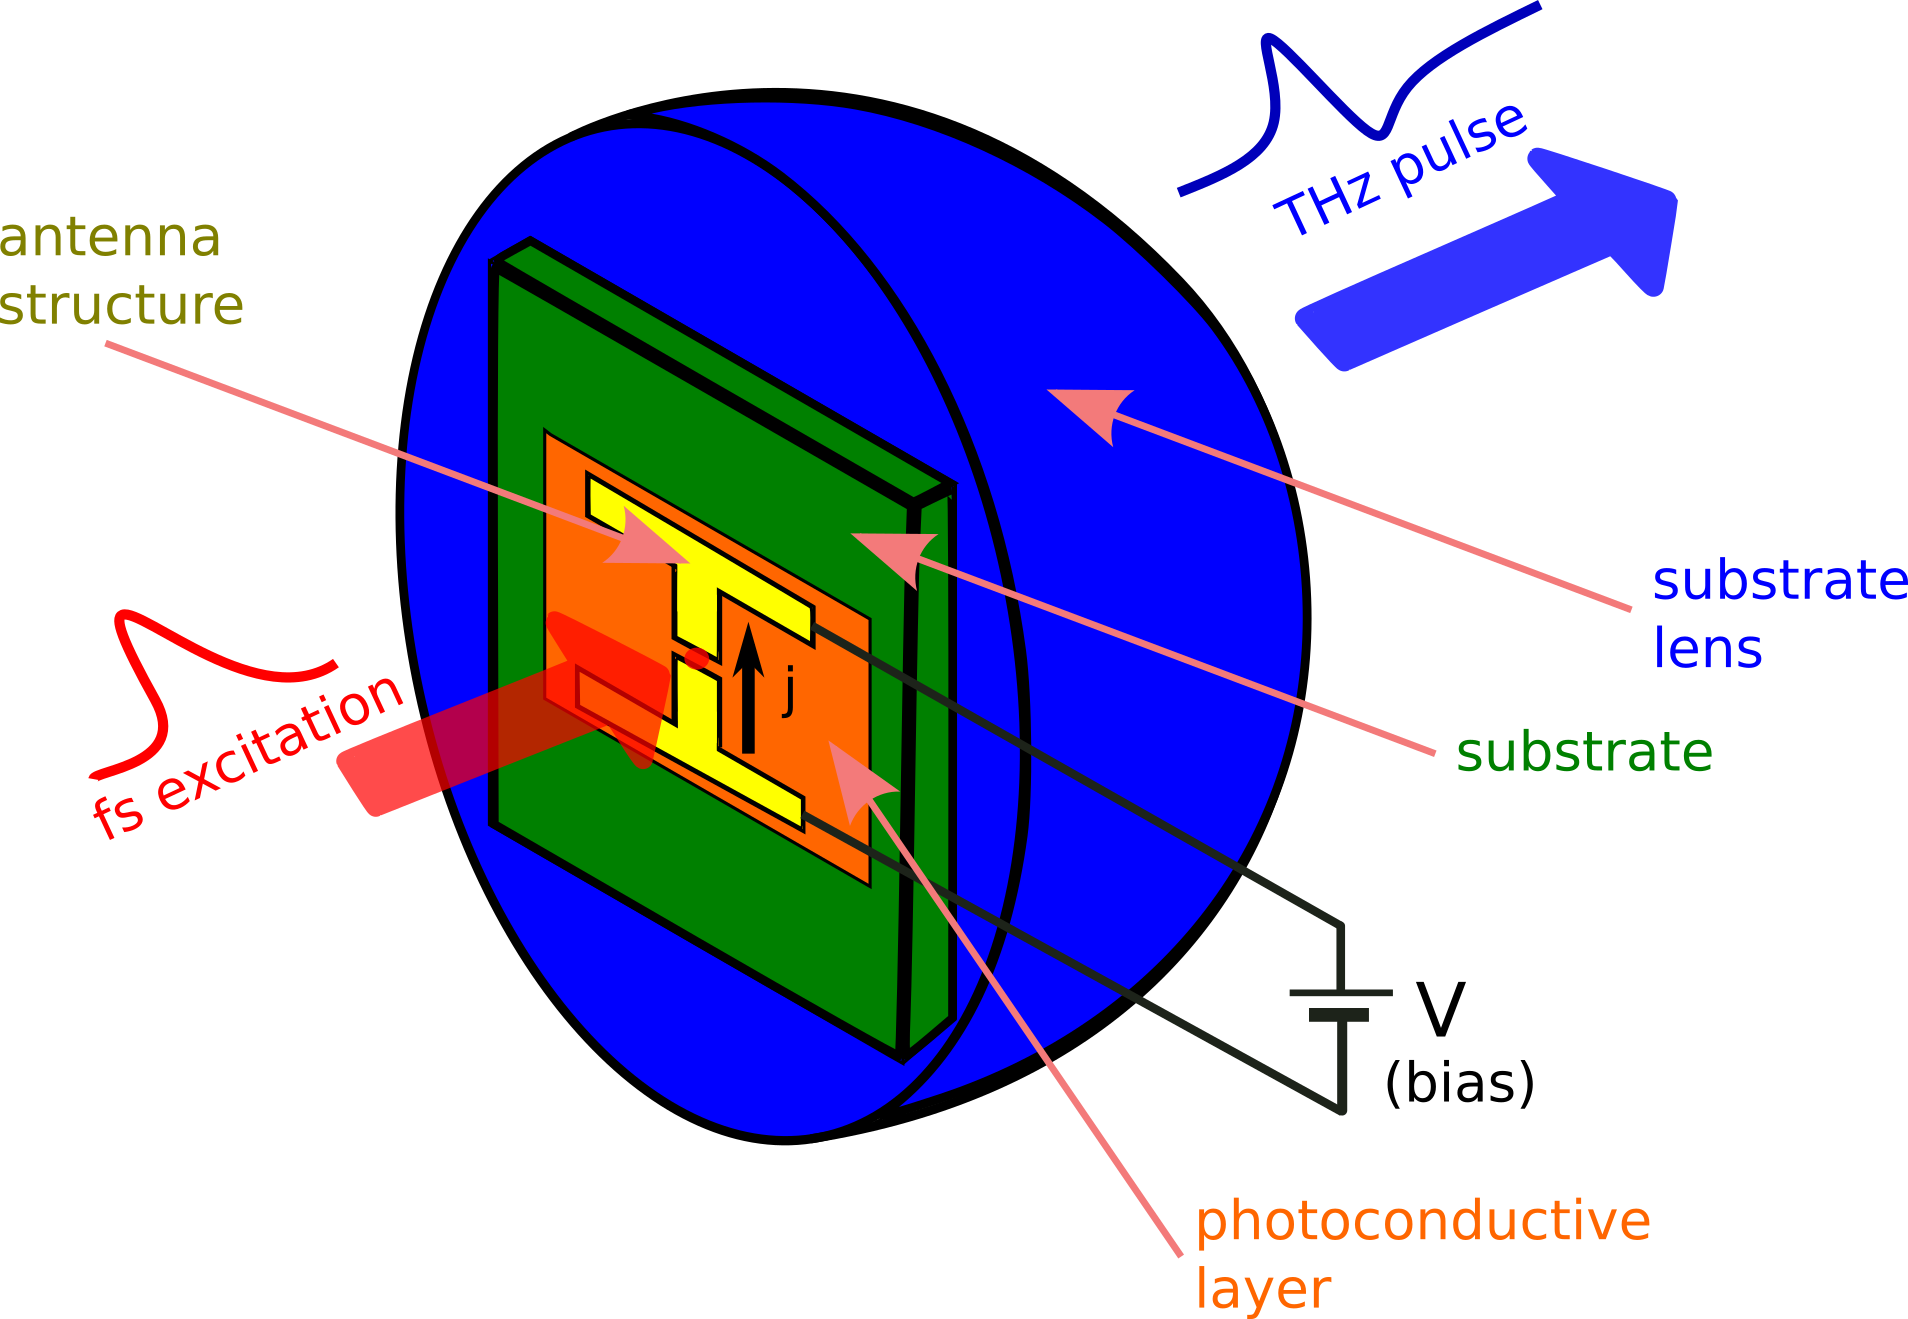
\includegraphics[scale=0.5]{images/TDS/PCA.png}
    \caption{Example of a PCA used for THz generation. The incoming laser pulse generates free charge carriers in the semiconductor substrate. The free charge carriers move due to the applied voltage so that a current flows between the anode and cathode. This high acceleration of the charge carriers causes them to emit radiation in the THz range. The shape of the silicon lens(shown in blue) prevents total internal reflection due to the high impedance difference.}
    \label{fig:PCA}
\end{figure}

The Drude-Lorentz model allows us to model the motion of the charge carriers which we assume to be predominantly consisting of electrons since they have a lower effective mass and therefore also a lower inertia compared to the holes. With this the photocurrent $j(t) = -e n(t) v(t)$ can be described via a coupled set of rate equations as follows:
\begin{equation}
    \frac{dn}{dt} = - \frac{n}{\tau_c} + G(t)
\end{equation}
\begin{equation}
    \label{eq:photocurrent_2}
    \frac{dv}{dt} = - \frac{v}{\tau_s} + \frac{e}{m^*}\left(E_0 - \frac{P_{sc}(t)}{\eta \epsilon} \right)
\end{equation}
\begin{equation}
    \frac{dP_{sc}(t)}{dt} = -\frac{P_{sc}(t)}{\tau_r}+j(t)
\end{equation}
where $n(t)$, $v(t)$, $e$ and $m^*$ denotes the density, velocity, charge and effective mass of the electrons respectively. $G(t)$ describes the increase of electron density in the illuminated area which therefore scales with the intensity of the laser pulse $I_L$. Additionally, due to the concurrent generation of holes and subsequent separation from the electrons an electric polarization $P_{sc}(t)$ is formed. This polarization field screens the local bias field $E_0$ where the screening strength is corrected by the effective permittivity $\epsilon$ of the semicondutor and the factor $\eta$, hence the correctional term to the field strength $E_0$ in equation \ref{eq:photocurrent_2}. The three times $\tau_c$, $\tau_s$ and $\tau_r$ serve as dampening factors and model different rate-lowering phyiscal processes which therefore depend on the semiconductor in question. This means that if we assume the shape of $G(t)$ then we can determine the generated current density \cite{Rutz2007}.

Furthermore, it is possible to show that the emitted electrical field is proportional to 
the change of the generated current density with time. To that extent we assume a dipole emission pattern; for a small gap size $d$ relative to the wavelength $(d \ll \lambda)$ and applying the far field approximation $(\lambda \ll r)$ the generated electric field can be described in spherical coordinates as follows:
\begin{equation}
    \label{eq:dipole_field}
    \bm{E_{THz}}(r, \theta, \omega) = -\frac{\mu_0 \sin \theta}{4\pi r} \omega^2 p(\omega) e^{i\omega r/c} \hat{\bm{\theta}},
\end{equation}
where $p(\omega)$ is the electric dipole moment, $\omega$ is the frequency and the z-axis is aligned parallel to the dipole moment \cite{Jackson1998}. We transform equation \ref{eq:dipole_field} into the time domain:
\begin{equation}
    \label{eq:dipole_field}
    \bm{E_{THz}}(r, \theta, t) = \frac{\mu_0 \sin \theta}{4\pi r} \partial_t^2 \mathcal{F}[p(\omega) e^{i\omega r/c}](t) \hat{\bm{\theta}} =
    \frac{\mu_0 \sin \theta}{4\pi r} \partial_t^2 p(t_r) \hat{\bm{\theta}},
\end{equation}
with the retarded time $t_r = t - r/c$ which ensures causality. In the context of this work it is worth noting that since the field only has one component it is expected that the emitted THz radiation is linearly polarized in the $\hat{\bm{\theta}}$ direction. Furthermore, using the continuity equation it is possible to show the following relation between the current density and the first time derivative of the dipole moment \cite{Griffiths2017}:
\begin{equation}
    \partial_t \bm{p}(t) = \int_{\mathbb{R}^3} \bm{j}(\bm{r}, t) d^3r = I_E.
\end{equation}
With this the previous relations can be summarized and linked as follows:
\begin{equation}
    E_{THz}(t) \propto \partial_t I_E(t) \propto \partial_t n(t) \propto \partial_t I_L(t),
\end{equation}
which means that the proportionality between the time derivative of the incident
laser pulse and the emitted THz radiation can be established. This can in theory be used for modeling of the emitted THz electric field based on the properties of the semiconductor and the incoming excitation pulse.

% To that extent: (Dachte es heisst so was wie "zu diesem Zweck")
% https://forum.wordreference.com/threads/in-so-far-to-that-degree-to-that-extent-so-far.1031704/
% https://forum.wordreference.com/threads/usage-of-to-that-extent-and-to-that-extend.1559032/
\section{Detection}
\label{sec:thz-detection}
PCAs can also be applied for the phase and amplitude resolved detection of THz waves. When employing a PCA as a detector, the THz radiation is coupled into the antenna substrate using a silicon lens and again on the other side a laser pulse is illuminating the photoconductive gap which generates free charge carriers in the substrate. In contrast to the emitter PCAs a bias is not applied. Instead the incoming THz pulse accelerates the charge carriers which results in formation of electric current. Therefore, by measuring this current signal at the electrodes as a function of time the THz pulse can be resolved. Unfortunately, it is not possible to resolve the current generated from a single THz pulse with resolution lower than a picosecond which is required. Therefore, utilizing the fact that identical THz pulses are generated periodically due to the constant repetition rate of the pulsed laser, multiple THz pulses can be sampled at different delays $\tau$ to scan the through the waveform. The delay can be varied by changing the optical path length of the laser pulse impinging on the detector. This can be accomplished with a mechanical delay line which moves a retroreflector and thereby varies the path length of the laser pulse to the detector. An example of a general THz-TDS setup in transmission geometry employing PCAs for detection and emission is shown in figure \ref{fig:Setup-THz-TDS-SimpleExample}. A retroreflector reflects the light in the direction of the incoming light but with a parallel shift. Assuming the retroreflector is moved a distance $s$ then the delay is twice the distance divided by the speed of light $c$: $\tau(s) = 2s/c$ \cite{Rutz2007}.  

\begin{figure}[H]
    \centering
    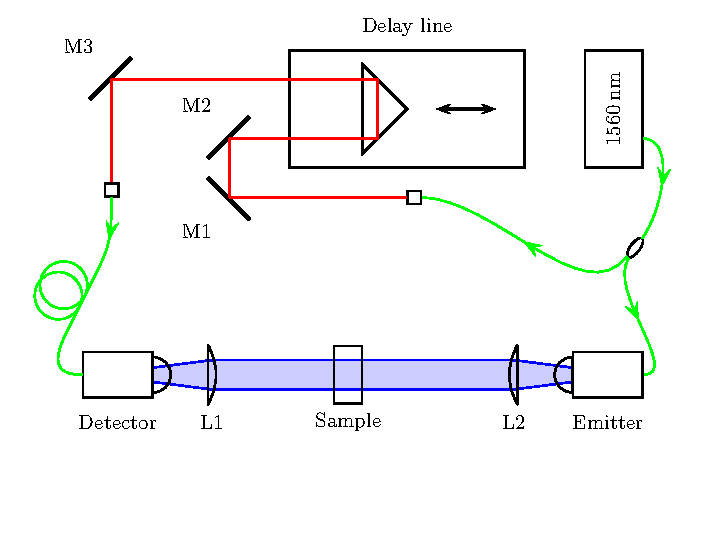
\includegraphics[scale=0.65]{images/TDS/Setup-THz-TDS-SimpleExample.pdf}
    \caption{Example of a general THz-TDS setup in transmission geometry employing PCAs as detector and emitter. The laser pulses are guided using mirrors M1-M3. Two polyethylene lenses (L1, L2) are used to collimate the THz radiation and focus it on the detector module.}
    \label{fig:Setup-THz-TDS-SimpleExample}
\end{figure}

Additional examples of THz-TDS spectrometers are presented in chapter \ref{ch:setups} which utilize the emission and detection scheme described in this chapter. These two setups were used for a part of the measurements performed in this work. In the following chapter we introduce the fundamentals of EM wave polarization including different mathematical (and graphical) representations of the polarization state as well as the propagation of light in anisotropic media.

\chapter{Polarization of light}
\label{ch:theory}
%In this chapter we will introduce the basic underlying physical principles of birefringent waveplates. Simply put, the purpose of a waveplate is to modify the polarization state of EM waves in a controlled way as they pass through the waveplate. This is most commonly achieved by fabricating plates with a certain thickness from a birefringent material. To this end, we first describe the polarization ellipse in section \ref{sec:polellipse}. Following this the underlying physical principles birefringence and dichroism are explained in more detail in section \ref{sec:wave_prop}. Finally, in section \ref{sec:waveplates} we then show what role these two principles play in regards to waveplates. Any change to a polarization state and the polarization states themselves, can be described mathematically using the Jones calculus which will be shown in section \ref{sec:math_desc}. At the end this leads up to the description of achromatic composite waveplates and the design as it is used in this work. Both are presented in section \ref{sec:jonescalc} of this chapter.
In this chapter we introduce the underlying physical principles of birefringent waveplates. Simply put, the purpose of a waveplate is to modify the polarization state of EM waves in a controlled way as they pass through the waveplate. This is most commonly achieved by fabricating plates with a certain thickness from a birefringent material. We therefore first describe the polarization ellipse in section \ref{sec:polellipse} which is an intuitive representation of the polarization state of an EM wave. Following this, in section \ref{sec:wave_prop} the physical principles birefringence, form birefringence and dichroism are explained. At the end of the section we discuss the Fresnel coefficients in the special case of non-aligning anisotropic media. In the final section \ref{sec:math_desc} of this chapter we introduce three additional representations of the polarization state which compared to each other have certain advantages and disadvantages.

\section{The polarization ellipse}
\label{sec:polellipse}
Simply put, the polarization or polarization state of an EM wave is the direction in which the wave is oscillating. There are several ways to describe or represent the polarization state of EM waves. One of them is the polarization ellipse which is a geometrical representation of the polarization state. This remained the only satisfactory way to visualize the different polarization states for almost the entire 19\textsuperscript{th} century, although it is not very practical for carrying out calculations. At the end of the century another representation was proposed by Henri Poincaré, now known as the Poincaré sphere, which could be used for both calculations and visualization of the polarization states \cite{Collett2008a}. 

Poincaré's representation will be explained in section \ref{sec:math_desc}. The polarization ellipse can be derived either directly from a solution to the EM wave equation or starting from Maxwell's equations. It is practical to start from Maxwell's equations, since they are used for derivations later on in this work. In differential form Maxwell's equations are given by:
\par
\noindent\begin{minipage}{.5\linewidth}
\begin{align}
    \bm{\nabla}\cdot\bm{D} &=\rho_{f}\;,\label{eq:maxwell1}
    \vphantom{\frac{\partial\bm{B}}{\partial t}}\\
    \bm{\nabla}\cdot\bm{B} &=0\;,\vphantom{\frac{\partial\bm{B}}{\partial t}}\label{eq:maxwell2}
\end{align}
\end{minipage}%
\begin{minipage}{.5\linewidth}
\begin{align}
    \bm{\nabla}\times\bm{E} &=-\frac{\partial\bm{B}}{\partial t}\;,\label{eq:maxwell3}
    \\
    \bm{\nabla}\times\bm{H} &=\bm{J}_f
    +\frac{\partial\bm{D}}{\partial t}\;,\label{eq:maxwell4}
\end{align}
\end{minipage}
\newline

where $\bm{E}, \bm{H}$ denote the electric and magnetizing fields respectively,  $\bm{D}=\hat{\epsilon} \bm{E}$ is the electric displacement for a linear medium, $t$ is the time and $\hat{\epsilon}$ is the permittivity which depends on the material and is a complex function of the frequency. The materials used in this work are non magnetic, which means that the magnetic and magnetizing fields are proportional: $\bm{B} = \mu_0 \bm{H}$, where $\mu_0$ denotes the vacuum permeability. $\rho_f, \bm{J}_f$ are the free charge and current density, respectively. Usually in optics there are no free charge carriers or free currents, which is also the case for all materials in this work, so we set $\rho_f=\bm{J}_f=0$ \cite{Roth2019}. If we then further assume that the materials are homogeneous so that $\hat{\epsilon}$ does not depend on position, then we can reduce equations \ref{eq:maxwell1}-\ref{eq:maxwell4} to the following symmetrical set of equations:

\noindent\begin{minipage}{.5\linewidth}
\begin{align}
    \bm{\nabla}\cdot \bm{E} &=0\;,\label{eq:maxwell1reduced}
    \vphantom{\frac{\partial\bm{B}}{\partial t}}\\
    \bm{\nabla}\cdot\bm{B} &=0\;,\vphantom{\frac{\partial\bm{B}}{\partial t}}\label{eq:maxwell2reduced}
\end{align}
\end{minipage}%
\begin{minipage}{.5\linewidth}
\begin{align}
    \bm{\nabla}\times\bm{E} &=-\frac{\partial\bm{B}}{\partial t}\;,\label{eq:maxwell3reduced}
    \\
    \bm{\nabla}\times\bm{B} &=\mu_0 \hat{\epsilon} \frac{\partial\bm{E}}{\partial t}\;,\label{eq:maxwell4reduced}
\end{align}
\end{minipage}
\newline

Applying the curl to equation \ref{eq:maxwell3reduced} and with equation \ref{eq:maxwell4reduced} we can decouple $\bm{E}$ and $\bm{B}$: 
\begin{equation}
    \bm{\nabla}\times \bm{\nabla}\times \bm{E} = -\mu_0 \hat{\epsilon} \frac{\partial^2\bm{E}}{\partial t^2}
\end{equation}
Then using the vector calculus identity: $\bm{\nabla}\times \bm{\nabla}\times \bm{F} = \bm{\nabla} \left( \bm{\nabla} \cdot \bm{F} \right) - \bm{\nabla}^2 \bm{F}$, for any vector field $\bm{F}$, together with equation \ref{eq:maxwell1reduced} we get the EM wave equation: \footnote{We neglect the magnetic field, since we are only concerned with non magnetic materials in this work. Nevertheless, the derivation of the wave equation for the magnetic field looks similar to the derivation for the electric field.}
\begin{equation}
    \label{eq:waveeq}
    \bm{\nabla}^2 \bm{E} = \mu_0 \hat{\epsilon} \frac{\partial^2\bm{E}}{\partial t^2}
\end{equation}
and via a Fourier transform $(\mathcal{F}[\partial_t f(t)](\omega) \xrightarrow{} i\omega \mathcal{F}[f(t)](\omega))$ we readily obtain the wave equation in frequency space also known as the Helmholtz equation for $\bm{E}$:
\begin{equation}
    \label{eq:waveeqfreq}
    \bm{\nabla}^2 \bm{E} = -\mu_0 \hat{\epsilon} \omega^2 \bm{E},
\end{equation}
where $\omega$ is the angular frequency.
A solution to the wave equation is a monochromatic coherent plane wave with a frequency $\nu=\frac{\omega}{2\pi}$ which can be written as: 
\begin{equation}
    \label{eq:planewave}
    \bm{E} = \bm{E_0} e^{i(\bm{k}\bm{r} - \omega t + \delta)},
\end{equation}
where $\bm{r}$ and $\bm{k}$ denote the position and wave vector respectively, $\bm{E_0}$ is a complex vector which denotes the maximum amplitude and oscillation direction of the wave, $\delta$ is the phase constant. If we assume the wave propagates along the z-direction in a Cartesian coordinate system, then the amplitude will be orthogonal to the z-direction, i.e a transverse wave. This follows directly from equation \ref{eq:maxwell1reduced}. From the Helmholtz equation we then find the requirement that the wave number, which is the magnitude of the wave vector, and the angular frequency are related by:
\begin{equation}
    \label{eq:wavevector_req}
    k = \sqrt{\mu_0 \hat{\epsilon}} \omega
\end{equation}
The phase velocity $v$ of the wave can then be expressed as:
\begin{equation}
    v = \frac{\omega}{k} = \frac{1}{\sqrt{\mu_0 \hat{\epsilon}}} = \frac{c}{n},\:n = \sqrt{\frac{\hat{\epsilon}}{\epsilon_0}},
\end{equation}
where $c$, $\epsilon_0$ and $n$ are the speed of light in vacuum, vacuum permittivity and refractive index, respectively. This way we get from the wave equation two decoupled equations, each describing an oscillation in the xz-plane and the yz-plane. This is also known as Fresnel's wave theory which was proposed and verified experimentally around 1820 by Augustin-Jean Fresnel and François Arago, more than 40 years before Maxwell's equations were published \cite{Collett2009,Jackson1998}.

This means that equation \ref{eq:planewave} consists of only two perpendicular components. Additionally, if we consider that Maxwell's equations \ref{eq:maxwell1reduced}-\ref{eq:maxwell4reduced} are all linear and real, then it follows that the real part of any particular solution is also a solution to the wave equation. \footnote{It is worth noting that this only works if the equations are real. For example, Schrödinger's equation is linear but complex, therefore even if $\psi$ is a solution $\operatorname{Re}(\psi)$ and $\operatorname{Im}(\psi)$ are not.} We can then write equation \ref{eq:planewave} as two sinusoidal waves:
\begin{equation}
\label{eq:plane_wave_realparts}
\begin{aligned}
    E_x(z, t) = E_{0x}\cos(kz-\omega t + \delta_x) \\
    E_y(z, t) = E_{0y}\cos(kz-\omega t + \delta_y), 
\end{aligned}
\end{equation}
where $\delta_x$ and $\delta_y$ are arbitrary phases of the two components. Depending on the values of $E_{0x}, E_{0y}$ and the relative phase or simply phase, which is $\delta = \delta_y - \delta_x$, we describe different polarization states. Figure \ref{fig:Ex_Ey_planewaves} shows the real parts of the two plane wave components for a wave traveling along the z-direction when $\delta=0$ and $E_{0x}=E_{0y}$.

\begin{figure}[h]
    \centering
    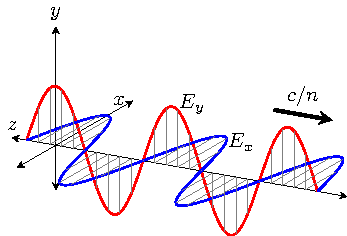
\includegraphics[scale=1]{images/theory/tikz_e_wave.pdf}
    \caption{Two sinusoidal waves given by equation \ref{eq:plane_wave_realparts}, which are the real parts of the plane wave components. Both waves have the same amplitude and phase.}
    \label{fig:Ex_Ey_planewaves}
\end{figure}

With this in place we can visualize the different polarization states, that is the different directions the electric field, or simply the light, can oscillate in. If the light is confined to a plane along the direction of propagation it is said to be linearly polarized (LP), this plane is known as the polarization plane. An example of this is shown in figure \ref{fig:E_planewave}, where the polarization plane is at an angle of \SI{45}{\degree} relative to the x-axis. 

\begin{figure}[h]
    \centering
    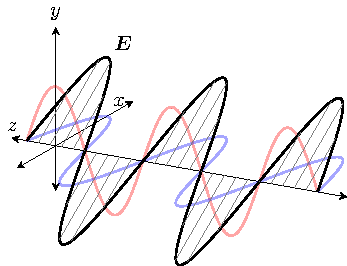
\includegraphics[scale=1.1]{images/theory/tikz_linear_pol.pdf}
    \caption{The black curve shows the superposition of the two sinusoidal waves from equation \ref{eq:plane_wave_realparts}, which is the same as the real part of a LP plane wave at an angle of \SI{45}{\degree} to the x-axis. In addition, the horizontal and the vertical components of the field vector are shown as the red and blue curves respectively.}
    \label{fig:E_planewave}
\end{figure}

Now, if $\delta$ is exactly $\nicefrac{\pi}{2}$ and $E_{0x} = E_{0y}$, then we have the case shown in figure \ref{fig:circ_pol_planewave} (b). A field with this kind of polarization traces out a circle as time passes for a fixed position in space. On the other hand, if we keep time fixed then the field vector describes a helix along the direction of propagation. This means that the field only changes direction but not its magnitude. This type of polarization is therefore called circular polarization (CP). Additionally, because we can trace out a circle in two different directions (clockwise or counterclockwise) we can therefore distinguish between two different types of circular polarizations. These two types are called left CP (LCP) or right CP (RCP) depending on the direction the circle is traced out, either in a left- or right-handed sense. This is called the handedness of the light, which can be determined using the right hand rule. For that we fix the right hand at a point on the helix and point the thumb away from the receiver, that is against the direction of propagation. Then the light is right-handed if the helix is traced out in the direction of the other fingers as time evolves, otherwise it is left-handed. The light shown to the left of figure \ref{fig:circ_pol_planewave} is therefore left-handed while the example on the right side of figure \ref{fig:circ_pol_planewave} shows right-handed CP light. The reason why we have two types of CP in the first place, is the fact that one component can lead the other, as we can see in figure \ref{fig:circ_pol_planewave}. Where for RCP the horizontal component leads the vertical one by a quarter period $\left(\delta = \frac{\pi}{2}\right)$, for LCP it is the other way around and $\delta = -\frac{\pi}{2}$. 


\begin{figure}
\centering
\subcaptionbox{\label{fig:circ_pol_planewave_a}}
    {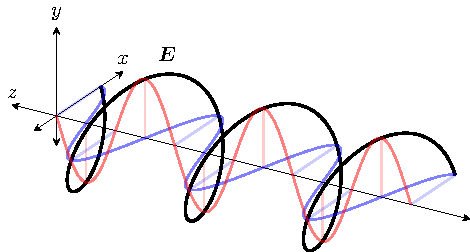
\includegraphics[scale=0.8]{images/theory/tikz_circ_pol_lh.pdf}}
\subcaptionbox{\label{fig:circ_pol_planewave_b}}
    {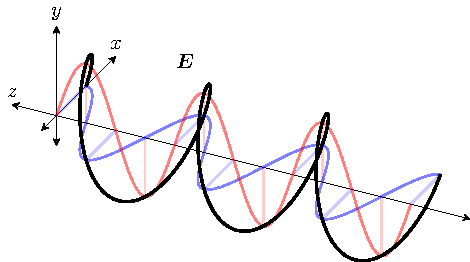
\includegraphics[scale=0.8]{images/theory/tikz_circ_pol_rh.pdf}}
\caption{The left figure shows an example of LCP light and the right figure RCP light. Furthermore, handedness originates from one component leading the other. In the case of LCP light the vertical component leads the horizontal component and vice versa for RCP light.}
\label{fig:circ_pol_planewave}
\end{figure}

Finally, the last polarization state we have not mentioned yet, even though it is in fact the most general, is the elliptical polarization state. The polarization states we have dealt with so far have all been limiting cases of this state. For a fixed position this is fairly simple to visualize geometrically; LP light traces out a line while CP light traces out a circle, both of these shapes are degenerate forms of an ellipse. A summary of the different degenerate states and the corresponding amplitude and phase combinations are shown in table \ref{tab:pol_state_summary}, which is divided into three parts with a pair of states in each. The linear horizontal/vertical polarization (LHP/LVP) states are at the top, the linear $\pm\SI{45}{\degree}$ polarization ($L_{\pm45}P$) states are in the middle and the CP states are at the bottom. The last column shows the corresponding degenerate ellipse for each state.

\begin{table}[h]
    \centering
    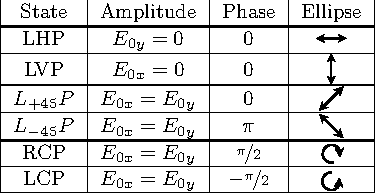
\includegraphics[scale=1]{images/theory/pol_summary_table.pdf}
    \caption{Summary of the different degenerate polarization states, with corresponding representing symbols. The first four states are linearly polarized at different angles relative to the x-axis; $\SI{0}{\degree}$, $\SI{90}{\degree}$, $\SI{45}{\degree}$ and $\SI{-45}{\degree}$ respectively. The last two are the RCP and LCP states.}
    \label{tab:pol_state_summary}
\end{table}

We can also realize this mathematically by eliminating the time and position dependency of the two components in equation \ref{eq:plane_wave_realparts}, so that we get \footnote{The derivation is given in \ref{sec:deriv_pol_ellipse}}:

\begin{equation}
    \centering
    \label{eq:pol_ellipse}
    \frac{1}{\sin^2 \delta} \left[ \left(\frac{E_x}{E_{0x}}\right)^2+\left(\frac{E_y}{E_{0y}}\right)^2-2\frac{E_x E_y}{E_{0x} E_{0y}}\cos \delta \right]=1,
\end{equation}

which describes an ellipse in its nonstandard form. Because of this the equation is called the polarization ellipse. It is worth noting that even though the time and position dependencies have been explicitly eliminated, the wave components $E_x$ and $E_y$ continue to depend on them. That means $E_{0x}$, $E_{0y}$ and $\delta$ are the polarization ellipse parameters, which define the shape of the ellipse. Therefore, the shape of the ellipse is independent of time and position. There are several ways to parameterize the polarization ellipse or ellipses in general using two parameters. One way is to use the orientation angle $\psi$ and the ellipticity angle $\chi$, which both can be expressed through the polarization ellipse parameters: 

\begin{equation}
    \label{eq:ellipse_orientation}
    \tan 2\psi = \frac{2E_{0x}E_{0y}}{E_{0x}^2 - E_{0y}^2}\cos \delta = 
    \tan 2\alpha \cos \delta
    ,\: 0\leqslant\psi\leqslant\pi,
\end{equation}
\begin{equation}
    \label{eq:ellipse_ellipticity}
    \sin 2\chi = \frac{2E_{0x}E_{0y}}{E_{0x}^2 + E_{0y}^2}\sin \delta = 
    \sin 2\alpha \sin \delta,\: \nicefrac{-\pi}{4}\leqslant\chi\leqslant\nicefrac{\pi}{4},
\end{equation}
where we have defined $\tan \alpha = \frac{E_{0y}}{E_{0x}}$ so that $\alpha$ and $\delta$ constitute another set of parameters associated with a second equivalent parameterization. Figure \ref{fig:pol_ellipse} shows an example of a polarization ellipse together with the orientation and ellipticity angles. We see from the figure that for $\psi = 0, \pi$ or $\psi = \frac{\pi}{2}$ the major and minor axes $(a$ and $b)$ coincide with the coordinate axes. Likewise for $\chi = 0$ the ellipse degenerates to a line and for $\chi = \pm\frac{\pi}{4}$ we get a circle \cite{Collett2009}. Actually, in most cases a light beam is a mixture of different polarization states, this is referred to as unpolarized light. It consists of a high number of short wave trains which are emitted from the individual atoms. In most cases these wave trains are radiated from dipoles and are therefore linearly polarized, but since every atom oscillates in a different direction the polarization will also vary for each wave train. Hence, the beam will be a mixture of different states \cite{Roth2019}. However, as we saw in the previous chapter we expect that the THz radiation emitted from PCAs is strongly linearly polarized.
% TODO $\psi = 0, \pi$ or $\psi = \frac{\pi}{2}$ ???
\begin{figure}[h]
    \centering
    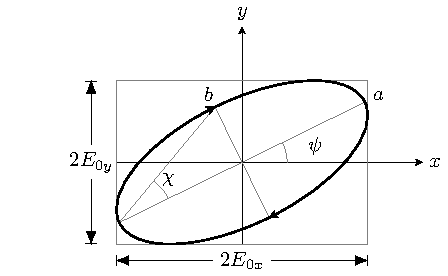
\includegraphics[scale=1.0]{images/theory/tikz_pol_ellipse.pdf}
    \caption{Example of a polarization ellipse, which shows the ellipticity $\chi$ and orientation angle $\psi$ geometrically. The major and minor axes of the polarization ellipse are denoted by $a$ and $b$ respectively. We see that $\chi$ changes with the shape of the ellipse while $\psi$ is simply the orientation relative to the x-axis.}
    \label{fig:pol_ellipse}
\end{figure}

We finish off this section, as a bit of a side note, by mentioning the conventions used so far. If we go back to the plane wave solution (equation \ref{eq:planewave}) of the wave equation we see that a replacement of $i$ with $-i$ yields another valid linearly independent solution. This leads to two different sets of definitions, depending on the sign of the imaginary unit. The first one, with a positive sign and the one used here, is commonly used in physics texts. While the other one with a negative sign is mainly used in electrical engineering (EE) texts. Mathematically, the difference between these two conventions is simply the direction of rotation of the phasor\footnote{Here phasor simply refers to the complex representation of $A\cos(\omega t + \delta)$} in the complex plane with increasing time. An example of this is shown for a phasor $x$ in figure \ref{fig:phasor}. 

\begin{figure}[h]
    \centering
    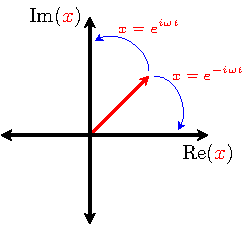
\includegraphics[scale=1.3]{images/theory/tikz_phasor_rotation.pdf}
    \caption{Example of a phasor $x$ in the complex plane. The sign of the imaginary unit determines the direction of rotation for increasing times. The rotation is indicated by the blue arrows and is either in the clockwise $(-i)$ or counterclockwise $(+i)$ direction.}
    \label{fig:phasor}
\end{figure}

The choice of sign does not affect only the direction of the phasor rotation but it also has other implications. We know from equation \ref{eq:wavevector_req} that the wavevector is in general complex because the permittivity is complex, so we can write it as $k=\tilde{\beta} + i \tilde{\alpha}$. On the other hand we obtain two expressions for a plane wave propagating in the z-direction, one for each definition:
\begin{align}
    &\bm{E_{0}}e^{i((\tilde{\beta} + i \tilde{\alpha})z-\omega t + \delta)} \\
    &\bm{E_{0}}e^{-i((\tilde{\beta} + i \tilde{\alpha})z-\omega t + \delta)}, 
\end{align}
if we factor out the $\tilde{\alpha}$ dependency we get:
\begin{align}
    e^{-\tilde{\alpha} z}&\bm{E_{0}}e^{i(\tilde{\beta} z-\omega t + \delta)} \\
    e^{\tilde{\alpha} z}&\bm{E_{0}}e^{-i(\tilde{\beta} z-\omega t + \delta)}. 
\end{align}
We see that in case of the EE definition the amplitude would increase as the wave propagates, which is nonsense. Therefore the sign of the imaginary part of the wavevector must be chosen accordingly. So for the EE definition we get:
\begin{equation}
    k=\tilde{\beta} - i \tilde{\alpha}
\end{equation}
and 
\begin{equation}
    k=\tilde{\beta} + i \tilde{\alpha}
\end{equation}
for the physics definition.
As a result the sign of the imaginary part of the refractive index will also depend on the chosen definition. When the EE definition is used:
\begin{equation}
    \tilde{n}= n - i \kappa
\end{equation}
and using the physics definition:  
\begin{equation}
    \tilde{n}= n + i \kappa.
\end{equation}

The physics definition is used for example in the textbooks by John D. Jackson \cite{Jackson1998} and David J. Griffiths \cite{Griffiths2017} and also in \cite{Collett2009}, which is the reference used for most of this section.
There are not only convention differences between engineers and physicists but also even between different branches of physics. The definition of CP handedness relies on the point of view; that is either looking from the source in the direction of propagation or from the receiver against the direction of propagation. Here we use the version which is defined from the point of view of the receiver. This is also the convention commonly used in optics \cite{Bass1995, M.LandiDeglInnocenti2004} as well as by SPIE \cite{Collett2009}.
The other convention is used by radio astronomers \cite{Born1999}, quantum physicists, because it is consistent with the convention of handedness for a particle's spin and it is also used by electrical engineers \cite{Orfanidis2004}.

\section{Light propagation in anisotropic media}
\label{sec:wave_prop}
In the previous section we saw that the electric field consists of two perpendicular components which trace out an ellipse with the advancement of time for any fixed position. Additionally, the shape and orientation of the ellipse depend on the relative phase of the two components as well as their amplitudes. Naturally this dependency is symmetrical in the two amplitudes and the relative phase, as can be seen directly from equations \ref{eq:ellipse_orientation} and \ref{eq:ellipse_ellipticity}. Therefore, to change the polarization state, the two phases or the two amplitudes must be changed by different amounts. Otherwise simply the scale of the ellipse changes and not its shape or orientation. Consequently, for this to happen the medium the wave is propagating in must be anisotropic. Now, if the absorption of the material is direction dependent, then the amplitude will vary differently for the two components. Materials with this property are said to be dichroic. Likewise, some materials cause different phase changes between the two components. This material property is called birefringence. In the following section we will explain these two properties phenomenologically as well as their underlying physical principle.

\subsection{Dichroism}
\label{sec:dichroism}
In general, the term dichroism refers to the selective absorption of one of the two perpendicular field components of the light. Materials with this property are said to be dichroic. This can be used for example in polarizers, which are extremely anisotropic so that one component is ideally completely extinguished by the polarizer, while it is transparent for the other field component. The simplest polarizer of this sort is a grid of parallel conducting wires as it is shown in figure \ref{fig:wire_grid_polarizer} which is also known as a wire grid polarizer (WGP). The WGP is similar to a conducting diffraction grating with a sub-wavelength period. Now, if we assume that the light initially is unpolarized as it propagates towards the wire grid from the left, then the light will be linearly polarized perpendicular to the wires after the WGP. We can see this by considering the interaction of the two field components with the wires separately. One component can then be set to be parallel to the wires and the other perpendicular. The electrons are free to move in the y-direction, because the wires are conducting, so that a current is generated due to the acceleration of the electrons by the parallel field component. This current results in joule heating of the wires so that a part of the energy of the electric field is turned into heat. Additionally, the accelerated electrons radiate in both the forward and backward directions. The part that is radiated forwards, along the direction of propagation, mostly cancels the transmitted incident wave and the other part appears as the reflected wave. On the other hand, the electrons along the x-direction, that is perpendicular to the wires, are not free to move very far so that the corresponding wave component passes almost freely. So, at the end the component parallel to the wires is mostly extinguished and the light is therefore linearly polarized perpendicular to the wires \cite{Hecht}.

\begin{figure}[h]
    \centering
    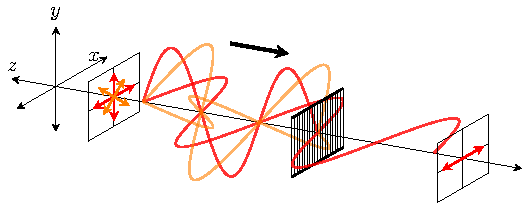
\includegraphics[scale=1.30]{images/theory/tikz_wire_grid_polarizer.pdf}
    \caption{A schematic of a wire grid polarizer which is essentially a conducting sub-wavelength grating. From the left unpolarized light interacts with the wire grid so that the field components parallel to the wires are eliminated. After passing the polarizer the light is therefore linearly polarized perpendicular to the wires.}
    \label{fig:wire_grid_polarizer}
\end{figure}

It has been shown that it is possible to polarize even visible light using these wire grids. In 1960 George R. Bird and Maxfield Parrish fabricated a WGP having 2160 wires per mm, making it suitable for Near-Infrared light \cite{Bird1960}. Naturally, WGPs also exist for the lower THz-range. An example of this is an aluminum-based WGP with a frequency range of \SIrange{0.3}{2.5}{\tera \hertz} and an extinction ratio ranging from \SI{45}{\dB} for lower frequencies and \SI{30}{\dB} for the higher ones. The extinction ratio is simply the ratio of the transmitted power coefficients for the field components perpendicular and parallel to the wires in decibel, so it is a measure of how well the light is only transmitted perpendicular to the wires after passing the polarizer \cite{Ferraro2016}. 
In contrast to a WGP some materials are inherently dichroic. For example the mineral tourmaline has a particular axis, which in general is called the optic axis, light propagating parallel to this axis experiences a smaller absorption coefficient compared to any other direction. Additionally, this selective absorption depends on the wavelength of the light. Therefore if the crystal is illuminated with white polarized light, then the absorbed colors will change depending on the polarization and so the crystal will change color depending on the polarization. This is where the name dichroic comes from, meaning two colors. The mechanism that gives rise to dichroism in crystals can be explained by considering its microscopic structure. The electrons bound to the lattice points of the crystal interact with electrons bound to other nuclei, especially the nearest neighbors. So if the crystal lattice is asymmetrical then the binding forces of the electrons will also be asymmetrical resulting in a polarization dependent response. Additionally, if the conductivity depends on the direction so will the amount of joule heating generated due to the induced currents. As a consequence the absorption will be direction dependent. 

To summarize, in this section we discussed two types of dichroism; one originating from a non-zero anisotropic conductivity of the structure on a macroscopic scale explained using the example of a WGP and the other type arising from asymmetries on the atomic scale. Loosely speaking, the effects of dichroism and birefringence in the cases relevant for this work can be explained by a direction and polarization dependent imaginary and real part of the refractive index, respectively. This complicates the description of EM wave propagation in anisotropic materials, as we will see in the following section which introduces the most relevant concepts related to birefringence \cite{Hecht}.

\subsection{Birefringence}
\label{sec:birefringence}
Birefringence is the material property responsible for the phenomenon of double refraction. This phenomenon was observed for the first time in calcite crystals by the Danish scientist Rasmus Bartholin in 1669 \cite{RasmusBartholin1669, Restaino2015}. The effect of double refraction on a light beam passing through a birefringent material is relatively easy to show. One can simply place a birefringent crystal on top of some text, as it is shown in figure \ref{fig:3birefringence}. Two images of the text become visible through the crystal and each image is shifted by a different amount. These images are not simply reflections at the crystal-air interface, since the images are brighter compared to images formed through reflections, and they are even visible when looking down directly from above. Also if the crystal is rotated then one of the images will be stationary, while the other one will circle around the stationary image. The waves forming the stationary image are known as the ordinary waves (o-rays or o-waves), while the ones forming the moving image are called extraordinary waves (e-rays or e-waves) as suggested by Bartholin at the discovery of the phenomena. The same effect can be illustrated by sending a beam of unpolarized light through the crystal. The beam is split in two as it propagates through the crystal. One can show, using a WGP or any other polarizer, that the polarization states of the two beams are orthogonal \cite{Roth2019}.

\begin{figure}[h]
    \centering
    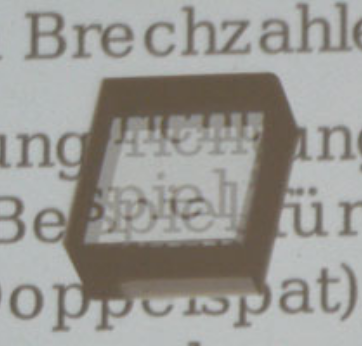
\includegraphics[scale=0.25]{images/theory/birefringence.png}
    \caption{A calcite crystal placed on top of some text. This demonstrates the effect of birefringence on the original image seen through the crystal. Source: \cite{Roth2019}.}
    \label{fig:3birefringence}
\end{figure}

The explanation of the underlying physical principle of birefringence is similar to that of dichroism; it can be explained by considering the structure of the material. We can represent the binding of the electron cloud to the nucleus at each crystal lattice point using a harmonic oscillator model. The model, which is shown in figure \ref{fig:electron_shell}, consists of a shell bound to the nucleus with springs. Furthermore, the springs have different spring constants and the nucleus is fixed in space. So, if an electron is displaced parallel to one of the springs it will oscillate with a different frequency relative to any other direction. How this finally influences the refractive index can be explained by considering the propagation of light through a transparent medium. As the wave propagates through the medium the electric field excites the electrons which then in turn reradiate because any accelerating charge emits radiation. These reradiated wavelets recombine to form the refracted wave. Additionally, the phase velocity of the refracted wave will be determined by the frequency difference between the natural oscillation of the electrons and the frequency of the electric field. Since the refractive index is simply the ratio between the speed of light in vacuum and in the medium it will change depending on this frequency difference as well. If we go back to figure \ref{fig:electron_shell} this means that for example a wave linearly polarized parallel to the x-axis experiences a different refractive index compared to the one polarized parallel to the z-axis. That is also the definition of birefringence; a material with two or more different refractive indices. 

\begin{figure}[h]
    \centering
    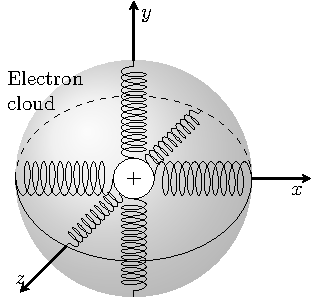
\includegraphics[scale=0.9]{images/theory/tikz_electron_shell.pdf}
    \caption{Lorentz oscillator model of an electron cloud, which is represented by a negatively charged spherical shell. It is bound to its positively charged nucleus via springs of different strength. The mass of the nucleus is assumed to be infinite so that it is fixed in space. This model is a simplification of an optical anisotropic material, for an isotropic material the spring constants would all be equal.}
    \label{fig:electron_shell}
\end{figure}

At this point it is worth making a few general remarks about this mechanical spring model before we continue with the concepts related to birefringence. The model is called the Lorentz oscillator model after Hendrik Antoon Lorentz who first devised this theory in the late nineteenth century. This was before the discovery of quantum mechanics and it was therefore originally purely a classical model. The model was then later adapted to quantum mechanics and is still often used to describe the interaction between atoms and electric fields. Lorentz did not assume that the electron was actually bound to the nucleus by a physical spring but rather that the force could be approximated by a harmonic oscillator. This is a justified assumption since any kind of binding force can be approximated by a harmonic oscillator, if the displacement is small enough so that only the linear terms in the Taylor expansion are significant. However, this classical version of the model fails to explain a large number of the observed effects, especially when a weak field is interacting with a small number of atoms. For this situation and others, at least a partially quantum mechanical description is required. As an example, in \cite{Rerat2020} the birefringence is calculated using a quantum mechanical treatment \cite{doi:https://doi.org/10.1002/9780470409718.ch3}. Nonetheless, the Lorentz oscillator model is sufficient for the description of the phenomena in the context of this work. For the rest of this section we will therefore explain the phenomena introduced at the start of the section based on the Lorentz model and then present a few more useful concepts to finish off the section. A concept that is helpful in understanding the phenomena is the optic axis of a crystal\footnote{In the context of crystals it is called the optic axis, otherwise it is called the optical axis like the axis perpendicular to the center of a lens \cite{Hecht}.}. That is, if we have the case in which two springs have the same rigidity, for example those in the xy-plane, then the optic axis will be parallel to the z-axis. The special property of the optic axis is that any wave propagating parallel to it will only experience one refractive index, because the material is optically symmetrical under any rotation about this axis. This means that the two components of the wave, which are perpendicular to the direction of propagation, will experience an isotropic medium and therefore the same refractive index. Since this symmetry exists at every lattice point, the optic axis is actually a direction and not just a line through a single point \cite{Hecht}. 

Furthermore, this explains the phenomena described at the beginning of this section. Going back to the calcite crystal shown in figure \ref{fig:3birefringence} we see that the optic axis must be at an angle, not parallel or perpendicular, to the surface normal. Otherwise we would not observe double refraction. Additionally, considering that the light is unpolarized, the field components perpendicular to the optic axis will not be refracted and they therefore form the o-wave, which makes the image look like it is seen through an ordinary piece of glass at normal incidence. The other field components will partly be aligned parallel to the optic axis and partly perpendicular to it. This means that the wavefront is distorted and that part of the field is therefore refracted. Those refracted parts then form the e-wave. Finally, because of the spatial separation of the two field components we also have an explanation of why the polarizations states of the o- and e-waves are orthogonal. For clarity a sketch of the field, as it passes through the calcite crystal, is shown in figure \ref{fig:calcite_beams}. A crystal with exactly one symmetry axis or optic axis like calcite is said to be uniaxial. Crystals with two optic axes also exists, i.e. the case shown in figure \ref{fig:electron_shell} where the springs in the x-, y- and z-directions all differ, these crystals are called biaxial but we will not encounter them in this work. 

\begin{figure}[h]
    \centering
    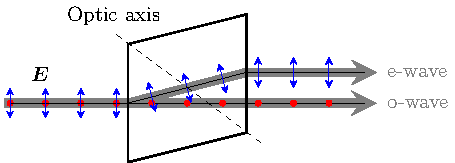
\includegraphics[scale=0.95]{images/theory/tikz_calcite_beams.pdf}
    \caption{The field components are separated as the light passes through the calcite crystal thereby forming the e- and o-wave. The components perpendicular to the optic axis shown as red dots pass through as expected for normal incidence, while the other components represented by the blue arrows are refracted. The component dependent spatial separation also explains why the polarization states of the two waves are orthogonal.}
    \label{fig:calcite_beams}
\end{figure}
%https://en.wikipedia.org/wiki/Optic_axis_of_a_crystal
Figure \ref{fig:uniaxial_source} shows the propagation of a wave emitted from an unpolarized source placed within a uniaxial crystal. The component of the field perpendicular to the optic axis will propagate with the same phase velocity $v_{\bot}$ in all directions, so that the wavefronts form the o-wave which further expands in the shape of a circle. Meanwhile the field component, which is not everywhere perpendicular to the optic axis, will be traveling with a phase velocity $v_{\parallel}$ in the directions perpendicular to the optic axis. The wavefronts of the e-wave therefore form an ellipse. We therefore end up with different refractive indices with extrema parallel and perpendicular to the optic axis. In this case the highest refractive index $n_o = \nicefrac{c}{v_{\bot}}$ is found in the directions parallel to the optic axis, while it is lowest for the perpendicular directions. As we can see from the figure $v_{\parallel} > v_{\bot}$ and since the refractive index perpendicular to the optic axis is given by $n_e = \nicefrac{c}{v_{\parallel}}$ it follows that $n_e < n_o$. With this it is possible to quantify the birefringent strength of the material via the difference $\Delta n = n_e - n_o$ in the refractive indices of the e- and o-wave. The difference $\Delta n$ is known as the birefringence of the material. Furthermore, if $\Delta n$ is negative then the crystal is said to be negative uniaxial which is the case for calcite and the example shown in figure \ref{fig:uniaxial_source}. Likewise, if $\Delta n$ is positive the material is positive uniaxial and in that case the ellipse formed by the wavefronts of the e-wave are enclosed within the circle formed by the wavefronts of the o-wave. 

\begin{figure}[h]
    \centering
    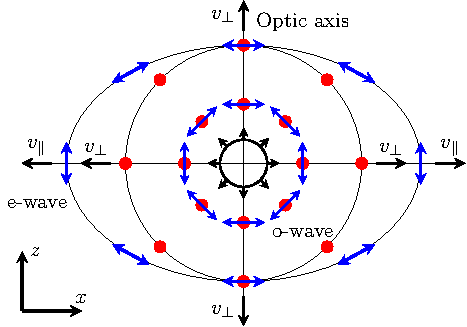
\includegraphics[scale=0.73]{images/theory/tikz_uniaxial_source.pdf}
    \caption{Cross section perpendicular to the optic axis of an unpolarized light source inside a uniaxial crystal. The red dots represent components which are everywhere perpendicular to the optic axis. They form the o-wave and expand in a circle because they experience the same refractive index everywhere. The components represented by the blue arrows are partly pointing in the direction of the optic axis. Therefore, depending on their orientation to the optic axis they experience a different refractive index so that the wavefront forms an ellipse.}
    \label{fig:uniaxial_source}
\end{figure}

For biaxial crystals the birefringence is still defined as the biggest difference between the refractive indices along the different directions. For completeness, it is worth mentioning the case in which the refractive indices along all the directions are equal. The unit cell of these materials is cubic causing them to be isotropic \cite{Hecht}. 
% TODO @JAN Move index ellipsoid+determining optic axis to appendix or remove completely 
Finally, to conclude this section we will give a description of the same situation but from another point of view. For this purpose we consider the energy density of an EM wave in an anisotropic medium.
We start by introducing a charge density $\rho$ and then express the work done by the fields moving it a distance $d\bm{l}=\bm{v}dt$ mathematically in terms of the field vectors. Since that gives us an idea of the energy stored in the fields. The force acting on the charge distribution is the Lorentz force density\footnote{The force density has the dimensions of force per volume and is needed so that when we integrate over the volume we get the total force.} $\bm{f}$:
\begin{equation}
    \bm{f}\cdot d\bm{l}=\rho(\bm{E}+\bm{v}\times\bm{B})\cdot\bm{v}dt=\rho\bm{E}\cdot\bm{v}dt
\end{equation}
We get the last equality because $\bm{v}\cdot(\bm{v}\times\bm{B})$ is zero for any $v$ and $\bm{B}$. 
If we then integrate over the volume $V$ enclosing the charge distribution and use the fact that $\bm{J}=\rho\bm{v}$ we get:
\begin{equation}
    \int_V \bm{f}\cdot d\bm{l} dV =\int_V \bm{E}\cdot\bm{J} dVdt
\end{equation}
since $\int_V \bm{f} dV = \bm{F}$ and $dW = \bm{F} d\bm{l}$ we finally end up with:
\begin{equation}
    \label{eq:emf_work}
    \frac{dW}{dt} = \int_V \bm{E}\cdot\bm{J} dV
\end{equation}
Since we want to express this in terms of the fields only, we use the Ampère-Maxwell law, that is equation \ref{eq:maxwell4}:
\begin{equation}
    \bm{J}\cdot\bm{E} = \frac{1}{\mu_0}\bm{E}\cdot(\bm{\nabla}\times\bm{B})-\bm{E}\cdot\frac{\partial\bm{D}}{\partial t}
\end{equation}
We can rewrite $\bm{E}\cdot(\bm{\nabla}\times\bm{B})$ as $-\bm{B}\cdot\frac{\partial \bm{B}}{\partial t} - \bm{\nabla}\cdot(\bm{E}\times\bm{B})$ using a product rule from vector calculus and the Maxwell–Faraday law (equation \ref{eq:maxwell3}). With the fact that $\bm{A}\cdot\frac{\partial \bm{A}}{\partial t} = \frac{1}{2} \frac{\partial A^2}{\partial t}$ for any vector $\bm{A}$ we end up with:
\begin{equation}
    \bm{J}\cdot\bm{E} = -\frac{1}{2}\frac{\partial}{\partial t}\left(\frac{1}{\mu_0}B^2+\bm{E}\cdot\bm{D}\right)-\frac{1}{\mu_0}\bm{\nabla}\cdot(\bm{E}\times\bm{B})
\end{equation}
which we then substitute back into equation \ref{eq:emf_work} and with the help of the divergence theorem we get:
\begin{equation}
    \label{eq:poyntings_theorem}
    \frac{dW}{dt} = -\frac{\partial}{\partial t} \int_V \frac{1}{2}\left(\frac{1}{\mu_0}B^2+\bm{E}\cdot\bm{D}\right)dV -\frac{1}{\mu_0}\oint_{\partial V} (\bm{E}\times\bm{B}) \cdot d\bm{s}
\end{equation}
This is known as Poynting's theorem in integral form and can be compared to the work-energy theorem of classical mechanics. That is, the work done by an electromagnetic force on a charge distribution equals the decrease of energy stored in the fields. The volume integral of equation \ref{eq:poyntings_theorem} is the total energy stored in the fields while the surface integral describes the energy flux or rate of transport out of the volume by the fields. We can therefore rewrite equation \ref{eq:poyntings_theorem} as:
\begin{equation}
    \frac{dW}{dt} = -\frac{\partial}{\partial t} \int_V u\, dV -\oint_{\partial V} \bm{S} \cdot d\bm{s}
\end{equation}
where we have set
\begin{equation}
    u = \frac{1}{2}\left(\frac{1}{\mu_0}B^2+\bm{E}\cdot\bm{D}\right),\; \bm{S} = \frac{1}{\mu_0}(\bm{E}\times\bm{B}),
\end{equation}
$u$ is the energy density of the fields and $\bm{S}$ is the energy flux density known as the Poyinting vector. Since we have no free charges for the cases considered in this work, that is free space or neutrally charged media, we set $\frac{dW}{dt}=0$. With equation \ref{eq:emf_work} we get the differential form:
\begin{equation}
    \label{eq:poynting_theorem_diff_form}
    \frac{\partial u}{\partial t} = -\bm{\nabla} \cdot \bm{S},
\end{equation}
because the volume integral (equation \ref{eq:emf_work}) is zero for any volume. We see that \ref{eq:poynting_theorem_diff_form} has the same shape as a continuity equation like the heat flow equation or the continuity equation in quantum mechanics related to the conservation of probability, in this case it shows that energy is conserved locally. Finally, if we take only the electric field contribution to the energy density, that is $u_e = \frac{1}{2}\bm{E}\cdot\bm{D}$, and choose a coordinate system in which the dielectric tensor is diagonal, known as the principal coordinate system, then we can write the electric displacement vectors for which $u_e$ is constant as:
\begin{equation}
    \frac{D_x^2}{\epsilon_x}+\frac{D_y^2}{\epsilon_y}+\frac{D_z^2}{\epsilon_z}= 2u_e
\end{equation}
where $\epsilon_x$, $\epsilon_y$ and $\epsilon_z$ are the dielectric constants on the diagonal of $\hat{\epsilon}$ called the principal dielectric constants. Additionally we scale $\bm{D}$ by $\nicefrac{1}{\sqrt{2u_e}}$, replace it with $\bm{r}$ and set $n_i^2 = \nicefrac{\epsilon_i}{\epsilon_0},\; (i=x,y,z)$. This gives us:
\begin{equation}
    \frac{x^2}{n_x^2}+\frac{y^2}{n_y^2}+\frac{z^2}{n_z^2}=1,
\end{equation}
which is the equation of an ellipsoid and is therefore called the index ellipsoid. In a uniaxial crystal two of the three principal dielectric constants are equal because of the symmetry plane oriented perpendicular to the optic axis. In that case the index ellipsoid reduces to:
\begin{equation}
    \label{eq:negative_index_ellipsod}
    \frac{x^2+y^2}{n_o^2}+\frac{z^2}{n_e^2}=1.
\end{equation}
Going back to figure \ref{fig:uniaxial_source} we see that the optic axis is along the z-axis and the xy-plane is perpendicular to it. According to convention the symmetry axis is chosen as the z-axis so that $n_x=n_y=n_o$ and $n_z=n_e$. The index ellipsoid can also be used to find the propagation directions of the e- and o-wave as well as the optic axis of a biaxial or uniaxial crystal given a wavevector $\bm{k}$. To do that $\bm{k}$ is placed at the center of the index ellipsoid. A plane normal to $\bm{k}$ is then drawn centered at the origin so that the intersection of the plane and the ellipsoid forms an ellipse. The semi-axes then show the directions of the e- and o-wave and their length is equal to $n_e$ and $n_o$. If the intersection forms a circle instead of an ellipse then it indicates that $\bm{k}$ is parallel to an optic axis, which is then the only optic axis in the case of a uniaxial medium \cite{Yariv1984, Griffiths2017}. 
In this section we discussed a physical model based on a classical mechanical description. It explains the observed phenomena of double refraction and the related effects. This model surely only works to some extent and a better model of the interaction between the EM fields and the charged particles requires a quantum mechanical description. However, as mentioned earlier the Lorentz model of the birefringence is sufficient for this work. We will see that birefringence does not only have its origin at the atomic level in the following section about form birefringence. 

Surprisingly it is also possible for a material to appear birefringent even though all sets of springs are equally stiff in the Lorentz oscillator model. A possible realization of such a material is an infinite medium consisting of alternating layers of two different homogeneous and isotropic media. Even though each individual layer is isotropic the structure as a whole acts as an anisotropic medium. It can be shown that field components parallel and perpendicular to the layering propagate at different speeds. This type of birefringence is called form birefringence. Even though it is of a different type, the ideas and principles of this section still apply, with the exception of the mechanism causing the birefringence. The derivation and explanation of form birefringence will be the focus of the next section which is based on the work by Rytov \cite{Rytov1956}. 

\subsection{Form birefringence}
\label{sec:form_birefringence}
Form birefringence has the interesting property that the birefringence can be controlled or tuned to some extend directly via the geometry of the medium. As mentioned in the previous subsection \ref{sec:wave_prop} in this subsection we will consider the propagation of an EM wave in a medium consisting of alternating layers. The material of each layer is homogeneous and isotropic with no other restrictions on the optical properties, i.e. the permittivity and permeability are scalars instead of tensors. According to Rytov's work, for sufficiently long wavelengths compared to the structural periodicity of the medium, the periodic layering will then appear anisotropic. So that it in the end is birefringent as well as dichroic if we take absorption into consideration. For each layer we set the refractive index of the layer material as $n_i^2 = \epsilon_i \mu_i$. As mentioned earlier the materials used for the applications in this work are actually non-magnetic, however to keep track of the constants we assign an index to the permeabilities of each layer, even though $\mu_1=\mu_2=\mu_0$. Additionally, we let the width of the layer with $\epsilon_1$ be $a$ and $b$ for the other layer. The derivation is fairly tedious but it is interesting since it shows which approximations and assumptions are made as well as how the wave actually propagates in the structure. The idea of the derivation is to calculate the average field strength over the width $a+b\equiv d$. Therefore the calculation only makes sense if the change of the field is small over a period $d$. This condition can be written as:
\begin{equation}
    \label{eq:rytov_cond1}
    kd|n|\ll 1,
\end{equation}
where n is the effective index of refraction. There are only three different directions in which the wave can propagate in the medium because of symmetry. That is any other direction is equivalent in the sense that it is either mirrored or a superposition of two of the three directions and the field can then be decomposed along those two directions. In two of the cases the wave propagates parallel to the layers and then either the magnetic or the electric field is parallel to the layers as well. In the third case the wave propagates perpendicular to the layers. One of the two cases for parallel propagation is shown in \ref{fig:tikz_rytov_derivation}. This is the geometry that is relevant for the applications we discuss in this work, that is one of the electric field components is perpendicular to the layering and one is parallel. 

\begin{figure}[h]
    \centering
    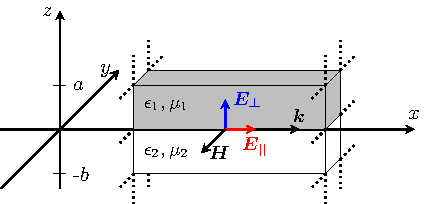
\includegraphics[scale=1.5]{images/theory/tikz_rytov_derivation.pdf}
    \caption{Infinite finely stratified medium. The medium consists of two isotropic and homogeneous material layers with dielectric constants and permeabilities $\epsilon_1, \mu_1$ (width a) and $\epsilon_2, \mu_2$ (width b). Here we consider the case for a wave propagating parallel to the layers along the x-axis so that one component of the electric field is perpendicular to the layering and the other one is parallel.}
    \label{fig:tikz_rytov_derivation}
\end{figure}

We set the z-axis perpendicular to the layers so that $\bm{k}$ and $\hat{\bm{e}}_z$ are perpendicular. For this case the electric field has two components and the magnetic has one: $\bm{E}=\bm{E_{\bot}} + \bm{E_{\parallel}} = E_x \hat{\bm{e}}_x + E_{z} \hat{\bm{e}}_z$ and $\bm{H}=H_y=H \hat{\bm{e}}_y$. That is we set the y- and z-axis along the directions of $\bm{H}$ and $\bm{E_{\bot}}$ respectively. Again, we start from Maxwell's equations. We use Ampère's law (equation \ref{eq:maxwell3}) and Faraday's law of induction (equation \ref{eq:maxwell4}). Again there are no free charges or currents although now we have that $\bm{B} = \hat{\mu} \bm{H}$. The equations transformed into k-space $(\partial_t \xrightarrow{\mathscr{F}} ik)$ are:
\begin{equation}
    \label{eq:rytov_maxwell_initial}
    \bm{\nabla}\times\bm{E} =-ik \hat{\mu} \bm{H},
    \qquad
    \bm{\nabla}\times\bm{H} = ik \hat{\epsilon} \bm{E}.
\end{equation}

We substitute in the fields and use the fact that both materials are isotropic. This gives us three equations for the field components:
\begin{equation}
    \label{eq:rytov_maxwell}
    \partial_z E_x - \partial_x E_z = - ik \mu H,
    \qquad
    \partial_x H = ik \epsilon E_z,
    \qquad
    \partial_z H = -ik \epsilon E_x.
\end{equation}
Necessarily, since the structure of the material is periodic $\epsilon$ and $\mu$ must be periodic as well. Therefore the solution to the equations in \ref{eq:rytov_maxwell} must be periodic too in $z$ with a period $d$ so a good guess are plane waves:
\begin{equation}
    \label{eq:rytov_field_ansatz}
    H = U(z)e^{-iknx},
    \qquad
    E_x = V(z)e^{-iknx},
    \qquad
    E_z = W(z)e^{-iknx},
\end{equation}
which we substitute into equation \ref{eq:rytov_maxwell} to get a set of equations connecting the amplitudes:
\begin{equation}
    \partial_z V + iknW = -ikn \mu U,
    \qquad
    -Un = \epsilon W,
    \qquad
    \partial_z U = ik \epsilon V.
\end{equation}
For this set of equations there exists analytical solutions:
\begin{align}
\begin{split}
    \label{eq:rytov_amplitudes}
    U=A_j\cos \alpha_jz + B_j\cos \alpha_j & z, 
    \qquad
    V=\frac{-\alpha_j}{ik\epsilon_j}(A_j\sin \alpha_j z -B_j\cos \alpha_j z ),
    \\
    &W=\frac{n}{\epsilon_j}U,
\end{split}
\end{align}
where $\alpha_j = k \sqrt{\epsilon_j\mu_j-n^2}$ and $j$ is 1 $\text{if $z \bmod d \in [0, a)$}$ else $2$. The field components parallel to the layers must be continuous at the interfaces. This implies that the components have to be periodic, since e.g. the interface at $0$ is indistinguishable from the one at $a$. Furthermore, the same conditions apply to the amplitudes because of equation \ref{eq:rytov_field_ansatz}, that is they must be equal at the interfaces $\pm 0$ and $a, -b$:
\begin{align}
\begin{split}
    U(+0) = U(-0), 
    \qquad
    &V(+0) = V(-0),
    \\
    U(a-0) = U(-b+0),
    \qquad
    &V(a-0) = V(-b+0),
\end{split}
\end{align}
where the signs indicate the directions of the limits. We substitute the amplitudes (equation \ref{eq:rytov_amplitudes}) in these boundary conditions so that we get four equations determining the coefficients $A_1,A_2,B_1$ and $B_2$:
\begin{align}
\begin{split}
    \label{eq:rytov_waves}
    A_2 = A_1, 
    \quad
    &A_2\cos \alpha_2 b - B_2 \sin \alpha_2 b= A_1 \cos \alpha_1 a + B_1 \sin \alpha_1 a,
    \\
    B_2=\beta B_1,
    \quad
    &A_2 \sin \alpha_2 b + B_2 \cos \alpha_2 b = -\beta (A_1 \sin \alpha_1 a - B_1 \cos \alpha_1 a),
\end{split}
\end{align}
where $\beta = \frac{\epsilon_2 \alpha_1}{\epsilon_1 \alpha_2}$. A homogeneous system of equations has infinitely many solutions if its determinant is zero. This is the interesting case since otherwise we would be left with the trivial solution only. 
\begin{equation}
   0\overset{!}{=}
   \begin{vmatrix} 
   1 & 0 & -1 & 0 \\
   \cos \alpha_1 a & -\sin \alpha_1 a & \cos \alpha_2 b & -\sin \alpha_2 b \\
   0 & -\beta & 0 & 1 \\
   \beta \sin \alpha_1 a & -\beta \cos \alpha_1 a & \sin \alpha_2 b & \cos \alpha_2 b \\
   \end{vmatrix} 
\end{equation}
calculating this determinant we see that:
\begin{equation}
    (1+\beta^2) \sin \alpha_1 a \sin \alpha_2 b + 2\beta (1-\cos \alpha_1 a \cos \alpha_2 b) = 0,
\end{equation}
i.e. a dispersion relation since $\alpha$ is a function of $n$ and $k$. This equation is quadratic in $\beta$ so we end up with two solutions $\beta_1$ and $\beta_2$:
\begin{equation}
    \beta_1 = -\frac{\tan \frac{\alpha_2 b}{2}}{\tan \frac{\alpha_1 a}{2}},
    \qquad
    \beta_2 = -\frac{\tan \frac{\alpha_1a}{2}}{\tan \frac{\alpha_2 b}{2}}.
\end{equation}
The question is which of these two solutions are of physical interest. To answer that we calculate the mean of the field components over the period $d$ and tryout each of the two possible values for $\beta$. To calculate the mean values we have to split the integral over the full width $d$ into two; one where $z$ goes from $0$ to $a$ and one from $0$ to $-b$. Together with equation \ref{eq:rytov_waves} we can then calculate the ratios of the means which simplifies the expressions. Specifically, we compare the mean field of the perpendicular component to the two parallel mean fields:
\begin{equation}
    \label{eq:rytov_mean_ratios}
    \frac{\overline{U}}{\overline{W}} = \frac{\overline{H}}{\overline{E_z}} = \frac{\epsilon_1 \alpha_2^2 - \epsilon_2 \alpha_1^2}{n\left(\alpha_2^2-\alpha_1^2 \right)},
    \qquad
    \frac{\overline{V}}{\overline{W}} = \frac{\overline{E_x}}{\overline{E_z}} = \frac{\epsilon_1^{-1} - \epsilon_2^{-1}}{k^2\left(\alpha_1^{-2} - \alpha_2^{-2} \right)}P,
\end{equation}
with
\begin{equation}
    P = \frac{U(a-0)-U(+0)}{V(a-0)-V(+0)} = -\frac{ik\epsilon_1}{\alpha_1}\frac{1}{\tan \frac{\alpha_2 b}{2}}\frac{\beta \tan \frac{\alpha_1 a}{2} + \tan \frac{\alpha_2 b}{2}}{\beta \tan \frac{\alpha_2 b}{2} + \tan \frac{\alpha_1 a}{2}}.
\end{equation}
We see that depending on which solution we choose the last factor of $P$ is either $0$ or tends to infinity. Furthermore, if $\beta = \beta_1$ is chosen then because of equation \ref{eq:rytov_mean_ratios} $\overline{E_x}$ is $0$. In that case the mean field is a transverse wave. For $\beta = \beta_2$ it is possible to show that $E_z$ and $H$ are odd functions and $E_x$ is even around the middle of each layer. The mean of $E_z$ and $H$ therefore vanishes and only $E_x$ is left. But $E_z$ and $B$ are odd and so the fields are $0$ in the middle of each layer. This situation is similar to a rectangular waveguide in the sense that the parallel component of the electric field and the normal component of the magnetic field is $0$ at the inner walls. This means that waves with frequencies below the cutoff frequency will be exponentially attenuated and will not propagate far. Since we assume that the wavelength must be greater than the period $d$ (equation \ref{eq:rytov_cond1}) it follows that the frequency is below the cutoff frequency. Consequently, waves for which $\beta = \beta_2$ will not propagate far and therefore $\beta = \beta_1$. The mean fields also satisfy equations \ref{eq:rytov_maxwell} but without the field component along the x-axis:
\begin{equation}
    \label{eq:rytov_maxwell_reduced}
    \partial_x \overline{H} = ik \epsilon_e \overline{E_z},
    \qquad
    \partial_x \overline{E_z} = ik \mu_e \overline{H},
\end{equation}
where $\epsilon_e \mu_e =n^2$ is the effective permittivity of the layers. Substituting in the mean fields we get:
\begin{equation}
    \left(\frac{\overline{U}}{\overline{W}}\right)^2 = \frac{\mu_e}{\epsilon_e}, 
\end{equation} so that with equation \ref{eq:rytov_mean_ratios} we obtain an expression for the effective permittivity and permeability:
\begin{equation}
    \epsilon_e = \frac{\epsilon_1 \alpha_2^2 - \epsilon_2 \alpha_1^2}{\alpha_2^2-\alpha_1^2},
    \qquad
    \mu_e = n^2\frac{\alpha_2^2-\alpha_1^2}{\epsilon_1 \alpha_2^2 - \epsilon_2 \alpha_1^2},
\end{equation}
where $n$ is determined by the first root ($\beta_1$) of the dispersion relation:
\begin{equation}
    \label{eq:rytov_n}
    \frac{\alpha_2}{\epsilon_2}\tan \frac{\alpha_2 b}{2} = -\frac{\alpha_1}{\epsilon_1}\tan \frac{\alpha_1 a}{2}.    
\end{equation}
This would be a good place to stop and use the previous result to determine $n$ but that is easier said than done. The problem is that \ref{eq:rytov_n} is a transcendental equation which often are not solvable in closed form, like in this case. That is also why equation \ref{eq:rytov_cond1} cannot be written in a more explicit form by solving equation \ref{eq:rytov_n} for $n$. There are of course numerical methods which can be used to calculate the roots but that approach introduces other practical issues. A way of dealing with this is by approximating the tangent function by its Taylor series around the origin. Since the error of this approximation increases for larger arguments we require that the arguments of the tangent functions are small:
\begin{equation}
    |\alpha_1 a| \ll 1, 
    \qquad
    |\alpha_1 b| \ll 1.
\end{equation}
It follows from the definition of $\alpha$ that the wavelength must be large compared to $a$ and $b$. The first three terms of the Taylor series are: $\tan x \approx x + \frac{1}{3}x^3 + \frac{2}{15}x^5 + ...$ The first order approximation is therefore obtained by simply replacing tangent by its argument. Solving for $n$ and using $n=\sqrt{\epsilon_e \mu_e}$ we end up with the following first order approximation:
\begin{equation}
    \label{eq:rytov_1st_order}
    \epsilon_{e,0} = \frac{\epsilon_1 \epsilon_2 (a+b)}{a\epsilon_2+b\epsilon_1},
    \qquad
    \mu_{e,0} = \frac{a\mu_1+b\mu_2}{a+b}.
\end{equation}
If we include the second order terms in the expression the approximation results in:
\begin{align}
\begin{split}
    \label{eq:rytov_2nd_order}
    \epsilon_{e} &= \epsilon_{e,0} + \frac{k^2a^2b^2}{12d^2} \frac{a\epsilon_1+b\epsilon_2}{(a+b)\epsilon_1^2\epsilon_2^2}\left(n_1^2-n_2^2\right)\left(\epsilon_1-\epsilon_2\right)\epsilon_{e,0}^3,
    \\
    \mu_{e} &= \mu_{e,0} + \frac{k^2a^2b^2}{12d^2}\frac{a\epsilon_1 + b\epsilon_2}{a\epsilon_2 + b\epsilon_1}\left(n_1^2-n_2^2\right)\left(\mu_1-\mu_2\right).
\end{split}
\end{align}
The $x^5$ term becomes too difficult to solve for $n$, so this is a good place to stop the expansion. The expressions as they are given in equation \ref{eq:rytov_2nd_order} are not directly applicable to the geometries and devices discussed later in this work. Like the geometry we just discussed the structure of the present devices are also layered, but the fields in question have field components parallel and perpendicular to the layering. This geometry is shown in figure \ref{fig:stratified_structure} where the electric field has components $E_{\bot}$ and $E_{\parallel}$ which are respectively perpendicular and parallel to the layering. The geometries shown in figure \ref{fig:tikz_rytov_derivation} and \ref{fig:stratified_structure} are equivalent except that the former has been rotated by $\SI{-90}{\degree}$ around the y-axis. 

\begin{figure}[h]
    \centering
    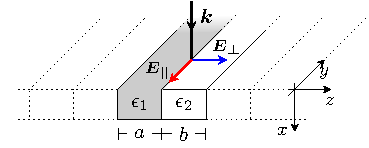
\includegraphics[scale=2]{images/theory/tikz_stratified_structure.pdf}
    \caption{The same structure as is shown in figure \ref{fig:tikz_rytov_derivation} but from a different point of view and in this case the material is non-magnetic. In this figure the structure is rotated by $\SI{-90}{\degree}$ around the y-axis. In general the electric field has two components parallel to the yz-plane at normal incidence. They can be decomposed into a perpendicular and parallel component. This is useful since the effective permittivity is known along those two directions. The magnetic field vector is not shown since we are only interested in the electric field.}
    \label{fig:stratified_structure}
\end{figure}

We can take any field propagating parallel to the x-axis and decompose it into a component parallel and perpendicular to the layering. Now, since Maxwell's equations are symmetric under the interchange of the electric and magnetic field in regions without free charge or currents, we can go back to the start of the derivation and apply the following transformation: $(\bm{H},\bm{E},\hat{\epsilon},\hat{\mu}) \rightarrow (\bm{E},\bm{-H},\hat{\mu},\hat{\epsilon})$. The derivation and the equations are still valid with this replacement. By doing this we quickly get an expression for the effective permittivity in the direction parallel to the layers. Specifically, we simply replace $\mu_i$ with $\epsilon_i$ and vice versa in equations \ref{eq:rytov_1st_order} and \ref{eq:rytov_2nd_order}. This is also the reason why we assigned each layer a permeability different from $\mu_0$. Finally, because Maxwell's equations are linear it follows that a superposition of two valid solutions is again a valid solution. Using this fact while actually setting $\mu_1=\mu_2=\mu_0$ and then carrying out the replacement described above we obtain an expression for the approximate effective permittivities of the parallel and perpendicular field components:
\begin{align}
\begin{split}
    \label{eq:rytov_2nd_order_final}
    \epsilon_{s} &= \tilde{\epsilon}_{s} + \frac{k^2a^2b^2}{12d^2} \frac{a\epsilon_1+b\epsilon_2}{(a+b)\epsilon_1^2\epsilon_2^2}\left(n_1^2-n_2^2\right)\left(\epsilon_1-\epsilon_2\right){\tilde{\epsilon}_{s}}^3,
    \\
    \epsilon_{p} &= \tilde{\epsilon}_{p} + \frac{k^2a^2b^2}{12d^2}\left(n_1^2-n_2^2\right)\left(\epsilon_1-\epsilon_2\right),
\end{split}
\end{align}
with the first order terms:
\begin{equation}
    \label{eq:rytov_1st_order_final}
    \tilde{\epsilon}_{s} = \frac{\epsilon_1 \epsilon_2 (a+b)}{a\epsilon_2+b\epsilon_1},
    \qquad
    \tilde{\epsilon}_{p} = \frac{a\epsilon_1+b\epsilon_2}{a+b},
\end{equation}
where $s$ and $p$ indicate the perpendicular and parallel directions respectively. If not stated otherwise then equations \ref{eq:rytov_2nd_order_final} and \ref{eq:rytov_1st_order_final} are used throughout this work to calculate the birefringence in the case of form birefringent materials. Additionally, we see that Maxwell's equations at the start of the derivation in this section as well as the boundary conditions are invariant under rotations of the geometry around the z-axis. This means that equations \ref{eq:rytov_2nd_order_final} and \ref{eq:rytov_1st_order_final} are invariant under such rotations as well. The optic axis must therefore be along the z-direction. Furthermore, this means that the effective permeability is $\epsilon_{p}$ throughout the whole xy-plane. Therefore the structure has one optic axis which makes it uniaxial. Moreover, we can write the dielectric tensor in the principal coordinate system of the geometry as follows:
\begin{equation}
    \label{eq:rytov_tensor}
    \hat{\epsilon} = 
    \begin{pmatrix}
        \epsilon_{p} & 0 & 0 \\
        0 & \epsilon_{p} & 0 \\
        0 & 0 & \epsilon_{s} \\
    \end{pmatrix}
\end{equation}
The question is though whether the structure is positive or negative uniaxial. To answer this we need to determine if $n_{s} < n_{p}$. Since the permittivities of the individual layers are complex numbers or rather complex functions the effective permittivities are as well and therefore also the refractive indices. Hence, for the inequality to make sense we only compare the real parts of the refractive indices. To this end we therefore set $(n_r+in_i)^2 \overset{!}{=} \epsilon_r + i\epsilon_i$ where the subscripts $i$ and $r$ indicate the real and imaginary parts respectively. Comparing the coefficients then gives us expressions for the real and imaginary parts of the refractive index:
\begin{equation}
    n_r = \sqrt{\frac{|\epsilon|+\epsilon_r}{2}}, 
    \qquad 
    n_i = \sqrt{\frac{|\epsilon|-\epsilon_r}{2}},
\end{equation}
where $|\cdot|$ denotes the magnitude. The birefringence is therefore given by:
\begin{equation}
    \label{eq:form_bf}
    \Delta n = \operatorname{Re}(n_e) - \operatorname{Re}(n_o) = \sqrt{\frac{|\epsilon_s|+\operatorname{Re}(\epsilon_s)}{2}} - \sqrt{\frac{|\epsilon_p|+\operatorname{Re}(\epsilon_p)}{2}}.
\end{equation}
Similarly we can define the dichroism $\Delta \kappa$ as the difference of the imaginary parts:
\begin{equation}
    \Delta \kappa = \operatorname{Im}(n_s) - \operatorname{Im}(n_p) = \sqrt{\frac{|\epsilon_s|-\operatorname{Re}(\epsilon_s)}{2}} - \sqrt{\frac{|\epsilon_p|-\operatorname{Re}(\epsilon_p)}{2}}.
\end{equation}

Furthermore, in the case of $\epsilon_r^2 \gg \epsilon_i^2$ the refractive index is approximately given by $n^2 \approx \epsilon_r$. It is therefore sufficient to determine if $\epsilon_{s} < \epsilon_{p}$. It is fairly straight forward to show that this inequality is true for the first order, even for arbitrary parameters. For the second order we need to make some reasonable restrictions on the values of the parameters to obtain an answer independent of the value domain. Specifically, the layering of the structures with which we are concerned in this work are alternating air or dielectric. The real part of the permittivity of the dielectric is assumed to be lower than four, which is the case for the materials used in this work. With this it is possible to show that $\epsilon_{s} < \epsilon_{p}$ is true for the second order approximation as well. This is shown in section \ref{sec:bf_proof} of the appendix. If we go back to figure \ref{fig:uniaxial_source} we see that the field component polarized in the direction of the optic axis forms the e-wave which is along the z-axis. Therefore, the e-wave experiences an effective permittivity of $\epsilon_{s}(=\epsilon_{e})$. Analogously, the effective permittivity of the o-wave is $\epsilon_{p}(=\epsilon_{o})$. Since $\epsilon_{s} < \epsilon_{p}$ we can finally conclude that the structure is negative uniaxial, i.e. $n_e < n_o$. Additionally, figure \ref{fig:uniaxial_source} shows that along these two directions the birefringence is maximal. 

Finally this means that we can write the equation describing the index ellipsoid as:
\begin{equation}
    \frac{x^2+y^2}{n_p^2}+\frac{z^2}{n_s^2}=1.
\end{equation}
The shape of this ellipsoid is shown in figure \ref{fig:index_ellipse}. Since the wave propagates along the x-direction we draw an ellipse intersecting the ellipsoid in the yz-plane. Again we see that the two indices of refraction of the electric field components in this direction are $n_{p}$ and $n_{s}$. 
\begin{figure}[h]
    \centering
    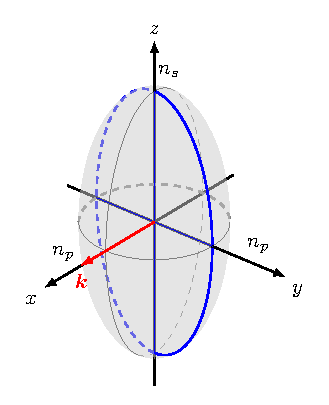
\includegraphics[scale=1]{images/theory/tikz_index_ellipse.pdf}
    \caption{Index ellipsoid of the stratified structure shown in figure \ref{fig:stratified_structure}. $\bm{k}$ indicates the direction of propagation. The blue ellipse is perpendicular to this direction and can be used to find the two indices of refraction of the wave; in this case $n_{p}$ and $n_{s}$.}
    \label{fig:index_ellipse}
\end{figure}

In summary, we considered the propagation of an EM wave in an evenly layered medium. To that extend we went through the derivation of an equation for the mean field effective refractive index. Since we considered the spatial average of the field for this derivation, the result is only valid in the case of waves which are long relative to the structural period. I.e. the field variation has to be small compared to the period in order to justify using the mean field. The resulting equation does not in general permit an expression of the effective refractive index in terms of the widths and optical parameters of the layers. Following, a Taylor expansion is carried out and approximate expressions are obtained for the effective permittivities of the mean field components. With these expressions the birefringence of the structure can be approximated, where the error of the approximation increases for increasing wavelength. Furthermore, we saw that the stratified structures with which we are concerned appear uniaxial. In total, we considered propagation within the stratified medium only, following the next section will be about what happens at the boundary between two media with different dielectric tensors.

% TODO @JAN You don't have to read this.
%I'm not sure wether to keep it or not. I don't really use it. It's almost like the Fresnel equations anyways. Don't know ... Dump it into the appendix?
% (if removed rewrite last sentence of previous part, move ending of this part) 
\subsection{Interface conditions}
\label{sec:interface_conditions}
The previous section answered the question about how each field component propagates inside the stratified medium in the case of long waves. The question that still remains is what happens with the wave as it enters the medium. There are three cases: Either one medium is isotropic and one is anisotropic or in the second case both media are anisotropic. The third case is less interesting since it is already described by the Fresnel equations. Furthermore, we will only consider the case of normal incidence, since that is given by the geometry of the measurements in this work. We do not have to consider double refraction since we know that the o-wave travels at the same speed in every direction as if the medium was isotropic. The o-wave therefore obeys Snell's Law and will not be refracted at normal incidence. Similarly, since the e-wave is everywhere parallel to the optic axis it will also effectively experience an isotropic medium and the refraction can therefore be described by Snell's Law. In contrast to the calcite crystal example described in section \ref{sec:wave_prop} we will therefore not get two spatially separated waves. However, we will still get a reflected wave. In the case of an interface between two isotropic materials we could use the Fresnel equations but since the material in this case appears anisotropic we have to take this into account in the derivation of the transmission and reflection coefficients. The geometry is shown in figure \ref{fig:interface_derivation} where the wave ($\bm{k_i}$) is normally incident on the interface between two anisotropic media. According to the wave equation we will in general get a reflected ($\bm{k_r}$) and a transmitted wave ($\bm{k_t}$). 

\begin{figure}[h]
    \centering
    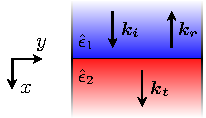
\includegraphics[scale=2.7]{images/theory/tikz_interface_derivation.pdf}
    \caption{A wave with wavevector $\bm{k_i}$ which is normally incident on the boundary between two anisotropic media. The wave propagates along the x-direction. The general solution to the wave equation allows a wave propagating in both positive and negative x-direction; a transmitted and reflected wave with wavevectors $\bm{k_t}$ and $\bm{k_r}$ respectively.}
    \label{fig:interface_derivation}
\end{figure}

To begin with, we derive conditions relating the parallel and normal field components at both sides of any neutrally charged non-conducting interface. These conditions will be useful for the calculation of the reflection and transmissions coefficients at the interface between two anisotropic media. Once more we start with Maxwell's equations (\ref{eq:maxwell1reduced}-\ref{eq:maxwell4reduced}) specifically Faraday's law of induction:
\begin{equation}
    \bm{\nabla}\times\bm{E} =-\frac{\partial\bm{B}}{\partial t}.
\end{equation}
Using Stokes' theorem can quickly obtain Faraday's law in integral form:
\begin{equation}
    \label{eq:int_faradays_law}
    \int_A \bm{\nabla}\times\bm{E}\cdot d\bm{A} = \oint_{\delta A} \bm{E}\cdot d \bm{l} = -\int_A \frac{\partial\bm{B}}{\partial t}\cdot d\bm{A},
\end{equation}
where $\delta A$ is the boundary of the area $A$. We set this surface $A$ in the plane of incidence, in this case the xy-plane, so that one half is in medium one and the other in medium two. If we let the sides perpendicular to the interface of area $A$ go to zero then the total area will go to zero and the right hand side of equation \ref{eq:int_faradays_law} will end up as zero. With this we therefore get that:
\begin{equation}
    \int_{l_{1,t}} E_{1,t} dl - \int_{l_{2,t}} E_{2,t} dl = 0,
\end{equation}
where the $t$ subscript denotes the field components and paths tangential to both sides of the interface. Since  we did not choose any specific interface or electric field we can omit the integration. This gives us the continuity condition for the tangential components of the electric field at the interface:
\begin{equation}
    \label{eq:t_boundary_cond_e}
    \bm{n} \times (\bm{E_1} - \bm{E_2}) = 0,
\end{equation}
where $\bm{n}$ is normal to the interface, $\bm{E_1}$ and $\bm{E_2}$ are the electric fields in medium one and two respectively. Furthermore, since we have no free currents and the materials are non-magnetic we can derive a condition for the tangential components of the magnetic field in a similar manner. We use Ampère's circuital law (\ref{eq:maxwell4reduced}) which we write it in integral form. Subsequently we shrink the integration area around the interface. This yields:
\begin{equation}
    \label{eq:t_boundary_cond_b}
    \bm{n} \times (\bm{B_1} - \bm{B_2}) = 0,
\end{equation}
where $\bm{B_1}$ and $\bm{B_2}$ are the magnetic fields in medium one and two respectively.
Again, to obtain interface conditions for the normal components of the fields we apply the same procedure. We start with Gauss's law for magnetism $(\bm{\nabla}\cdot \bm{B} = 0)$. If we integrate over a volume enclosing the interface, and then shrink this volume we get a condition for the normal component of the magnetic field at the boundary:
\begin{equation}
    \label{eq:n_boundary_cond_b}
    \bm{n}\cdot(\bm{B_1}-\bm{B_2}) = 0.
\end{equation}
I.e. the normal component of the magnetic field is continuous across the interface. The final general condition, obtained in a similar manner, is the condition that the normal component of the displacement field $\bm{D}$ is continuous across the interface. Which can be expressed as:
\begin{equation}
    \label{eq:n_boundary_cond_d}
    \bm{n}\cdot(\bm{D_1}-\bm{D_2}) = 0,
\end{equation}
where $\bm{D_1}$ and $\bm{D_2}$ are the displacement fields at each side of the interface \cite{Destriau1949, Griffiths2017}. Specifically, in the context of this work we are interested in the reflection and transmission coefficients of the interface between two periodically stratified media 1 and 2. In the previous section $\ref{sec:wave_prop}$ about form birefringence we derived approximations for the dielectric tensors of such periodic media given the individual layer material and thickness. Additionally, in the case we consider the two anisotropic media on each side of the interface are rotated at some angles $\alpha_1$ and $\alpha_2$ around a common x-axis. This means that in a third system the dielectric tensors of both media given by equation \ref{eq:rytov_tensor} will not be diagonal. We could use the principal coordinate system of one media but since there in general are multiple interfaces we instead use a lab system as the reference system. This system is the one shown in figure \ref{fig:interface_derivation}. The plane of incidence is therefore the xy-plane and the interface lies in the yz-plane, parallel to the layering. In the lab system $\hat{\epsilon}$ is given by:
\begin{equation}
    \label{eq:lab_epsilon}
    \hat{\epsilon_i}(\alpha_i) = \hat{R}_x(\alpha_i) \hat{\epsilon_i}' \hat{R}_x(-\alpha_i),
\end{equation}
where $\hat{\epsilon_i}'$ is the dielectric tensor in its principal coordinate system, $i=1,2$ and $\hat{R}_x(\alpha_i)$ rotates a vector around the x-axis by an angle $\alpha_i$. $\hat{R}_x(\alpha_i)$ can be represented as:
\begin{equation}
    \label{eq:x_rotation_matrix}
    \hat{R}_x(\alpha_i) = 
    \begin{pmatrix}
        1 & 0 & 0 \\
        0 & \cos (\alpha_i) & -\sin (\alpha_i) \\
        0 & \sin (\alpha_i) & \cos (\alpha_i) \\
    \end{pmatrix}
\end{equation}
\cite{J.Muthsam2006}.
For clarification, the dielectric tensors of media 1 and 2 are different not only because of the different angles $\alpha_i$ but also because of different diagonal entries, e.g $\epsilon_{p,1} \neq \epsilon_{p,2}$. With this description of the setup we can proceed with the derivation of the reflection and transmission amplitudes. Respectively, we can represent the incident, reflected and transmitted electric field as follows:
\begin{align}
\begin{split}
    \bm{E_i} = \bm{E}_{0,i}e^{i(\bm{k}_i\bm{r}-\omega_i t)},
    \quad
    \bm{E_r} = \bm{E}_{0,r}e^{i(\bm{k}_r\bm{r}-\omega_r t)},
    \quad
    \bm{E_t} = \bm{E}_{0,t}e^{i(\bm{k}_t\bm{r}-\omega_t t)}.
\end{split}
\end{align}
We get similar expressions for the magnetic field, simply by replacing $E$ with $B$. 
The boundary conditions on the interface that the tangential components of the electric and magnetic field are continuous, i.e. equations \ref{eq:t_boundary_cond_e} and \ref{eq:t_boundary_cond_b}, requires that
\begin{align}
\begin{split}
    \label{eq:field_conditions}
    \bm{k}_i \cdot \bm{r} = \bm{k}_r \cdot& \bm{r} = \bm{k}_t \cdot \bm{r}, \\
    \omega_i = \omega_r& = \omega_t,
\end{split}
\end{align}
\begin{align}
\begin{split}
    \label{eq:interface_amplitudes}
    \bm{n} \times (\bm{E}_{i} + \bm{E}_{r}) = \bm{n} \times \bm{E}_{t}, \\
    \bm{n} \times (\bm{B}_{i} + \bm{B}_{r}) = \bm{n} \times \bm{B}_{t}, \\
\end{split}
\end{align}
because all exponents must be equal for any $\bm{r}$ and $t$. The number of expressions in equation \ref{eq:field_conditions} show that conditions \ref{eq:t_boundary_cond_e} and \ref{eq:t_boundary_cond_b} are quite strong. Furthermore, since the wavevectors are given as:
\begin{equation}
    \bm{k}_i = k_{x,i} \bm{n}, \qquad \bm{k}_r = -k_{x,i} \bm{n} \qquad \bm{k}_t = k_{x,t} \bm{n},
\end{equation}
it follows that:
\begin{align}
\begin{split}
    &k_{x,i} = k_{x,r} = k = \sqrt{\hat{\epsilon}_{p,1}}\frac{\omega}{c}, \\
    &k_{x,t} = k_t = \sqrt{\hat{\epsilon}_{p,2}}\frac{\omega}{c}.
\end{split}
\end{align}
The last equation arises from the fact that the rotation is around the x-axis. Equation \ref{eq:lab_epsilon} also shows this; there is a mismatch between the permittivities of the two media along the x-axis. With Faraday's law we can obtain a system of equations relating the electric and magnetic fields of the incident, reflected and transmitted wave:
\begin{equation}
    \label{eq:some_equation}
    \bm{n} \times \bm{B}_i = -\frac{\omega}{k} \hat{\epsilon}_1 \bm{E}_i, \qquad
    \bm{n} \times \bm{B}_r = \frac{\omega}{k} \hat{\epsilon}_1 \bm{E}_r, \qquad
    \bm{n} \times \bm{B}_t = -\frac{\omega}{k_t} \hat{\epsilon}_2 \bm{E}_t.
\end{equation}
If we add the first two expressions of equation \ref{eq:some_equation} and use the fact that the tangential component of the magnetic field is continuous across the interface (equation \ref{eq:interface_amplitudes}) we get:
\begin{equation}
    \bm{n} \times \bm{B}_t = -\frac{\omega}{k}\hat{\epsilon}_1(\bm{E}_{i}-\bm{E}_{r}).
\end{equation}
With the last expression of equation \ref{eq:some_equation} we can eliminate the magnetic field in the previous expression:
\begin{equation}
    \label{eq:electric_field_eq}
    \frac{\omega}{k_t}\hat{\epsilon}_2 \bm{E}_t = \frac{\omega}{k}\hat{\epsilon}_1(\bm{E}_{i}-\bm{E}_{r}).
\end{equation}
Or if we set $n_{p,i} = \sqrt{\epsilon_{p,i}}$ then we can rewrite equation \ref{eq:electric_field_eq} as:
\begin{equation}
    \label{eq:electric_field_eq_rew}
    \frac{n_{p,1}}{n_{p,2}}\hat{\epsilon}_2 \bm{E}_t = \hat{\epsilon}_1(\bm{E}_{i}-\bm{E}_{r}).
\end{equation}

Finally, if we pair the interface condition for the tangential component of the electric field with equation \ref{eq:electric_field_eq} we obtain a homogeneous linear system of equations in the electric field components. These equations can be reduced to expressions which relate the incident electric field amplitudes to the reflected and transmitted amplitudes. Furthermore, we know from the previous section \ref{sec:wave_prop} that the field components along the direction of propagation are extinguished, i.e. a TEM wave. This means that we can omit the x-components in the expressions. With this we can write the relation between the incident and reflected field as:
\begin{equation}
    \label{eq:reflection_general}
    \bm{E_r} = \hat{T}_r \bm{E_i} =
    \frac{-1}{d}
    \begin{pmatrix}
        b_-b_+ - c_+a_- & c_-b_+ - c_+b_- \\
        b_+a_- - a_+b_- & b_+b_- - a_+c_- \\
    \end{pmatrix}
    \bm{E_i},
\end{equation}
we get a similar relation between the incident and transmitted field:
\begin{equation}
    \label{eq:transmission_general}
    \bm{E_t} = \hat{T}_t \bm{E_i} =
    \frac{2}{d}
    \begin{pmatrix}
        a_1c_+ - b_1b_+ & b_1c_+ - c_1b_+ \\
        b_1a_+ - a_1b_+ & c_1a_+ - b_1b_+ \\
    \end{pmatrix}
    \bm{E_i},
\end{equation}
where $a_i=\cos^2(\alpha_i)\epsilon_{p,i}+\sin^2(\alpha_i)\epsilon_{s,i}$, $b_i=\frac{1}{2}\sin(2\alpha_i)(\epsilon_{p,i}-\epsilon_{s,i})$, $c_i = a_i(\alpha_i + \nicefrac{\pi}{2})$ with $i=1,2$ for medium 1 and 2 respectively, $x_{\pm}=x_1\pm \frac{n_{p,1}}{n_{p,2}} x_2, x=a,b,c$ and finally $d=a_+c_+-b_+b_+$. We can consider special cases to check the plausibility of the two expressions \ref{eq:transmission_general} and \ref{eq:reflection_general}. To that extend we first consider the case in which both media are isotropic dielectrics. We therefore set $\hat{\epsilon}_1$ and $\hat{\epsilon}_2$ equal to the identity matrix times $\epsilon_1$ and $\epsilon_2$ respectively. Furthermore, since in this case both media are isotropic we can set $\alpha_1 = \alpha_2 = 0$. This reduces equations \ref{eq:reflection_general} and \ref{eq:transmission_general} to the following:
\begin{equation}
    \bm{E_r} = \frac{\epsilon_1-\frac{n_1}{n_2}\epsilon_2}{\epsilon_1+\frac{n_1}{n_2}\epsilon_2}\bm{E_i}, \qquad \bm{E_t} = \frac{2\epsilon_1}{\epsilon_1+\frac{n_1}{n_2}\epsilon_2}\bm{E_i},
\end{equation}
which with $\epsilon_i=n_i^2, i=1,2$ are the Fresnel equations for normal incidence. The next case we will consider is the interface between an isotropic medium, e.g. air, and a stratified medium. This means that the dielectric tensor of the first medium is $\epsilon_0$ times the identity matrix and for the second medium it is given by equation \ref{eq:lab_epsilon}. Again we can set the angles to zero. This is possible because the first medium is isotropic so that we can set the lab frame to align with the principal axes of medium 2. With this we can simplify equations \ref{eq:reflection_general} and \ref{eq:transmission_general}, resulting in:
\begin{equation}
    \bm{E_r} =
    \begin{pmatrix}
        \frac{1-n_p}{1+n_p} & 0 \\
        0 & \frac{n_p-n_s^2}{n_p+n_s^2} \\
    \end{pmatrix}
    \bm{E_i}, \qquad
    \bm{E_t} =
    \begin{pmatrix}
        \frac{2}{1+n_p} & 0 \\
        0 & \frac{2n_p}{n_p+n_s^2} \\
    \end{pmatrix}
    \bm{E_i},
\end{equation}
which agrees with the solution to a similar problem given in \cite{Lim1993}. Furthermore, in contrast to the previous case, we see that in this case need to distinguish between the two polarizations states. The final case we will consider is where both media are stratified so that their dielectric tensors are described by equation \ref{eq:lab_epsilon}. To be able to reduce equations \ref{eq:reflection_general} and \ref{eq:transmission_general} we limit ourselves to the case in which the principal axes of the two media in some way align with the axes of the lab system. In other words the angles $\alpha_1$ and $\alpha_2$ are a multiple of $\nicefrac{\pi}{2}$. In this case we get the following for equations \ref{eq:reflection_general} and \ref{eq:transmission_general}:
\begin{equation}
    \bm{E_r} =
    \begin{pmatrix}
        \frac{n_{p,2}n_{s,1}^2-n_{p,1}n_{s,2}^2}{n_{p,2}n_{s,1}^2+n_{p,1}n_{s,2}^2} & 0 \\
        0 & \frac{n_{p,1}-n_{p,2}}{n_{p,1}+n_{p,2}} \\
    \end{pmatrix}
    \bm{E_i},
\end{equation}
\begin{equation}
    \bm{E_t} =
    \begin{pmatrix}
        \frac{2n_{p,2}n_{s,1}^2}{n_{s,1}^2n_{p,2}+n_{p,1}n_{s,2}^2} & 0 \\
        0 & \frac{2n_{p,1}}{n_{p,1}+n_{p,2}} \\
    \end{pmatrix}
    \bm{E_i},
\end{equation}
these two equations would further reduce to the Fresnel equations in the case of two isotropic media since then $\epsilon_{p,i}=\epsilon_{s,i}$. Furthermore, only if the axes misalign do we get off-diagonal entries different from zero and then the two field components $E_y, E_z$ no longer separate. Additionally, the last two cases have shown that only in the case of isotropic media are the reflection and transmissions coefficients independent of the polarization state. In other words, they are equal for both the y- and z-component only when the media are isotropic. To summarize this section, we have seen that the propagating modes in periodically stratified media are transverse electromagnetic modes, since the electric and magnetic component in the direction of propagation is exponentially attenuated. Moreover, these structures show a special type of birefringence called form birefringence. Therefore, if we take into account the absorption of the constituent materials, then such a structure is dichroic as well. In addition to dichroism, we have also seen that an effect with similar consequences appears at the interface of such a stratified structure and any other medium. Specifically, in this case the transmitted and reflected fields depend on the polarization of the incident field. This means that in total we consider three effects; transmission and dichroism which change the amplitude of each field component by a different amount and birefringence which causes the phase of one field component to evolve faster than the other resulting in a relative phase change. All three effects change the polarization state as we have seen in section \ref{sec:polellipse}. In the next section we will describe an optical element called a waveplate or retarder. The waveplates which we are concerned with consist of an anisotropic material with a certain thickness. The purpose of a waveplate is to cause a targeted polarization change of a wave traveling through it. Therefore, in order to obtain the correct final polarization state, these previously described effects should be taken into account. 

% TODO Remove mention of interface effects. (Think I did -> recheck)

\section{Mathematical description of polarization}
\label{sec:math_desc}
The two most widely used representations of polarized light are Jones vectors and Stokes parameters. Stokes parameters were already introduced in 1852 by G. G. Stokes and are essentially four real numbers derived from measurable quantities. These four numbers are often combined into a vector known as the Stokes vector. The Jones vector representation was invented almost 100 years later in 1941 by R. Clark Jones. It is only applicable to polarized light since the components of the Jones vector are given directly by the electric field components. The advantage of using Stokes vectors to describe the polarization state of light is therefore that they can be used in the case of natural, totally polarized and partially polarized light. Nevertheless, both representations can replace conventional algebraic and trigonometric calculation methods, where the latter is required when the optic axes are aligned at different angles in a series of elements. Together with the matrices describing the individual optical elements the Stokes and Jones vectors form the Mueller and Jones calculus, respectively \cite{Shurcliff1962}. 

\subsection{Stokes parameters}
\label{sec:stokes_parameters}
As mentioned; one of the advantages of the Stokes parameters are that they can describe any type of light. Since in the context of this work the light is always fully polarized we do not actually need this property and the Jones calculus will be sufficient. Nevertheless, the Stokes parameters will be helpful later on as they simplify the description and introduction of the Poincaré sphere, which is a useful tool for visualizing the effects of polarization altering elements and the states themselves. At first we will show how the Stokes parameters can be obtained directly from observables, then how they relate to the electric field.

%Each parameter has a filter or polarizer $F_0$ to $F_3$ associated with it which transmits and blocks half of the light equally. The following configuration of the filters is just one way of defining the parameters and is not unique, that is other equivalent configurations exist as well. In any case the filters associated with the four parameters $s_0$ to $s_3$ are a neutral, two linear and a circular polarizer respectively. Where a neutral filter lets any polarization pass, in other words for any polarization state the initial intensity is equal to the final intensity after passing a neutral filter, it does not do anything. Linear polarizers essentially function in the same way as a wiregrid polarizer, rather a wiregrid polarizer is a linear polarizer. A circular polarizer consists of a linear polarizer and a quarter waveplate where the linear polarizer is oriented at an angle of \SI{45}{\degree} to the principal axes of the waveplate. The light will therefore always emerge circular polarized. The transmission axes of $F_1$ and $F_2$ are oriented horizontally and at \SI{45}{\degree} respectively while $F_3$ is opaque to LCP light. The filters are then placed one at a time in the beam path and the transmitted intensities $I_0$ to $I_3$ are measured for each filter.
The Stokes parameters can be defined directly through a measurement process. For this purpose we consider an unpolarized light beam and four different polarizers $F_0$ to $F_3$ which each transmits and blocks half of the intensity of the light. $F_0$ passes all polarization states equally, i.e. reduces the intensity of the light to a half. $F_1$ and $F_2$ can both be realized through a WGP, where for $F_1$ the transmission axis of the WGP is aligned horizontally and for $F_2$ at \SI{45}{\degree}. The last one, $F_3$, blocks LCP states. This filter, also known as a circular polarizer, can be realized by combining a WGP at \SI{-45}{\degree} and a quarter waveplate\footnote{A quarter waveplate with its fast axis aligned along the y-axis simply advances the phase $\delta=\delta_y-\delta_x$ by \SI{90}{\degree}. More details are given in the next chapter.} with its fast axis along the y-axis. The four filters are placed in the beam one at a time and the final intensities $I_0$, ..., $I_3$ associated with each filter are measured. This definition or choice of filters might seem arbitrary which is also true to some extent since the described configuration is not unique. In other words, several equivalent settings exist and the chosen setting should be indicated. With this the Stokes parameters $s_0$, ..., $s_3$ can be calculated using the following combinations of the measured intensities:

\begin{equation}
    \label{eq:stokes_param_int}
    s_0 = 2 I_0, \quad 
    s_1 = 2 I_1 - 2 I_0, \quad 
    s_2 = 2 I_2 - 2 I_0, \quad 
    s_3 = 2 I_3 - 2 I_0.
\end{equation}

We see that the Stokes parameters are a set of four real numbers, which describe the intensity and polarization state of light. The parameters have the unit of intensity, this intensity is not time dependent but instead averaged over the period $T$ of a measurement. A direct consequence of this is that we lose the phase information, which limits the use of the Stokes parameters for interference effect calculations. Further, the definition shows that the Stokes parameters are generally easily accessible experimentally since it directly gives a method of measuring the parameters. Additionally, $s_0$ is the total intensity $I$ of the light since $F_0$ is opaque to all states, while $s_1$, $s_2$ and $s_3$ actually describe the polarization state of the light. The sign of $s_1$ therefore shows if the horizontal or the vertical linear polarization component is dominant. If $s_1$ is zero and we assume the light is not unpolarized then the light is either \SI{\pm 45}{\degree} elliptically or circularly polarized. Likewise, if respectively $s_2>0$ or $s_2<0$ then the \SI{45}{\degree} or the \SI{-45}{\degree} linear polarization component is dominant. Like for $s_1$ and $s_2$, the sign of $s_3$ indicates which of the two circular polarization states is dominant; $s_3>0$ for RCP and $s_3<0$ for LCP. Again, if the respective parameter is zero then there is no preference for that polarization type. 

As mentioned earlier the Stokes parameters can also be related to the electric field. For that we use the expression for quasimonochromatic light:
\begin{align}
\begin{split}
    \label{eq:quasi_mono_efields}
    &\bm{E}_x(t) = \bm{e_x}E_{0x}(t)\cos [(\Bar{k}z-\Bar{\omega} t) + \delta_x(t)], \\
    &\bm{E}_y(t) = \bm{e_y}E_{0y}(t)\cos [(\Bar{k}z-\Bar{\omega} t) + \delta_y(t)],
\end{split}
\end{align}
where the bar superscript indicates averaging, $\bm{e_x}$ and $\bm{e_y}$ are the unit vectors in the x- and y-directions respectively. On a side note, the quasi prefix is added because waves in reality do not have an infinite extend and so the Fourier transform is not quite a sharp delta peak. The total wave packet can be regarded as a traveling wave of frequency $\Bar{\omega}$, known as the carrier. $\Bar{k}$ and $\Bar{\omega}$ are therefore known as the spatial and temporal carrier frequencies. 
With $\bm{E}(t)=\bm{E}_x(t)+\bm{E}_y(t)$ we can rewrite the Stokes parameters as:
\begin{align}
\begin{split}
    \label{eq:stokes_param_e}
    &s_0 = \langle E_{0x}^2 \rangle_T + \langle E_{0y}^2 \rangle_T, \\
    &s_1 = \langle E_{0x}^2 \rangle_T - \langle E_{0y}^2 \rangle_T, \\
    &s_2 = 2\langle E_{0x}E_{0y}\cos \delta \rangle_T, \\
    &s_3 = 2\langle E_{0x}E_{0y}\sin \delta \rangle_T,
\end{split}
\end{align}
where the angled brackets denote time averaging and $\delta=\delta_y-\delta_x$ as in section \ref{sec:polellipse} about the polarization ellipse. In fact these relations can also be obtained by time averaging equation \ref{eq:pol_ellipse} which describes the polarization ellipse. Additionally, the constant $\epsilon_0 c / 2$ has been left out so that the parameters are not equal but instead proportional to the intensities. In theory, for monochromatic light we could leave out the averaging since then the amplitudes and the phases are time independent. If the light is unpolarized then $\langle E_{0x}^2 \rangle_T = \langle E_{0y}^2 \rangle_T$ and $s_1$ is zero. $s_2$ and $s_3$ are zero as well since $\cos \delta$ and $\sin \delta$ averages to zero in this case. The Stokes parameters are often normalized by dividing through by $s_0$ so that the light has an intensity of one. Natural light then has the Stokes parameters $(s_0,s_1,s_2,s_3)=(1,0,0,0)$. Horizontal and vertical polarized light has the Stokes parameters $(1,1,0,0)$ and $(1,-1,0,0)$ respectively, since then either the horizontal or the vertical component is zero. Furthermore, we can square the last three expressions in equation \ref{eq:stokes_param_e} to get the following expression:
\begin{equation}
    \label{eq:stokes_char_eq}
    s_0^2 = s_1^2 + s_2^2 + s_3^2,
\end{equation}
which is an equality only in the case of completely polarized light. For partially polarized light the so called degree of polarization is given by:
\begin{equation}
    V = \frac{\sqrt{s_1^2 + s_2^2 + s_3^2}}{s_0},
\end{equation}
which in the context of this work is equal to one. In the same sense we can define the degree of linear polarization $V_l$ and the degree of circular polarization $V_c$ as:
\begin{equation}
    V_l = \frac{\sqrt{s_1^2+s_2^2}}{s_0} = V \cos 2\chi \qquad V_c = \frac{s_3}{s_0} = V \sin 2\chi,
\end{equation} % TODO we get -1 for degC check if it is LCP
where the angle $\chi$ is the ellipticity angle in the polarization ellipse representation. $V_l$ and $V_c$ are measures of how close the state is to the pure linear and circular polarization states respectively. Since $\chi$ is in the interval $\left[-\frac{\pi}{4}, +\frac{\pi}{4}\right]$, $\cos 2\chi$ is strictly positive. Meanwhile, in this range the values of $V_c$ lie in the interval $\left[-1, +1\right]$, where negative values indicate that the light is LCP and RCP if $V_c$ is positive. Furthermore, we see that $V_l$, $V_c$ and $V$ are related in the following way:
\begin{equation}
    V = \sqrt{V_l^2 + V_c^2}.
\end{equation}
Additionally, the semiaxes of the corresponding polarization ellipse are given by:
\begin{equation}
    a=\frac{s_0}{2}(V+V_l), \qquad b=\frac{s_0}{2}(V-V_l).
\end{equation}
%with an area given by:
%\begin{equation}
%    A=\frac{\pi}{4}I^2V^2\sin^2 2\chi.
%\end{equation}
Before we continue and introduce the Jones vectors, it is worth mentioning the vector representation of the Stokes parameters since it is widely used. Specifically, the Stokes parameters are often arranged as a 4x1 Stokes vector $\bm{s}$:

\begin{equation}
    \bm{s}=
    \begin{pmatrix}
    s_0 \\
    s_1 \\
    s_2 \\
    s_3
    \end{pmatrix},
\end{equation}
or horizontally as $\bm{s}=(s_0, s_1, s_2, s_3)^T$. Strictly speaking the set of Stokes vectors with addition and scalar multiplication do not form a vector space, since negative intensities do not exist. Nonetheless, for most purposes it still behaves as a vector, which is why we use the term Stokes parameters interchangeably with Stokes vectors \cite{Hecht, Shurcliff1962, GilPerez2017}.

\subsection{The Poincaré sphere}
\label{sec:the_poincare_sphere}
The Poincaré sphere which was proposed in 1892 by Henri Poincaré is a useful tool for representing polarized light geometrically and predicting how an optical element will change a given polarization state. It is worth noting that an almost equivalent representation known as the Bloch sphere is used in quantum mechanics to visualize a two-level system or qubit. The Poincaré sphere can be constructed directly with the help of the Stokes vector. For this purpose we define the unit Poincaré vector $\bm{u}$ of $\bm{s}$ as:

\begin{equation}
    \bm{u}=
    \begin{pmatrix}
    u_1 \\
    u_2 \\
    u_3
    \end{pmatrix}
    =
    \begin{pmatrix}
    \cos 2\psi \cos 2\chi \\
    \sin 2\psi \cos 2\chi \\
    \sin 2\chi
    \end{pmatrix},
\end{equation}
which is further composed with the Stokes vector so that $\bm{s}$ can be written in the block form: % TODO looks like spherical unit vector? + mention again that V=1 .. so ... eh (Done, it's not)
\begin{equation}
    \label{eq:poincare_stokes}
    \bm{s}=I
    \begin{pmatrix}
    1 \\
    V \bm{u}
    \end{pmatrix}
    =I
    \begin{pmatrix}
    1 \\
    \bm{p}
    \end{pmatrix},
\end{equation}
where the vector $\bm{p}=V\bm{u}$ is called the polarization vector or Bloch vector in a quantum mechanical context. Again $\bm{s}$ is often normalized by setting $I=1$ in equation \ref{eq:poincare_stokes}. Subsequently, with respect to the coordinate system defined by the axes $s_1s_2s_3$, equation \ref{eq:stokes_char_eq} defines the Poincaré sphere. This is shown in figure \ref{fig:poincare_sphere_intro}. Evidently the Poincaré sphere has a radius of one which means that states lying on its surface are totally polarized. All states we encounter in the context of this work will therefore be contained on its surface since $V=1$.

\begin{figure}[h]
    \centering
    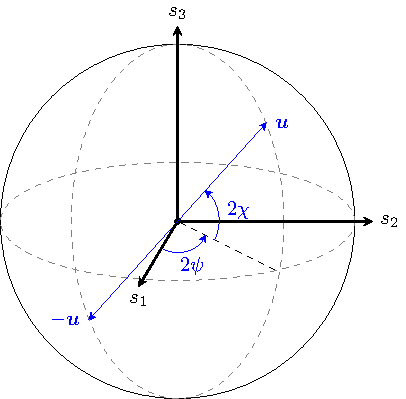
\includegraphics[scale=0.9]{images/theory/tikz_poincare_sphere_intro.pdf}
    \caption{Example of a normalized polarization state $\bm{u}$ on the surface of the Poincaré sphere and its associated orthogonal state $-\bm{u}$. All normalized fully polarized states exists on the surface of the sphere and the position of a specific normalized state is defined by the last three components of its corresponding Stokes vector.}
    \label{fig:poincare_sphere_intro}
\end{figure}

Several properties can be observed directly from this geometrical representation. For example all linear polarized states will exist in the plane with $s_3=0$. Similar, the points $s_{2+}(1,0,0)$, $s_{1-}(-1,0,0)$, $s_{2+}(0,1,0)$ and $s_{2-}(0,-1,0)$ are assigned to the linear polarization states whose planes of polarization are along the horizontal, vertical, \SI{+45}{\degree} and \SI{-45}{\degree} axes respectively. States with a positive ellipticity $\psi$ lie on the northern hemisphere and the RCP state is located at the north pole ($s_{3+}(0,0,1)$). Likewise, all points on the southern hemisphere correspond to states with a negative ellipticity and the point $s_{3-}(0,0,-1)$ at the south pole corresponds to the LCP state. Furthermore, a pair of points on opposing sides of the sphere correspond to a pair of orthogonal states. An example of this is shown in figure \ref{fig:poincare_sphere_intro} as the pair $\bm{u}$ and $-\bm{u}$. Another useful feature of this representation is that when the light propagates in a medium and the polarization state changes it describes a trajectory on the sphere. This makes it possible to visualize the effect of an optical element or even a series of elements on a given initial polarization state.

\subsection{Jones vectors}
\label{sec:jones_vectors}
The Jones vector is another commonly used representation of polarized light, which again like the Stokes representation has its own advantages and disadvantages. For example the phase information is conserved in the Jones representation but it can only describe fully polarized light. Unlike the Stokes parameters, the Jones vector is also able to account for interference effects. Another advantage of the Jones vector for calculations is that it is straight forward to obtain its components. Specifically, the Jones vector is given directly by the field components as:
\begin{equation}
    \label{eq:jones_vector1}
    \bm{\mathcal{E}} = 
    \begin{pmatrix}
    E_x(t) \\
    E_y(t)
    \end{pmatrix},
\end{equation}
where $E_x(t)$ and $E_y(t)$ are the scalar field components of the electric field. We assume propagation in the z-direction and therefore field components in the xy-plane. The Jones vectors actually forms a vector space unlike the Stokes vectors. In this notation it is possible to preserve the phase information of the wave, since it is not averaged out as for the Stokes parameters. If we assume a quasimonochromatic wave like it is given in equation \ref{eq:quasi_mono_efields} and define $u(t)=\Bar{k}z-\Bar{\omega}t$, then we can rewrite the Jones vector in complex form and factor out the phases:
\begin{equation}
    \label{eq:jones_vector2}
    \bm{\mathcal{E}} = e^{iu(t)}
    \begin{pmatrix}
    E_{0x(t)}e^{i\delta_x(t)} \\
    E_{0y(t)}e^{i\delta_y(t)}
    \end{pmatrix}.
\end{equation}
 Furthermore, if we consider the special case where the amplitudes and phases do not vary with time we get the time independent representation of the Jones vector:
 \begin{equation}
    \label{eq:jones_vector3}
    \bm{\mathcal{E}}=
    \begin{pmatrix}
    E_{0x}e^{i\delta_x} \\
    E_{0y}e^{i\delta_y}
    \end{pmatrix},
\end{equation}
where we have left out the global phase factor $e^{iu(t)}$, since it does not change the polarization state as we saw for example in section \ref{sec:polellipse}. The Jones vector is often normalized so that the sum of the squares of the components is equal to one. For example in the case of a field with $E_{0x}=E_{0y}$ and $\delta_x=\delta_y$ we get the normalized Jones vector:
\begin{equation}
    \bm{\mathcal{E}}_{\SI{45}{\degree}}= \frac{1}{\sqrt{2}}
    \begin{pmatrix}
    1 \\
    1
    \end{pmatrix},
\end{equation}
which is a \SI{45}{\degree} linear polarized state. A useful operation is the scalar or inner product of two Jones vectors $\bm{\tilde{u}}$ and $\bm{\tilde{v}}$ which is defined as:
\begin{equation}
    \bm{\tilde{u}}^{\dagger}\bm{\tilde{v}} = \left(u_1^{*}, u_2^{*} \right)
    \begin{pmatrix}
    v_1 \\
    v_2
    \end{pmatrix}
    = u_1^{*}v_1 + u_2^{*}v_2,
\end{equation}
where the superscript $\dagger$ denotes conjugate transpose. In the same sense as for real vectors two Jones vectors are therefore said to be orthogonal if their inner product is zero. Moreover, the inner product can be used to calculate the intensity of a polarization state as:
\begin{equation}
    I=|\bm{\mathcal{E}}|^2=\bm{\mathcal{E}}^{\dagger}\bm{\mathcal{E}}
\end{equation}

With this we can express any Jones vector in the polarization ellipse representation through the intensity $I$, the orientation angle $\psi$ and the ellipticity angle $\chi$ as follows:

\begin{align}
\begin{split}
    \bm{\mathcal{E}} &=
    \sqrt{I}
    \begin{pmatrix}
    \cos \chi \cos \psi - i\sin \chi \sin \psi \\
    \cos \chi \sin \psi + i\sin \chi \cos \psi
    \end{pmatrix}
    \\
    &=
    \sqrt{I}
    \begin{pmatrix}
    \cos \psi & -\sin \psi \\
    \sin \psi & \cos \psi
    \end{pmatrix}
    \begin{pmatrix}
    \cos \chi \\
    i\sin \chi
    \end{pmatrix},
\end{split}
\end{align}
where we see that the rightmost factor is a Jones vector representing elliptical polarized light. The matrix in the middle is simply a rotation matrix that rotates the Jones vector by the angle $\psi$ and the factor to the left is the overall amplitude. This direct correspondence between the polarization ellipse parameters and the Jones vectors shows us that they are able to fully describe any polarization state. Before we move on to the next section it is worth mentioning how the components of the Jones vector transform into other reference frames, since this will be useful in the description of rotated elements. So far the Jones vectors have been defined with respect to a pair of axes XY lying in the reference plane tangential to the wavefront. Evidently the Jones vector in this frame can be written as:
\begin{equation}
    \bm{\mathcal{E}} = E_x \bm{e}_x + E_y \bm{e}_y, \qquad 
    \bm{e}_x = 
    \begin{pmatrix}
    1 \\
    0
    \end{pmatrix},
    \;
    \bm{e}_y = 
    \begin{pmatrix}
    0 \\
    1
    \end{pmatrix},
\end{equation}
where the basis vectors $\bm{e}_x$ and $\bm{e}_y$ represents light linear polarized along the X and Y axes respectively. In fact any complex 2x1 vector can be regarded as a Jones vector. It is therefore clear that the Jones vectors form a vector space and with that other bases can be defined as well. Consequently, the reference frame change from XY to X'Y' can be represented by an orthogonal transformation which can be defined as:
\begin{equation}
    \label{eq:jones_vector_transformation}
    \bm{\mathcal{E}}' = \hat{Q}(\theta) \bm{\mathcal{E}}, \qquad
    \hat{Q}(\theta) =
    \begin{pmatrix}
    \cos \theta & \sin \theta \\
    -\sin \theta & \cos \theta
    \end{pmatrix},
\end{equation}
where $\hat{Q}(\theta)$ corresponds to a counterclockwise rotation about the Z axis by the angle $\theta$ as shown in figure \ref{fig:frame_rotation}. 

\begin{figure}[h]
    \centering
    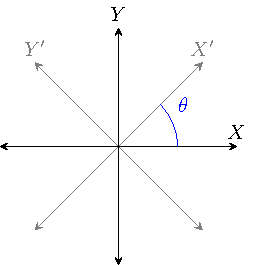
\includegraphics[scale=1]{images/theory/tikz_frame_rotation.pdf}
    \caption{An example of a coordinate transformation of the Jones vectors from the coordinate system with axes XY into the primed system. Such a transformation can be represented by a counterclockwise rotation by an angle $\theta$ around the Z axis.}
    \label{fig:frame_rotation}
\end{figure}

In the present chapter four different representations of the polarization state of a wave were introduced; the Poincaré sphere, the polarization ellipse, the Stokes and the Jones vectors, while the first two are useful for visualizing the state the latter two are practical for carrying out calculations. Specifically, certain calculations are better carried out using the Stokes parameters such as in the case of superimposing two incoherent light beams, while the Jones vector representation is better suited for describing fully polarized coherent light as in the context of this work. As an overview the normalized Stokes and Jones vectors of the degenerate polarization states are summarized in table \ref{tab:pol_statevectors}. Nonetheless, the degrees of polarization are readily obtained using the Stokes parameters, which are useful since they give a measure of the distance between a given polarization state and the degenerate polarization states. We further discussed how the polarization dependent interface transmission, dichroism and birefringence all affect the polarization state to different degrees. Additionally, we saw that a stratified structure can give rise to a special type of birefringence called form birefringence. As mentioned earlier both sets of vectors have a set of matrices associated with them, where the Jones matrices are a subset of the Mueller matrices. However, we will limit the following description to the Jones calculus, since in the context of this work it provides a sufficient mathematical framework for describing the polarization and changes of the polarization state caused by nondepolarizing media. How these matrices relate to optical elements and especially waveplates will be shown in the following chapter.

%TODO_2 section above (done)

\begin{table}[H]
    \centering
    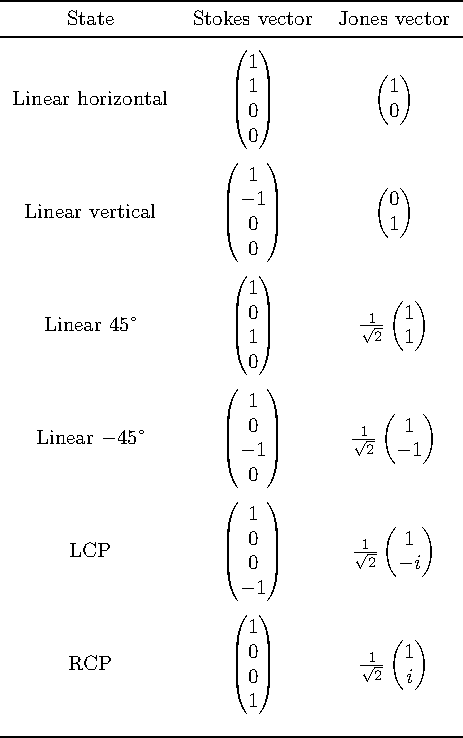
\includegraphics[scale=1]{images/theory/pol_statevectors_table.pdf}
    \caption{Summary of all the normalized Jones and Stokes vectors for the degenerate polarization states.}
    \label{tab:pol_statevectors}
\end{table}

% TODO1 add remark that we first consider some general useful properties or features of jones matrices and then look at the individual implementations representing different optical elements (Done)

% TODO2 section title :) (or Mathematical description of nondepolarizing media or mathematical calculus or something) (Done)

% TODO note form birefringence allows avoiding stacking and almost arbitrary number of plates limited by cpu power (goes as n squared) ?

% TODO maybe define bandwidth like masson?

% TODO remove r, use j00, j10 instead. (done)

% Describe a little more how we get J... and parameters a,b,d,psi,mu (done)

% TODO add remark that retardation is delay between eigenstates or equivalently the difference of the two eigenvalue phases (done?)

% TODO check T_1/4. yea that part's fuckd (done?? check again)

% TODO Masson polar decomp and compare to elliptical with A,B.. matrix. Check what I wrote.

% TODO for results?. Give explanation why two l4 dont give l2. Problem is l4 is also rotator (is it?) -> different azimuths -> different outputs since l4 is rotator depending on azimuth ... (done)

% only for 100% pure circ is azimuth undef. (never happens)

% TODO write summary + transition to chapter 4, right? depends on final structure

% TODO remark that passivity means that abs(T_ij) <= 1 used in l_2 loss function.


\chapter{Waveplate design}
\label{ch:wp_design}
The composite AWP proposed in this work consists of a number of birefringent waveplates stacked at different azimuths relative to the optical axis. The set of characteristic dimensions of the waveplates together with the azimuthal angles therefore define a specific design. The characteristic dimensions of a waveplate are its thickness and stratification dimensions. In the first section of this chapter we give a phenomenological introduction to waveplates and following we present the Jones calculus which can be used to describe the polarization change of any non-depolarizing media such as birefringent waveplates. Subsequently we introduce and categorize waveplates in the context of the Jones calculus. The procedure of obtaining a design mainly consists of optimizing an objective function which is in turn based on the Jones calculus, which is described in the final section of this chapter.

\section{Waveplates}
\label{sec:waveplates}
To explain how a waveplate works we assume that the materials are non-absorbing and neglect interface effects. Additionally, to avoid refraction we always assume normal incidence of the light beam on the waveplate. In the case where we only consider birefringence the operation of a waveplate or retarder is fairly simple. One of the two polarization states of the wave is caused to have its phase evolve faster compared to the other state. Therefore, depending on the distance the wave travels in the waveplate, the amount one field component is lagging behind the other can be controlled. Using this principle it is in theory possible to convert any initial polarization state into any other state. This is shown in figure \ref{fig:waveplate_conversions}, where the positive values indicate that $E_y$ leads $E_x$ and similarly the negative values show that $E_y$ lags behind $E_x$ by the indicated amount. The waveplates in the context of this work consists of uniaxial materials i.e. they have a single optic axis. Therefore, if the $E_y$ component aligns with the fast axis, which is the axis with the lowest refractive index of the waveplate, then it is advanced compared to the $E_x$ component. Likewise, if the $E_y$ component is aligned with the slow axis of the waveplate then the $E_x$ component is advanced. Similarly, the slow axis is the axis or direction with the highest refractive index. The phase difference between two adjacent states in figure \ref{fig:waveplate_conversions} is $\frac{\pi}{4}$. Going clockwise this phase shift is subtracted and vice versa in the counterclockwise direction, so that eight steps make a full cycle. For example, if linearly polarized light is sent through a waveplate with its fast axis along the y-axis then the state will be shifted counterclockwise using the convention that $\delta=\delta_y-\delta_x$. This means that a phase shift of $-\frac{\pi}{2}$ causes \SI{45}{\degree} linear polarized light to emerge LCP and RCP for a phase shift of $+\frac{\pi}{2}$. Likewise, a phase shift of $\pm \pi$ causes the light to remain linearly polarized but with its plane of polarization rotated by \SI{90}{\degree}.

\begin{figure}[h]
    \centering
    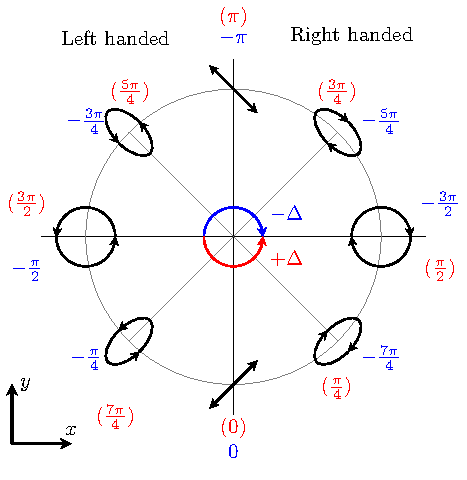
\includegraphics[scale=1.3]{images/theory/tikz_waveplate_conversions.pdf}
    \caption{The different polarization states when the y-component leads or lags behind the x-component by the indicated phase shifts $\pm \Delta$. Each step in the counterclockwise or clockwise direction subtracts or adds a phase shift of $\frac{\pi}{4}$, respectively.}
    \label{fig:waveplate_conversions}
\end{figure}

If we assume that the incident wave has components parallel and perpendicular to the optic axis of the waveplate, then two separate waves will propagate in the waveplate as we have seen in the previous chapter, that is the e- and o-wave. The phase speed of the e-wave is higher than that of the o-wave. Furthermore, if the incident light is parallel or perpendicular to the optic axis as in this case then we see no refraction of either of the waves, the final emerging wave will therefore be a superposition of the e- and o-wave. Additionally, due to the different phase velocities, the two waves will have a phase difference of $\Delta$ after passing through the waveplate. This phase difference is known as the retardance of the waveplate. For a waveplate of thickness $d$ the optical path difference is then given by:
\begin{equation}
    \Lambda = d|n_o - n_e|
\end{equation}
with $\Delta = k_0 \Lambda$ we therefore get the following expression for the phase difference:
\begin{equation}
    \label{eq:wp_eq}
    \Delta = \frac{2\pi}{\lambda_0}d|n_o - n_e|,
\end{equation}
where $\lambda_0$ is the wavelength of the wave in free space. There are three special types of waveplates: full, half and quarter waveplates. The full waveplate causes a phase shift of $2\pi$. That means the retardation is one wavelength or a full cycle in figure \ref{fig:waveplate_conversions}. The initial polarization state is therefore not altered. It is important to emphasize that this is only the case for monochromatic light. Since the materials in general are dispersive and because $\Delta$ directly varies as $\lambda_0^{-1}$. The condition that $\Delta = 2\pi$ or any other value can therefore only be fulfilled for monochromatic waves. This means in general that waveplates are chromatic which is the main problem with which we are concerned in this work. Full waveplates can therefore be used as narrow-wavelength filters if they are placed in between two crossed polarizers. Only the frequency component for which $\Delta$ is $2\pi$ will not have a component parallel to the final polarizer. 

A half waveplate causes a phase shift of $\pi$ between the e- and o-wave. Furthermore, we assume in the following that the initial polarization is linear and the plane of polarization is at some angle $\theta$ relative to the fast axis of the waveplate. As the name suggests, this phase shift causes one component to be delayed by half a wavelength relative to the other component. In the case of a positive uniaxial material this means that the e-wave is delayed by half a wave and the plane of polarization will be rotated by $2\theta$. An example of a half waveplate is shown in figure \ref{fig:half_waveplate}. In this example the material of the waveplate is positive uniaxial. Since then $n_o<n_e$ so that the e-wave is delayed relative to the o-wave. For a given wavelength and material it follows from equation \ref{eq:wp_eq} that $d$ must be equal to $\frac{1}{2}\frac{\lambda_0}{|n_o - n_e|}$. 

\begin{figure}[h]
    \centering
    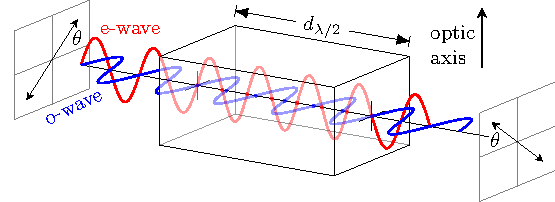
\includegraphics[scale=1.45]{images/theory/tikz_half_waveplate.pdf}
    \caption{A half waveplate consisting of a positive uniaxial material. The e-wave is delayed relative to the o-wave since it propagates slower. Adjusting the thickness $d_{\lambda/2}$ gives a final relative phase shift of $\pi$. This phase shift causes the polarization plane to be rotated by $2\theta$, where $\theta$ is the angle between the fast axis and the polarization plane of the waveplate. The dots along the axis of propagation indicate half a wavelength of the similar colored wave.}
    \label{fig:half_waveplate}
\end{figure}

As we saw earlier in figure \ref{fig:waveplate_conversions}, the polarization state is periodic with a periodicity of $2\pi$. It therefore follows from equation \ref{eq:wp_eq} that a waveplate with an additional thickness of $d_{\lambda}=\frac{\lambda_0}{|n_o - n_e|}$ still functions as a half waveplate. And with the same reasoning, an additional thickness of $md_{\lambda}$ (where $m$ is a whole number) does not change the final polarization state. The thickness of a half waveplate is therefore given by:

\begin{equation}
    \label{eq:thickness_half_waveplate}
    d_{\lambda/2} = \frac{(2m+1)\lambda_0}{2|n_o - n_e|}, \quad m=0,1,2,... 
\end{equation}

Furthermore, the effect that a half waveplate rotates the plane of polarization by $2\theta$ is also true for other elliptical polarization states. This is because a half waveplate always shifts one component by half a wave relative to the other component. Additionally, the handedness of the polarization state is inverted. We see this from figure \ref{fig:waveplate_conversions} where the effect of a half waveplate corresponds to half a rotation in the diagram. In other words, the final state is always on the opposite side of the initial state in the diagram. It is worth noting at this point, that linearly polarized light for which the polarization plane aligns with the slow or fast axis of any waveplate is unaffected by a waveplate, since in that case the light only has one component.

The final of the three special waveplate types is the quarter waveplate. Again, as the name suggests it shifts the relative phase by a quarter period or $\frac{\pi}{2}$. For linearly polarized light at an angle of \SI{45}{\degree} to either the slow or fast axis of a quarter waveplate, the light is converted into circular polarized light. An example of this setting is shown in figure \ref{fig:quarter_waveplate}.

\begin{figure}[H]
    \centering
    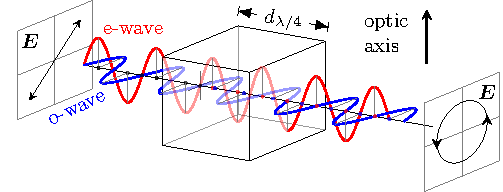
\includegraphics[scale=1.55]{images/theory/tikz_quarter_waveplate.pdf}
    \caption{\SI{45}{\degree} Linearly polarized light incident on a quarter waveplate consisting of a positive uniaxial material. In this case the slow axis is therefore along the optic axis. The thickness $d_{\lambda/4}$ is chosen so that the final phase difference between the e-wave and the o-wave is $\pi/2$. The final state is LCP since the material is positive uniaxial, for a negative uniaxial material it would be RCP. The colored dots indicate the accumulated phase difference.}
    \label{fig:quarter_waveplate}
\end{figure}

Because of the fact that the amplitudes of the components along the fast and slow axis initially are equal it follows that the final polarization state is circular. The same reasoning can be applied to circular light, which a quarter waveplate converts into linearly polarized light. Again, figure \ref{fig:waveplate_conversions} also gives an overview of some of the different possible conversions caused by a quarter waveplate. Specifically, a quarter waveplate shifts the polarization state a quarter cycle in the diagram. Similar to a half waveplate we get that the thickness $d_{\lambda/4}$ of a quarter waveplate is given by:

\begin{equation}
    \label{eq:thickness_quarter_waveplate}
    d_{\lambda/4} = \frac{(4m+1)\lambda_0}{4|n_o - n_e|}, \quad m=0,1,2,... 
\end{equation}

The number $m$ is known as the order of the waveplate. An order of $0$ means that it is the thinnest possible realization of a specific waveplate type. These waveplates are referred to as zero-order waveplates. Likewise, multiple-order waveplates have thicknesses that are a multiple of a full $2\pi$ phase shift plus the type specific phase shift. Evidently, for multiple-order waveplates $m$ is larger than zero. Waveplates are often multiple-order. For example a quartz quarter waveplate with a birefringence of $0.0092$ would have a thickness of only \SI{15}{\micro \meter} for a wavelength of \SI{550}{\nano \meter}. This makes it fragile as well as difficult to produce in contrast to a thicker multiple-order quarter waveplate. The two waveplates shown in figure \ref{fig:half_waveplate} and \ref{fig:quarter_waveplate} are examples of zero-order waveplates. The frequencies with which we are concerned in this work are in the higher GHz and the lower THz range. Consequently, already a zero-order quarter or half waveplate designed for these frequencies will have a thickness in the lower millimeter or centimeter range. A part of the problem is therefore to reduce the order of the designed waveplates, i.e. to keep them as thin as possible. This has to be taken into consideration since for higher orders the waveplates quickly become fairly thick which makes them impractical mainly due to high absorption losses \cite{Hecht}.

It is clear that it would quickly become complicated to predict the final polarization state of a polarized wave, after it has passed a series of waveplates and polarizers. Especially the way we have done it so far by considering polarization in terms of the individual field components. In the following section we will therefore introduce a better suited alternative method of describing the polarization and changes thereof. We will see that any polarization state can be described by a vector and each optical element by a matrix. This method reduces most calculations to matrix multiplications, which is especially useful for solving problems consisting of a series of optical elements.

\section{Jones calculus}
\label{sec:jonescalc}
The Jones calculus or specifically the Jones matrices can be used to describe the non-depolarizing polarimetric interaction of fully polarized light with matter. For that we first introduce a few general properties of the Jones matrices. In the following section we will then apply these properties to describe and categorize the different types of waveplates. Evidently, the following description of optical elements is only valid for changes with a linear relationship between the input and output amplitudes since it is based on a system of linear equations. Under these assumptions we can then express any transformation of an initial or input polarization state $\bm{\mathcal{E}}$ into another final output state $\bm{\mathcal{E}}'$ as:
\begin{equation}
    \bm{\mathcal{E}}' = \hat{T} \bm{\mathcal{E}},
\end{equation}
where $\hat{T}$ is the 2x2 complex Jones matrix specifying the interaction. With this many of the common operations defined in linear algebra can be reused and given a physical interpretation in the Jones calculus. For example the matrix product of two Jones matrices $\hat{T}_1$ and $\hat{T}_2$ represents a so called series or train of optical elements, where each matrix describes the polarimetric change caused by the respective element. This can be extended to multiple elements so that the final state in a train of $n$ consecutive elements is given by:
\begin{equation}
    \label{eq:jones_series_product}
    \bm{\mathcal{E}}' = \prod_{i=1}^{n} \hat{T}_i \bm{\mathcal{E}}.
\end{equation}
It is clear that since the product of two matrices does in general not commute the order of the factors is important \cite{Jones1941}. Therefore if $\hat{T}_1$ is the first element encountered by the light then the order of the indices has to be reversed. It is worth noting that in general the action of materials on the input state depends on the properties of the wave as well as how the interaction takes place. For example reflection from a surface depends on the incident angle or in case of waveplates the phase shift is proportional to the frequency. The Jones matrices themselves can therefore depend on a number of parameters reflecting the properties of the interaction, material and input state. Furthermore, since all Jones matrices are 2x2 complex matrices they can be factored into a product of three matrices using the singular value decomposition. This means we can express any Jones matrix $\hat{T}$ in the following form:
\begin{equation}
    \label{eq:jones_singular_value_decomposition}
    \hat{T} = \hat{T}_{R2}\diag{p_1, p_2}\hat{T}_{R1},
\end{equation}
where $\hat{T}_{R1}$ and $\hat{T}_{R2}$ are unitary\footnote{A complex square matrix $\hat{U}$ is unitary if $\hat{U} \hat{U}^\dagger=\hat{I}$ where $\hat{I}$ is the identity matrix} matrices and $\diag{p_1, p_2}$ is a diagonal matrix whose entries are the singular values of $\hat{T}$. The squares of $p_1$ and $p_2$ can be calculated directly using the following expressions:
\begin{equation}
    p_{1,2}^2 = \frac{1}{2}\left(\tr(\hat{T}\hat{T}^{\dagger}) \pm 
    \sqrt{\tr(\hat{T}\hat{T}^{\dagger})^2-4\det(\hat{T}\hat{T}^{\dagger})}\right),
\end{equation}
where $\tr$ is the matrix trace and the sign is positive and negative for $p_1$ and $p_2$, respectively. The physical interpretation of these two values becomes evident if we consider the effect of the matrix $\diag{p_1, p_2}$ on an input state. Specifically, it simply scales the amplitudes of the state and with that also the intensity. Additionally, since the singular values are non-negative and real we can assume that $p_2\leq p_1$. Therefore, if the light is not amplified by the element in question then we get the following condition:
\begin{equation}
    \label{eq:passitivity_condition}
    p_1^2 \leq 1,
\end{equation}
which is also a defining property of Jones matrices. In other words a complex 2x2 matrix is a Jones matrix if equation \ref{eq:passitivity_condition} is satisfied \cite{Barakat1987}. Similar to Jones vectors the Jones matrices are defined up to an arbitrary phase factor $e^{i\phi}$, which means that two matrices $\hat{T}$ and $e^{i\phi}\hat{T}$ are equivalent in the sense that their respective final output states have equal intensities. A standard convention is therefore to assume that $\det \hat{T}$ is positive. Furthermore, the representation of a Jones matrix in another coordinate system follows directly from the coordinate transformation for Jones vectors given by equation \ref{eq:jones_vector_transformation}. Specifically, the transformation of a Jones matrix $\hat{T}$ in system XY to another representation $\hat{T}'$ in system X'Y' is given by:
\begin{equation}
    \label{eq:jones_matrix_transformation}
    \hat{T}' = \hat{Q}(\theta)\hat{T}\hat{Q}(-\theta).
\end{equation}
It is important to distinguish between frame rotations and rotations of the actual element. In the first case we rotate the axes and the second case can be understood as a rotation of the vector. Therefore, in the case of a rotation of the element around the Z-axis the signs of the rotation matrices in equation \ref{eq:jones_matrix_transformation} are inverted. It is worth noting that we only have to consider rotations since they are the only geometrical transformations that actually preserve the physically invariant quantities \cite{GilPerez2017}. Another interesting concept are singular states of polarization. Specifically, the singular value decomposition readily shows that for any Jones matrix there exists two pairwise orthonormal states $\tilde{\bm{\eta}}_1$ and $\tilde{\bm{\eta}}_2$ for which the orthogonality is preserved, in other words their respective output states $\bm{\eta}_1'$ and $\bm{\eta}_2'$ are mutually orthogonal. Furthermore, from the definition of the singular values the states $\tilde{\bm{\eta}}_1$ and $\tilde{\bm{\eta}}_2$ are orthonormal eigenvectors of the matrix $\sqrt{\hat{T}\hat{T}^{\dagger}}=\hat{T}_{R1}^{\dagger}\diag{p_1, p_2}\hat{T}_{R1}$ and are given explicitly by the columns of $\hat{T}^{\dagger}$. We can therefore express the singular states as:
\begin{equation}
    \bm{\eta}_1 = \hat{T}^{\dagger}_{R1}\begin{pmatrix} 1 \\ 0 \end{pmatrix}, \qquad
    \bm{\eta}_2 = \hat{T}^{\dagger}_{R1}\begin{pmatrix} 0 \\ 1 \end{pmatrix},
\end{equation}
and calculate the output states:
\begin{align}
\begin{split}
    \bm{\eta}'_1 &= \hat{T}\tilde{\bm{\eta}}_1 = 
    p_1\hat{T}_{R2}\hat{T}_{R1}\tilde{\bm{\eta}}_1 =
    p_1\hat{T}_{R2}\begin{pmatrix} 1 \\ 0 \end{pmatrix}, \\
    \bm{\eta}'_2 &= \hat{T}\tilde{\bm{\eta}}_2 = 
    p_2\hat{T}_{R2}\hat{T}_{R1}\tilde{\bm{\eta}}_2 =
    p_2\hat{T}_{R2}\begin{pmatrix} 0 \\ 1 \end{pmatrix}.
\end{split}
\end{align}
These expressions for the final states can then be used to calculate their respective intensities as:
\begin{equation}
    \bm{\eta}'^{\dagger}_1\bm{\eta}'_1=p_1^2, \qquad 
    \bm{\eta}'^{\dagger}_2\bm{\eta}'_2=p_2^2, \qquad 
    \bm{\eta}'^{\dagger}_1\bm{\eta}'_2=0.
\end{equation}
If we further define the transmittance as the ratio between the transmitted intensity and the incident intensity, then we see that the states $\bm{\eta}_1$ and $\bm{\eta}_2$ are exactly the states with the highest and lowest transmittance, respectively. In other words, with respect to any other normalized output state, the states $\bm{\eta}'_1$ and $\bm{\eta}'_2$ are the output states with the highest and lowest intensities, respectively. The last property we will introduce before applying these to describe waveplates in the Jones calculus is the normality of Jones matrices. As we shall see later this property is important for the calculation of the retardance for a given Jones matrix. Additionally, Jones matrices can be separated into two categories depending on the mutual orthogonality of their eigenvectors $\bm{\mathcal{E}}_q$ and $\bm{\mathcal{E}}_r$. The eigenvectors which are also known as the eigenstates or eigenpolarizations of $\hat{T}$ can be interpreted by considering their defining equations:
\begin{equation}
    \hat{T}\bm{\mathcal{E}}_q = \lambda_q\bm{\mathcal{E}}_q, \qquad 
    \hat{T}\bm{\mathcal{E}}_r = \lambda_r\bm{\mathcal{E}}_r,
\end{equation}
where $\lambda_q = |\lambda_q|e^{i\delta_q}$ and $\lambda_r = |\lambda_r|e^{i\delta_r}$ are the associated complex eigenvalues. In other words, the application of $\hat{T}$ to the eigenstates only scales them by a complex number but leaves the polarization type unchanged. Hence if $\bm{\mathcal{E}}_q$ and $\bm{\mathcal{E}}_r$ are mutually orthogonal then the Jones matrix is said to be normal or homogeneous and nonnormal or inhomogeneous if they are nonorthogonal. We can therefore define the nonnormality or inhomogeneity parameter $\eta$ as follows:
\begin{equation}
    \eta=|\bm{\mathcal{E}}^{\dagger}_q \bm{\mathcal{E}}_r|.
\end{equation}
This means that the inhomogenity is zero if $\hat{T}$ is normal and one if the eigenvectors are parallel, where the latter is also known as the degenerate case. To calculate the inhomogeneity and verify that a given Jones matrix $\hat{T}$ is normal we use another derived expression for $\eta^2$ which is given by:
\begin{equation}
    \eta^2 = \frac{2||\hat{T}||_2^2-|\tr\hat{T}|^2-|(\tr\hat{T})^2-4\det\hat{T}|}{2||\hat{T}||_2^2-|\tr\hat{T}|^2+|(\tr\hat{T})^2-4\det\hat{T}|},
\end{equation}
where $||\hat{T}||_2=\sqrt{\tr \hat{T}^{\dagger} \hat{T}}$ denotes the Frobenius norm of $\hat{T}$ \cite{Lu1994}. With this we can introduce and categorize waveplates in the context of the Jones calculus which is shown in the following section. 

\section{Waveplates and Jones calculus}
\label{sec:jones_calc}
% TODO_2 this section below
In the first section of this chapter we presented a phenomenological description of waveplates for which we assumed them to be fully transparent, i.e. the intensity of the incident light was equal to the intensity of the transmitted light. Under this assumption such ideal elements only exhibit birefringence and we will therefore refer to them as retarders or ideal waveplates. Furthermore, in the Jones calculus these ideal waveplates are represented by unitary matrices. Later in this section we will describe and add diattenuators to the framework. The diattenuator will allow us to quantify absorption by the waveplates and it especially simplifies the description of anisotropic absorption effects such as dichroism, reflection losses and transmission losses. In theory combined the retarder and diattenuator, known as a diattenuating retarder, constitute a complete model of the waveplate and even of any non-depolarizing material. In the following we classify and categorize retarders according to the polarization type of their eigenstates, consequently there are three different types of retarders; elliptic, circular and linear. 

\subsection{Retarders}
Similar to the different polarization types the most general type of retarder is the elliptic retarder which is characterized by the following eigenstates:
\begin{align}
\begin{split}
    \label{eq:ellip_pol_eigenstates}
    \bm{\mathcal{E}}_1(\alpha, \delta) &= 
    \begin{pmatrix} c_{\alpha} e^{-i\delta /2} \\ s_{\alpha} e^{i\delta /2} \end{pmatrix}
    = 
    \begin{pmatrix} c_{\chi} c_{\psi} - i s_{\chi} s_{\psi} \\ 
    c_{\chi} s_{\psi} + i s_{\chi} c_{\psi} \end{pmatrix},
    \\
    \bm{\mathcal{E}}_2 \left( \frac{\pi}{2} - \alpha, \delta+\pi \right) &= 
    \begin{pmatrix} -i s_{\alpha} e^{-i\delta /2} \\ i c_{\alpha} e^{i\delta /2} \end{pmatrix}
    = 
    \begin{pmatrix} -c_{\chi} s_{\psi} + i s_{\chi} c_{\psi} \\ 
    c_{\chi} c_{\psi} + i s_{\chi} s_{\psi} \end{pmatrix},
\end{split}
\end{align}
where we have set $\sin(x) = s_x$ and $\cos(x) = c_x$ which we use from here on. We see that $\bm{\mathcal{E}}_1$ and $\bm{\mathcal{E}}_2$ are both general elliptical polarization states, where the specific shape of their respective polarization ellipses is determined by the parameters $\alpha$ and $\delta$. It is worth emphasizing that $\delta$ is not the phase difference of the input state but a characterizing parameter of the retarder also known as the circularity. The corresponding Jones matrix $T_R(\alpha, \delta, \Delta)$ representing the elliptical retarder is given by:
\begin{equation}
    \hat{T}_R(\alpha, \delta, \Delta) = 
    \begin{pmatrix} 
    c^2_{\alpha}  e^{i\Delta /2} + s^2_{\alpha} e^{-i\Delta /2} & i s_{2\alpha} s_{\Delta/2} e^{-\delta} \\ 
    i s_{2\alpha} s_{\Delta/2} e^{-\delta} & s^2_{\alpha} e^{i\Delta/2} + c^2_{\alpha} e^{-i\Delta /2}
    \end{pmatrix}, 
\end{equation}
which introduces a phase difference of $\Delta$ between its eigenstates $\bm{\mathcal{E}}_1$ and $\bm{\mathcal{E}}_2$. In other words we can define the retardance $\Delta$ in terms of the arguments or phases of the eigenvalues as follows:
\begin{equation}
    \label{eq:jones_ret_def}
    \Delta = |\delta_r-\delta_q|.
\end{equation}
This is a reasonable definition if we consider the definition of the eigenstates and the polar form of the eigenvalues. That is the global phase change, which is also the only change, of each eigenstate is the phase of the eigenvalue. Especially, in the case of birefringent waveplates for which the linear eigenstates align with the fast and slow axis of the birefringent material we get exactly an additional phase shift of $\Delta$ between field components along said axes. Furthermore, we see that this is in fact the most general representation of a retarder, since the coefficients of any 2x2 unitary matrix can be factorized in this manner. If we change the frame in which we represent $\hat{T}_R(\alpha, \delta, \Delta)$ so that it aligns with the mayor and minor axes of the polarization ellipse of $\bm{\mathcal{E}}_1$, then $\psi=0$ for an orientation of \SI{0}{\degree} and therefore $\delta=\frac{\pi}{2}$, $\alpha=\chi$. With this the Jones matrix reduces to the following:
\begin{equation}
    \hat{T}_R\left(\chi, \frac{\pi}{2}, \Delta\right) = 
    \begin{pmatrix} 
    c^2_{\chi} e^{i\Delta /2} + s^2_{\chi} e^{-i\Delta /2} & s_{2\chi} s_{\Delta/2} \\
    -s_{2\chi} s_{\Delta/2} & s^2_{\chi} e^{i\Delta /2} + c^2_{\chi} e^{-i\Delta /2}
    \end{pmatrix}. 
\end{equation}

In the case of circular polarized eigenstates $\bm{\mathcal{E}}_1$ and $\bm{\mathcal{E}}_2$ the polarization ellipse reduces to a circle and $\chi=\frac{\pi}{4}$ so that $\delta=\frac{\pi}{2}$ and $\alpha=\frac{\pi}{4}$. A retarder with circular eigenstates is known as a circular retarder or rotator since in this case the Jones matrix takes on the following form:
\begin{equation}
    \hat{T}_{RC}(\Delta)=\hat{T}_R\left(\frac{\pi}{4}, \frac{\pi}{2}, \Delta\right) = 
    \begin{pmatrix} 
    c_{\Delta/2} & s_{\Delta/2} \\
    -s_{\Delta/2} & c_{\Delta/2}
    \end{pmatrix},
\end{equation}
which is also the representation of a rotation matrix $\hat{Q}(\theta)$ with $\theta=\Delta/2$. In other words the effect of $\hat{T}_{RC}(\Delta)$ is equal to a rotation of the principal axes of an incident state by $\theta=\Delta/2$. The final type is the linear retarder which is characterized by having linear eigenstates. For this type $\chi=0$, therefore $\delta=0$ and $\alpha=\psi$. With this the Jones matrix of the linear retarder is given by:
\begin{equation}
    \hat{T}_{RL}\left(\psi, \Delta\right) = 
    \begin{pmatrix} 
    c^2_{\psi} e^{i\Delta /2} + s^2_{\psi} e^{-i\Delta /2} & is_{2\psi} s_{\Delta/2} \\
    is_{2\psi} s_{\Delta/2} & s^2_{\psi} e^{i\Delta /2} + c^2_{\psi} e^{-i\Delta /2}
    \end{pmatrix},
\end{equation}
and if we again align the coordinate frame with the mayor and minor axes of its eigenstates then $\psi=0$ and $\hat{T}_{RL}$ adopts the following diagonal form:
\begin{equation}
    \hat{T}_{RL}\left(\psi=0, \Delta\right) \equiv \hat{T}_{RL0}\left(\Delta\right) = 
    \begin{pmatrix} 
    e^{i\Delta /2} & 0 \\
    0 & e^{-i\Delta /2}
    \end{pmatrix},
\end{equation}
which is known as a horizontal linear retarder. In this frame we directly recognize the total phase shift $\Delta$ of the eigenstates. Furthermore, we see that the mayor and minor axis of the polarization ellipse of the eigenstates align with the fast and slow axis of the retarder. If we set $\Delta=\pi$ in the expression for the linear retarder we get the Jones matrix for the half wave retarder or transparent half waveplate as follows:
\begin{equation}
    \hat{T}_{RL}(\psi, \pi)= 
    \begin{pmatrix} 
    c_{2\psi} & s_{2\psi} \\
    s_{2\psi} & -c_{2\psi}
    \end{pmatrix}.
\end{equation}
We see that $\hat{T}_{RL}(\psi, \pi)$ is equivalent to a rotation by $-2\psi$ and an inversion of the y-component where the latter can be represented by $\hat{T}_{RL}(0, \pi)$. Therefore, essentially $\hat{T}_{RL}(\psi, \pi)$ inverts the handedness and then rotates the polarization ellipse of the state by $-2\psi$. These two actions combined are also known as an improper rotation. A circular polarized state therefore remains circular but has its handedness reversed by the action of $\hat{T}_{RL}(\psi, \pi)$. Finally, we can also see this by writing $\hat{T}_{RL}(\psi, \pi)$ to obtain the following representation of the Jones matrix describing the half wave retarder:
\begin{equation}
    \label{eq:l2_wp_effect}
    \hat{T}_{RL}(\psi, \pi)\equiv
    \hat{T}_{1/2}(\psi)=
    \hat{Q}(-2\psi)\hat{T}_{RL}(0, \pi)=\hat{Q}(-2\psi)\diag{1,-1}.
\end{equation}
If the input light is for example linear horizontal polarized and $\psi=\frac{\pi}{4}$ then the inversion leaves the state unaffected but the rotation produces an output state which is linear vertical polarized.
Similarly, if we set $\Delta=\pi/2$ then the expression for the linear retarder reduces to the following:
\begin{align}
\begin{split}
    \hat{T}_{1/4}(\psi)\equiv\hat{T}_{RL}(\psi, \pi/2)
    &=\frac{1}{\sqrt{2}}\left(\hat{I}+i\hat{Q}(-2\psi)\hat{T}_{RL}(\pi, \pi)\right)
    \\
    &=\frac{1}{\sqrt{2}}\left(\hat{I}+i\hat{T}_{1/2}(\psi)\right),
\end{split}
\end{align}
which is the Jones matrix for a quarter wave retarder. This expression shows that $\hat{T}_{RL}(\psi, \pi/2)$ is equivalent to the effect of $\hat{T}_{1/2}(\psi)$ followed by a \SI{90}{\degree} phase shift this new state is then superimposed on the input state. For example a linear horizontal state is first transformed into a linear vertical polarized state and then shifted by a quarter period. This rotated and shifted state is then further superimposed on the horizontal input state so that the output state will be RCP. 

It is in fact possible to represent any linear retarder using a combination of rotation matrices $\hat{Q}$ and horizontal linear retarders $\hat{T}_{RL0}$ as follows:
\begin{equation}
    \hat{T}_{RL}(\psi, \Delta)=\hat{T}_{RC}(-2\psi)\hat{T}_{RL0}(\Delta)\hat{T}_{RC}(2\psi)=
    \hat{Q}(-\psi)\hat{T}_{RL0}(\Delta)\hat{Q}(\psi).
\end{equation}
In other words a linear retarder is equivalent to a horizontal linear retarder $\hat{T}_{RL0}(\Delta)$ placed between a left- and right-handed circular retarder $\hat{T}_{RC}(-2\psi)$ and $\hat{T}_{RC}(2\psi)$, respectively. In general an elliptic retarder $\hat{T}_R(\alpha, \delta, \Delta)$ can be realized by the following combination of elements \cite{GilPerez2017}:
\begin{equation}
    \hat{T}_R(\alpha, \delta, \Delta)=
    \hat{T}_{RL0}(-\delta)\hat{Q}(-\alpha)\hat{T}_{RL0}(\Delta)\hat{Q}(\alpha)\hat{T}_{RL0}(\delta).
\end{equation}

\subsection{Diattenuators}
In the following we will introduce the diattenuator in a similar fashion as we did with the retarder. It is used to describe the polarization dependent transmittance of the waveplate. Any element for which the singular values $p_1$ and $p_2$ of its Jones matrix are mutually different can be considered a diattenuator \cite{Savenkov2005}. This means that for example matrices $\hat{T}_r$ and $\hat{T}_t$ describing the transmission and reflection at an interface are examples of Jones matrices representing diattenuators. If we further consider homogeneous diattenuators then we can again use a singular value decomposition as in equation \ref{eq:jones_singular_value_decomposition} to factorize the diattenuator Jones matrix as follows:
\begin{equation}
    \label{eq:diattenuator_singular_value_decomposition}
    \hat{T}_D = \hat{T}_D^{\dagger} = \hat{T}_R\hat{T}_{DL0}\hat{T}_R^{\dagger}, 
    \qquad 
    \hat{T}_{DL0}=\diag{p_1, p_2}.
\end{equation}
We know from the previous section that $p_1^2$ and $p_2^2$ are the maximum and minimum transmittance, respectively. We can therefore use $p_1$ and $p_2$ to define the diattenuation in the Jones calculus as follows: 
\begin{equation}
    \label{eq:diattenuation_1}
    D = \frac{p_1^2-p_2^2}{p_1^2+p_2^2}
\end{equation}
Furthermore, as with the retarders the diattenuators are also grouped or categorized based on the polarization type of their associated eigenstates. This means that the most general type of homogeneous diattenuators is the elliptic diattenuator with eigenstates given in equation \ref{eq:ellip_pol_eigenstates}. Additionally, equation \ref{eq:diattenuator_singular_value_decomposition} shows that the diattenuator is represented by a Hermitian\footnote{A complex square matrix $\hat{H}$ is Hermitian if $\hat{H}=\hat{H}^{\dagger}$.} matrix. This means that the Jones matrix of the most common or general diattenuator can be written as:
\begin{equation}
    \hat{T}_D(\alpha, \delta, p_1, p_2) = 
    \begin{pmatrix} 
    p_1 c_{\alpha}^2 + p_2 s_{\alpha}^2 & s_{\alpha}c_{\alpha}(p_1-p_2)e^{-i\delta} \\
    s_{\alpha}c_{\alpha}(p_1-p_2)e^{i\delta} & p_1 s_{\alpha}^2 + p_2 c_{\alpha}^2
    \end{pmatrix},
\end{equation}
for which we assume that $0\leq p_2\leq p_1$. If $p_2=0$ then $\hat{T}_D(\alpha, \delta, p_1, 0)$ represents a total elliptic polarizer which completely absorbs the $\bm{\mathcal{E}}_2$ eigenstate. If we align the axes of the frame in which $\hat{T}_D(\alpha, \delta, p_1, p_2)$ is represented to the axes of the polarization ellipse of $\bm{\mathcal{E}}_1$ as in the case of the horizontal retarders, then we get the so called horizontal elliptic diattenuator. Again $\psi=0$ so that $\delta=\frac{\pi}{2}$, $\alpha=\chi$ which in $\hat{T}_D(\alpha=\chi, \delta=\frac{\pi}{2}, p_1, p_2)$ yields the respective Jones matrix representing the horizontal elliptic diattenuator. Figure \ref{fig:horizontal_diattenuator} shows a horizontal diattenuator and the effect of the diattenuation on its elliptical eigenstates. We see that in general the diattenuator changes the shape of the polarization ellipse depending on $p_1$ and $p_2$, while in contrast the retarders only rotate or change the handedness of the ellipse. This is also underlined by the fact that $\det(\hat{T}_D) = p_1p_2 \leq 1$ while $\det(\hat{T}_{R}) = 1$.

\begin{figure}[h]
    \centering
    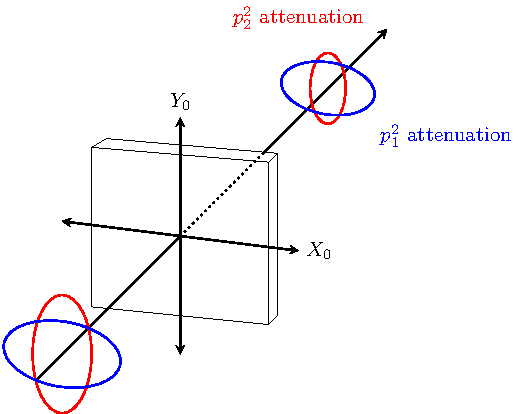
\includegraphics[scale=1]{images/theory/tikz_horizontal_diattenuator.pdf}
    \caption{Elliptical diattenuator at an angle of \SI{0}{\degree} to its intrinsic frame also known as a horizontal diattenuator. In this case the axes of the diattenuator align with the mayor and minor axis of its eigenstates so that the two eigenstates $\bm{\mathcal{E}}_1$, $\bm{\mathcal{E}}_2$ directly experience an intensity attenuation of $p_1^2$ and $p_2^2$, respectively.}
    \label{fig:horizontal_diattenuator}
\end{figure}

A diattenuator which is characterized by circular eigenstates, so that $\chi=\frac{\pi}{4}$ and therefore $\delta=\frac{\pi}{2}$, $\alpha=\frac{\pi}{4}$, is represented by the following Jones matrix:
\begin{equation}
    \hat{T}_{DC}(p_1, p_2) = \hat{T}_D\left(\frac{\pi}{4}, \frac{\pi}{2}, p_1, p_2\right) =
    \frac{1}{2}
    \begin{pmatrix} 
    p_1 + p_2 & -i(p_1 - p_2) \\
    i(p_1 - p_2) & p_1 + p_2
    \end{pmatrix}.
\end{equation}
It is worth noting that for $p_2=0$ $\hat{T}_{DC}(p_1, p_2=0)$ represents a circular polarizer which completely extinguishes the circular eigenstate $\bm{\mathcal{E}}_2$. The final of the three types is the linear diattenuator. In this particular case the eigenstates are linearly polarized so that $\chi=0$ and therefore $\delta=0$, $\alpha=\psi$. The linear diattenuator can accordingly be represented by the following Jones matrix:
\begin{equation}
    \hat{T}_{DL}(\psi, p_1, p_2) = 
    \begin{pmatrix} 
    p_1c_{\psi}^2 + p_2s_{\psi}^2 & c_{\psi}s_{\psi}(p_1 - p_2) \\
    c_{\psi}s_{\psi}(p_1 - p_2) & p_1s_{\psi}^2 + p_2c_{\psi}^2
    \end{pmatrix},
\end{equation}
which for $p_2=0$ represents the well known linear polarizer realized by for example a wiregrid polarizer. The Jones matrix then takes on the form:
\begin{equation}
    \hat{T}_{DL}(\psi, p_1, 0) = \hat{T}_{D}(\psi, 0, p_1, 0) =
    p_1
    \begin{pmatrix} 
    c_{\psi}^2 & c_{\psi}s_{\psi} \\
    c_{\psi}s_{\psi} & s_{\psi}^2
    \end{pmatrix}.
\end{equation}
It is worth noting that Malus' law can easily be derived from this, if we consider horizontally polarized light with an initial intensity $I_0=|E_x|^2$, as follows:
\begin{equation}
    \bm{\mathcal{E}}_{\SI{0}{\degree}}^{\dagger}
    \hat{T}_{DL}(\psi, p_1=1, 0)\bm{\mathcal{E}}_{\SI{0}{\degree}} = |E_x|^2p_1^2c_{\psi}^2 = I_0 c_{\psi}^2.
\end{equation}

Furthermore, oriented at \SI{0}{\degree} the horizontal diattenuator takes on the diagonal form $\hat{T}_{DL0}(p_1, p_2) = \hat{T}_{DL}(0, p_1, p_2)=\hat{T}_{D}(0,0,p_1,p_2)=\diag{p_1, p_2}$ and $\diag{p_1, 0}$ for a linear polarizer at $\psi = \SI{0}{\degree}$. Similar to the general form of the retarder, the elliptic diattenuator can also be written as a product of rotation matrices, horizontal retarders and diattenuators as follows:
\begin{align}
\begin{split}
    \hat{T}_{D}(\alpha, \delta, p_1, p_2) 
    &= \hat{T}_{RL0}(-\delta)\hat{T}_{DL}(\alpha, p_1, p_2)\hat{T}_{RL0}(\delta) \\
    &= \hat{T}_{RL0}(-\delta)\hat{Q}(-\alpha)\hat{T}_{DL0}(p_1, p_2)\hat{Q}(\alpha)\hat{T}_{RL0}(\delta).
\end{split}
\end{align}
This means that any diattenuator is equivalent to a linear diattenuator placed between two crossed linear retarders \cite{Gil2016}. 

\subsection{Diattenuating retarders - waveplates}
With the introduction of the diattenuator we can finally describe real linear retarders or specifically waveplates which in general show some amount of diattenuating effects \cite{D.CLARKE1971}. For this purpose we can assume that the optic axes of the retarder and diattenuator coincide, this assumption can be shown to be equivalent to the normality condition \cite{Bass1995}. Furthermore, we know from the previous section that states polarized along the fast or slow axis of the birefringent material of the waveplate will not undergo a polarization change as it passes through the waveplate. The eigenstates of a birefringent material are therefore linear and the planes of polarization coincide with the slow and fast axes of the material. Consequently, we can describe the waveplate using a linear retarder and diattenuator. A linear nonideal retarder or diattenuating retarder can be represented by the Jones matrix $\hat{T}_{RDL}$, which depends on four parameters; the orientation angle $\psi$ between the fast axis of the retarder $X_0$ and the axis $X$ of the reference frame, the principal intensities $p_1^2$ and $p_2^2$ and finally on the retardance $\Delta$. This means that $\hat{T}_{RDL}$ can be represented by the following product of matrices:
\begin{equation}
    \hat{T}_{RDL}(\psi, \Delta, p_1, p_2) = \hat{Q}(-\psi)\hat{T}_{RL0}(\Delta)\hat{T}_{DL0}(p_1, p_2)\hat{Q}(\psi),
\end{equation}
we can carry out the multiplication to obtain the following representation of $\hat{T}_{RDL}$:
\begin{equation}
    \hat{T}_{RDL}(\psi, \Delta, p_1, p_2) = 
    \begin{pmatrix} 
    p_1e^{i\Delta/2}c_{\psi}^2+p_2e^{-i\Delta/2}s_{\psi}^2 & c_{\psi}s_{\psi}\left(p_1e^{i\Delta/2}-p_2e^{-i\Delta/2}\right) \\
    c_{\psi}s_{\psi}\left(p_1e^{i\Delta/2}-p_2e^{-i\Delta/2}\right) & 
    p_1e^{i\Delta/2}s_{\psi}^2+p_2e^{-i\Delta/2}c_{\psi}^2
    \end{pmatrix}.
\end{equation}
This Jones matrix describes a single waveplate and a train of waveplates is then simply given by the product of the individual $\hat{T}_{RDL}$ matrices. Obtaining the retardance and diattenuation of the final product can be achieved with a polar decomposition, which states that for any complex 2x2 matrix $\hat{T}$ there exist positive-definite\footnote{A Hermitian matrix $\hat{H}$ is positive-definite if $\bm{\mathcal{E}}^{\dagger}\hat{H}\bm{\mathcal{E}}$ is positive for any $\bm{\mathcal{E}}$} Hermitian matrices $\hat{H}$ and $\hat{H}'$ and a unitary matrix $\hat{U}$ such that $\hat{T}=\hat{U}\hat{H}=\hat{H}'\hat{U}$. This means that an arbitrary Jones matrix describing any non-depolarizing optical element can be written as a product of a retarder and diattenuator as follows \cite{GilPerez2017}:
\begin{equation}
    \hat{T} = \hat{T}_R\hat{T}_D = \hat{T}_D'\hat{T}_R.
    \label{eq:diattenuation_retarder}
\end{equation}
Furthermore, the retardance $\Delta$ defined through the eigenvalues of $\hat{T}_R$ can be calculated using the following expression:
\begin{equation}
    \Delta = 2 \cos^{-1} \frac{\left|\tr\hat{T}+\frac{\det \hat{T}}{\left|\det \hat{T}\right|} \tr \hat{T}^{\dagger}\right|}{2\sqrt{\tr \hat{T}\hat{T}^{\dagger}+2\left|\det \hat{T}\right|}},
\end{equation}
which follows from the calculation of the eigenvalues of $\hat{T}$. We have to assume that the transmittances $p_1$ and $p_2$ are not zero since then $\hat{T}$ represents a polarizer for which the determinant of the corresponding Jones matrix is zero. Additionally, this equation is only valid for homogeneous Jones matrices. In the inhomogeneous case the following expression has to be used instead:
\begin{align}
\begin{split}
    \label{eq:retardation_inhomogeneous}
    \Delta &= 2\cos^{-1}\left\{r\left[\frac{(1-\eta^2)(|\lambda_q|+|\lambda_r|)^2}
    {(|\lambda_q|+|\lambda_r|)^2-\eta^2(2|\lambda_q||\lambda_r|+\lambda_q^*\lambda_r+\lambda_q\lambda_r^*)}\right]^{1/2}\right\}, \\
    r &= \left|\cos \frac{\delta_q-\delta_r}{2}\right|
\end{split}
\end{align}
where $\lambda_{r,q}=|\lambda_{q,r}|e^{i\delta_{q,r}}$ are the eigenvalues of $\hat{T}$.
Similarly, the diattenuation $D$ can be calculated from the Jones matrix as follows:
\begin{equation}
    \label{eq:diattenuation_2}
    D=\sqrt{1-\frac{4|\det \hat{T}|^2}{(\tr \hat{T}\hat{T}^{\dagger})^2}},
\end{equation}
which has the advantage that it does not depend directly on $p_1$ and $p_2$. Again, in the case of an inhomogeneous Jones matrix equation \ref{eq:diattenuation_2} is invalid and the following equation should be used:
\begin{equation}
    \label{eq:diattenuation_inhomogeneous}
    D=\sqrt{1- \frac{4(1-\eta^2)^2|\lambda_q|^2|\lambda_r|^2}
    {\left(|\lambda_q|^2+|\lambda_r|^2-\eta^2(\lambda_q\lambda_r^*+\lambda_r\lambda_q^*)\right)^2}}.
\end{equation}
Expressions \ref{eq:retardation_inhomogeneous} and \ref{eq:diattenuation_inhomogeneous} are valid for $\eta \neq 0$ but evidently less efficient \cite{Lu1994}. With this we can describe a train of waveplates and subsequently characterize the final Jones matrix through the equivalent retardance and diattenuation. In the following section we will consider the wavelength dependency of waveplates and introduce the achromatic waveplate (AWP), which ideally has the special property of being wavelength independent. 

\section{Achromatic waveplates}
\label{sec:achromatic_waveplates}

As we have seen already waveplates are highly wavelength sensitive due to the inverse wavelength dependency of the phase shift but also due to dispersion of the material refractive index and consequently dispersion of the birefringence. In other words the three parameters $\Delta$, $p_1$ and $p_2$ of the in total four parameters which define a linear diattenuating retarder or waveplate are wavelength dependent. There are several types of AWPs based on different techniques which can in theory compensate for this wavelength dependency. One possibility is to use the phase shift induced by total internal reflection which can be realized through a Fresnel Rhomb. Using this method it is possible to create an almost perfect AWP. The Fresnel Rhomb works over a large frequency range since the variation of retardance is solely due to the frequency dependent refractive index of the material used causing the reflectance to become wavelength dependent \cite{Hecht}. They often cause strong spatial shifts of the light, take up more space and are hard to align since the retardation strongly depends on the angle. Another method is to combine waveplates of different materials. The problem with this method is that only the dispersion of the materials is compensated for and so the resulting range is relatively low \cite{Masson2006}. The AWPs presented in this work are based on a similar design principle as the THz achromatic quartz quarter waveplates (TAQ) developed by Masson and Gallot in \cite{Masson2006}. The TAQ is ultimately based on the work by Destriau and Prouteau in 1949 \cite{Destriau1949} where they showed that the serial combination of a half waveplate and a quarter waveplate with an azimuth of $\SI{60}{\degree}$ results in a new achromatic quarter waveplate. This new AWP showed a $\frac{\pi}{2}$ phase shift over the whole visible range. Masson and Gallot extended this idea to the THz range by combining six quartz plates with variable thicknesses and again at different azimuths. This higher number of plates was necessary to cower a broader frequency range which is needed considering the typical bandwidth of typical THz-TDS systems. The operational principle of this type of AWP is based on the partial cancellation each plate is causing with respect to the frequency. Each quartz waveplate was assumed to have a negligible dichroism. It was reported that at \SI{1}{\tera \hertz} crystalline quartz showed an ordinary and extraordinary refractive index of $n_o=2.108$ and $n_o=2.156$, respectively. Due to this low birefringence the total thickness of the TAQ is relatively large. Assuming isotropic absorption of the plates, the AWP can be described by the following product:
\begin{equation}
    \hat{T}_{M} = \prod_{i=1}^{n=6} \hat{T}_{RL}(\psi_i, \Delta_i) = 
    \begin{pmatrix} 
    A & B \\
    -B^* & A^*
    \end{pmatrix},
    \label{eq:equiv_matrix}
\end{equation}
where according to equation \ref{eq:wp_eq} the $\Delta_i$ are proportional to the frequency and the thickness $d_i$ of the i-th waveplate. From the previous section we know that $\hat{T}_M$ can be written as the product of a diattenuator and a retarder. Therefore, setting $p_1=p_2=1$ and comparing the coefficients of $\hat{T}_{M}$ to a retarder represented by $\hat{T}_{RL}(\psi, \Delta_M)$ they get an expression for the so called resulting retardation dephasing $\Delta_M$:
\begin{equation}
    \label{eq:retardation_dephasing}
    \tan^2 \frac{\Delta_M}{2} = \frac{\operatorname{Im}A^2+\operatorname{Im}B^2}
    {\operatorname{Re}A^2+\operatorname{Re}B^2}.
\end{equation}
It is worth noting that the value $\Delta_M$ is not the same as the retardance defined in equation $\ref{eq:jones_ret_def}$. Nevertheless, it can be understood as the phase shift induced by a linear retarder $\hat{T}_{RL}(\SI{45}{\degree}, \Delta_M)$ on a horizontal state. The problem of determining the parameters $\psi_i$ and $d_i$ to get the appropriate phase shift at each frequency can be formulated as an optimization problem where the objective is to minimize the following error function:
\begin{equation}
    \label{eq:mass_loss}
    L(\psi_i, d_i)_M=\sum_{\nu}\left(\Delta_M(\nu)-\frac{\pi}{2}\right)^2.
\end{equation}
They minimize $L(\psi_i, d_i)_M$ using a simulated annealing algorithm over the frequency range \SIrange{0.2}{2}{\tera \hertz} and their result is shown in table \ref{tab:masson_result}. For this set of parameters it is reported that the deviation of $\Delta_M$ from $\frac{\pi}{2}$ is less than \SI{3}{\percent} over the frequency range \SIrange{0.25}{1.75}{\tera \hertz} and that the total thickness of the TAQ is \SI{31.4}{\milli \meter}. However they assume that the dichroism of the material is small enough to be negligible and it is therefore unaccounted for in the model. 

\begin{table}[h]
    \centering
    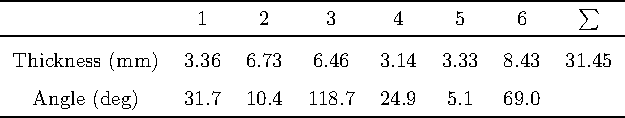
\includegraphics[scale=1]{images/theory/masson_result_table.pdf}
    \caption{Optimization result obtained by Masson and Gallot in \cite{Masson2006}. This particular TAQ consists of six plates of varying thicknesses and orientation angles.}
    \label{tab:masson_result}
\end{table}

A similar AWP is presented in another work by Wu, et al. Here they use sapphire instead of crystalline quartz which reduces the overall thickness of the AWP to \SI{2.453}{\milli \meter} since compared to quartz sapphire has a higher birefringence. They report a value of 3.39 and 3.07 for the ordinary and extraordinary refractive index, respectively. Similarly, they optimize the loss function given in equation \ref{eq:mass_loss} and by stacking even up to 20 individual plates they obtain a theoretical deviation of less than \SI{0.5}{\percent} from the $\pi/2$ target over the frequency range \SIrange{0.2}{2.0}{\tera \hertz}. Table \ref{tab:wu_result} shows their obtained values for the result with an overall thickness of \SI{2.453}{\milli \meter} consisting of six plates. The theoretical deviation of this result was around \SI{2.5}{\percent} and \SI{1}{\percent} for frequencies in the range \SIrange[range-phrase=-, range-units=single]{0.2}{0.5}{\tera \hertz} and \SIrange[range-phrase=-, range-units=single]{0.5}{2.0}{\tera \hertz}, respectively.
This design was produced and the phase shift was measured in the range from \SIrange{0.1}{0.8}{\tera \hertz}. However, the determined phase deviation exceeded \SI{3}{\percent} and even reached \SI{6}{\percent} at \SI{0.3}{\tera \hertz} which was a threefold increase compared to the optimization result. They attributed this deviation to angle misalignment and a mismatch between the used values from the actual values of the index of refraction of sapphire \cite{Wu2020}.

\begin{table}[h]
    \centering
    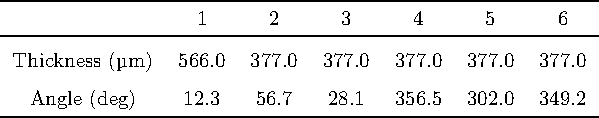
\includegraphics{images/theory/wu_result_table.pdf}
    \caption{Obtained parameters for $n=6$ published in \cite{Wu2020} with a design similar to that of Masson and Gallot. The higher birefringence of sapphire compared to quartz allows the plates to be thinner compared to the result by Masson and Gallot.}
    \label{tab:wu_result}
\end{table}

The realization of the AWP by Wu et. al \cite{Wu2020} resulted in a slightly worse performance compared to Masson et. al. \cite{Masson2006} for the quarter wave plate. However, the main advantage of the Wu et. al AWP was the use of a material with a higher birefringence which allowed them to reduce the thickness of their AWP by an order of magnitude. Furthermore, they used a different optimization algorithm, which we use for the optimization of our design. Finally, in both cases the absorption and diattenuation of the used materials were considered to be negligible and therefore also not considered in the AWP design.

The effect of dichroism on the performance of waveplates and the necessity to consider it when optimizing the design can be explained on an example of monochromatic $\lambda/2$ waveplates presented by Ornik et al. \cite{Ornik2018}. Four waveplates were produced by using selective laser-induced etching to fabricate waveplates with the periodically stratified structure as the media discussed at the end of section \ref{sec:wave_prop}. In simple words, from rectangular slab of fused silica glass, parts of glass were removed resulting in a series of glass bars separated by air grooves. Among other characterizing measurements the transmitted intensity of the waveplates were measured after passing a linear polarizer for different azimuths $\psi$. We know from equation \ref{eq:l2_wp_effect} that the effect of a $\lambda/2$ retarder is to rotate the mayor axes of the polarization ellipse by $-2\psi$. Therefore, if the input state is $\bm{\mathcal{E}}_{\SI{45}{\degree}}$ we expect a minimum in the transmitted intensity since then the output state is perpendicular to the transmission axis of the polarizer. This is of course only true for the frequencies where the retardance of the plate is $\pi$. In fact, if we assume the polar decomposition of the waveplate is a linear diattenuating retarder then we can show\footnote{See section \ref{sec:transmission_min} of the appendix} the following equation for the azimuth of the minimum transmittance:  
\begin{equation}
    \psi_{min}=\arctan\left(\sqrt{\frac{p_2}{p_1}}\right)
\end{equation}
Therefore, only if $p_1=p_2$ do we get the minimum transmittance at an azimuth of \SI{45}{\degree}. Although measurements of the intensity at different azimuths showed that the minimum transmission is not obtained for $\psi=\SI{45}{\degree}$ but rather at \SI{46}{\degree}, \SI{46}{\degree}, \SI{47}{\degree}, \SI{49}{\degree} for increasing thickness of the four waveplates. The work by Ornik et al. \cite{Ornik2018} therefore shows that in the case of form birefringent fused silica glass waveplates and waveplates consisting of anisotropic materials dichroism should be taken into consideration to obtain a better performing waveplate. In turn, this means that we cannot simply rely on optimizing the retardance to obtain designs which produce pure output polarizations. 

Building onto the method of Masson and Wu we therefore need to implement new loss or objective functions for the $\lambda/4$ and $\lambda/2$ waveplate types if we want to take dichroism into account. At the same time the form birefringent AWP type allows us to directly optimize the birefringence of each individual plate, but it also comes with the cost of adding $2n$ more degrees of freedom to the optimization problem. To summarize, the proposed AWP design consists of $n$ individual form birefringent plates where each plate has a similar structure as the one shown in figure \ref{fig:SLE_waveplate_JO_}. Similar to the TAQ waveplate, each individual plate is oriented at an azimuthal angle $\psi_i$ relative to the mayor axes of the polarization ellipse of the initial input state. Furthermore, each plate has a thickness $d_i$ and widths $a_i$ and $b_i$ of the stratification. If not stated otherwise $a_i$ and $b_i$ denote the width of the material bars and air grooves, respectively. The Jones matrix describing this configuration is therefore given by the following product:
\begin{equation}
    \hat{T}_{AWP}(\nu) = \prod_{i=1}^{n} \hat{T}_{RDL}(\psi_i, \Delta_i(\nu), p_{1,i}(\nu), p_{2,i}(\nu)),
\end{equation}
where the $\Delta_i$ are given by equation \ref{eq:wp_eq} which directly depends on $d_i$, the frequency $\nu=\frac{c}{\lambda}$ and the birefringence $\Delta n(\nu) = |n_o(\nu) - n_e(\nu)|$. Since the latter is approximated by equation \ref{eq:form_bf} $\hat{T}_{RDL}$ ultimately depends on $a_i$ and $b_i$ as well but only in case of form birefringent waveplates. Otherwise the birefringence is obtained from a measurement. This means that each plate has four free parameters in case of form birefringent waveplates. Since this already yields a fairly complex loss function we simplified the model by only considering dichroism and not first order reflection losses at the interfaces during optimization. The parameters $p_{j,i}$ are therefore simply the amplitude absorption losses along the principal axes of the plates, given by the imaginary parts of the calculated dielectric tensor coefficients. In the following we propose two objective functions which we optimized to obtain the results presented in the next chapter. In case of the objective function associated with the $\lambda/4$ waveplate type we optimize the components of the output state. Considering a $\bm{\mathcal{E}}_{\SI{0}{\degree}}$ input state then a $\lambda/4$ waveplate with its principal axes oriented at \SI{45}{\degree} relative to the input orientation should convert the input into a circularly polarized output. In general we get the following for a HLP input:
\begin{equation}
    \bm{\mathcal{E}}_o = \hat{T}_{AWP}\bm{\mathcal{E}}_{\SI{0}{\degree}} =
     \begin{pmatrix} T_{1,1} \\ T_{2,1} \end{pmatrix}.
\end{equation}
Circularly polarized states have the property that one component is real and the other imaginary. We use this to obtain the following loss function associated with the $\lambda/4$ waveplate:
\begin{equation}
\label{eq:l4_loss_function}
    L_{\lambda/4}(\bm{\psi}, \bm{d}, \bm{a}, \bm{b})=
    \sum_{\nu}\operatorname{Re}\left(r\right)^2+\left(1-\operatorname{Im}\left(r\right)\right)^2,
\end{equation}
with $r=\frac{T_{1,1}}{T_{2,1}}$ and $\bm{\psi}=\psi_1, ..., \psi_n$, $\bm{d}=d_1, ..., d_n$, etc. In other words we optimize the set of parameters so that $\bm{\mathcal{E}}_o=\bm{\mathcal{E}}_{LCP}$.
Even though we did not directly use it in this work we propose an objective function for the $\lambda/2$ waveplate based on the condition that $\hat{T}_{AWP}$ should act on an input state like $\hat{T}_{1/2}(\psi=\frac{\pi}{4})$ does. In other words, a LHP state transforms into a LVP state and in the case of non-linear states the handedness is inverted. We therefore optimize the parameters to fulfill the condition that $\hat{T}_{AWP}=\hat{T}_{1/2}(\psi=\frac{\pi}{4})$. With this the loss function to be optimized in case of the $\lambda/2$ waveplate is given by the following expression:
\begin{align}
\begin{split}
    L_{\lambda/2}(\bm{\psi}, \bm{d}, \bm{a}, \bm{b})=
    &\sum_{\nu}|T_{1,1}|^2+|T_{2,2}|^2\\
    +&\sum_{\nu}(1 - \operatorname{Im}(T_{1,0}))^2+
    (1 - \operatorname{Im}(T_{1,2}))^2,
\end{split}
\end{align}
in other words we directly optimize the coefficients of the Jones matrix describing the train of waveplates to be similar to the $\hat{T}_{1/2}$ Jones matrix.

In summary, we proposed a composite AWP design consisting of a number of stacked form birefringent waveplates. We additionally proposed two similar objective functions based on the Jones calculus which can be optimized in order to obtain the parameters for a $\lambda/2$ or a $\lambda/4$ AWP design. For verification we optimized the $\lambda/4$ objective function and realized the resulting design via a 3D printed structure which we subsequently characterized. The setups used for the characterization are presented in the following chapter and in the subsequent chapter the results are shown.

% while for the $\lambda/2$ type we directly optimize the coefficients of the Jones matrix describing the train of waveplates


\chapter{Experimental setups}
\label{ch:setups}
In this work three different setups were used in transmission geometry to obtain the permittivity of the materials in question and to characterize the waveplates. Each setup implements a different emitter-detector pair which in turn means that the frequency region with the maximum SNR varies depending on the setup. The frequency range in which we can reliably extract the optical parameters therefore varies depending on the setup. 

\section{THz-TDS TeraWave setup}
The THz-TDS TeraWave system is based on an erbium doped \SI{1560}{\nano \meter} \SI{60}{\milli \watt} fiber laser with a repetition rate of \SI{100}{\mega \hertz} and a pulse width of around \SI{80}{\femto \second}. The output of the laser is split by a 50/50 fiber splitter into a detector and emitter branch, each branch is then subsequently coupled into one of two mechanical delay stages. These components are all housed in a sealed box which further has two fiber interfaced outputs for the optical pulses, a voltage supply for the antenna bias as well as an ethernet connection used for data collection. The two delayed laser outputs can then be fed to the emitter-detector module pair via fibers. For the THz generation and detection two photoconductive \ce{InGaAs} switches are integrated in the modules. Specifically the emitter module consists of a \SI{100}{\micro \meter} stripline antenna with a \SI{120}{\volt} unipolar bias \cite{Vieweg2014}. %Whereas the detector module consists of a \SI{25}{\micro \meter} dipole antenna with a \SI{\pm 3}{\volt} bias. How do I cite that thing on the server???

The detector/emitter modules are further integrated into the measurement setup shown in figure \ref{fig:3_THz-TDS-HHI} (a). All shown components are contained in a sealed box which makes it possible to purge the environment with nitrogen to avoid absorption by water vapor contained in the air. The setup consists of four off-axis parabolic mirrors (OAPM) and a rotational sample holder shown in subfigure (b) which is further mounted to a mechanical stage. If not stated otherwise all measurements conducted using this setup were performed by placing the sample into the focus plane between the second and third OAPM, which first focus and then collimate the THz radiation. The mechanical stage allows us to move the sample out of the THz beam for reference measurements without releasing the nitrogen. A measurement with a wiregrid polarizer showed that the polarization of the emitted THz radiation is mainly linearly horizontally polarized relative to the optical table, this is indicated by the blue arrow. Using this setup the birefringence of a sample can be characterized by rotating sample mount with the sample.

\begin{figure}[H]
    \centering
    \subcaptionbox{\label{fig:1}}
        {\hspace*{-2em}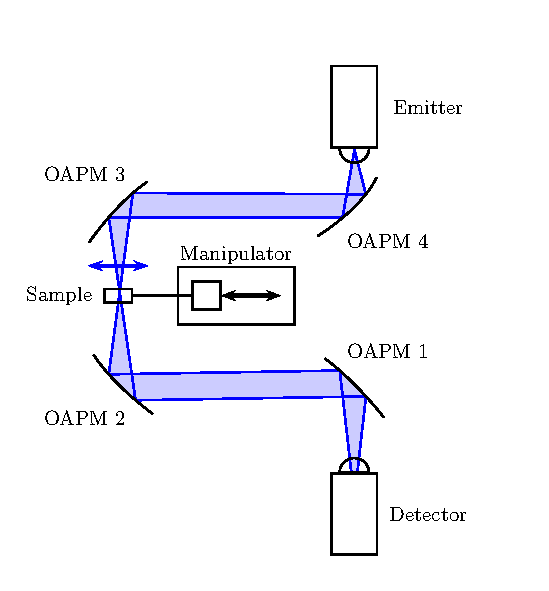
\includegraphics[width=0.45\linewidth]{images/setup/Setup-THz-TDS-HHI.pdf}}
    \qquad
    \subcaptionbox{\label{fig:2}}
        {\hspace*{-2em}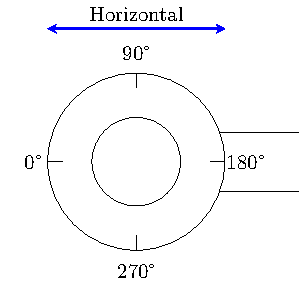
\includegraphics[width=0.45\linewidth]{images/setup/sample_mount_simple_nosample.pdf}}
    
    \caption{(a) The main components of the measurement setup which consists of four off-axis parabolic mirrors, the sample mounted on a translation stage (Manipulator) as well as the emitter and detector. (b) The rotational sample mount where the blue arrow indicates the horizontal direction which is also the polarization plane of the incident radiation.}
    \label{fig:3_THz-TDS-HHI}
\end{figure}

\begin{figure}
\centering
\subcaptionbox{\label{fig:circ_pol_planewave_a}}
    {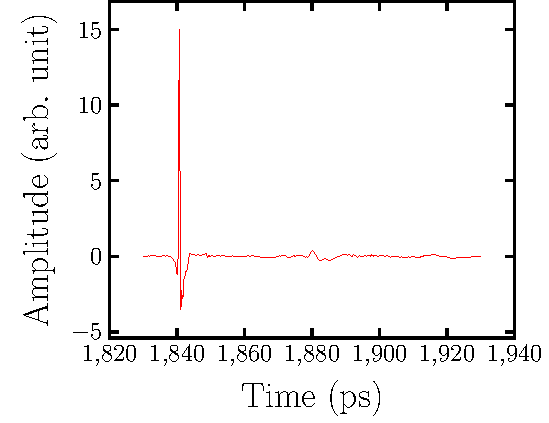
\includegraphics[scale=0.7]{images/setup/plots/pulse_example_a.pdf}}
\subcaptionbox{\label{fig:circ_pol_planewave_b}}
    {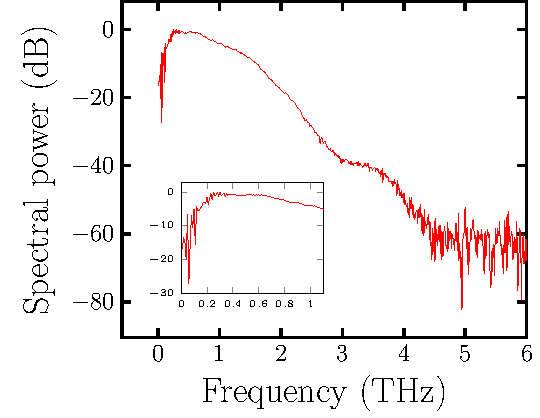
\includegraphics[scale=0.7]{images/setup/plots/pulse_example_b.pdf}}
\caption{(a) Example of a THz pulse from a reference measurement with 100 averages. (b) Spectrum of the pulse. The inset shows the first \SI{1}{\tera \hertz} of the spectrum with a bandwidth of around \SI{4.5}{\tera \hertz} and a signal peak at around \SI{500}{\giga \hertz}.}
\label{fig:HHI_pulse_example}
\end{figure}

Figure \ref{fig:HHI_pulse_example} (a) shows the time-domain signal from a \SI{100}{\pico \second} long reference measurement which consists of 100 averages recorded at \SI{80}{\milli \second} per trace. Figure \ref{fig:HHI_pulse_example} (b) shows the spectrum of the pulse. We see that the spectrum contains frequency components up to around \SI{4.5}{\tera \hertz} with a signal peak at around \SI{500}{\giga \hertz}. Below around \SI{200}{\giga \hertz} the signal becomes quite noisy. Additionally, we see that with an average of 100 traces the peak dynamic range for this setup is around \SI{60}{\decibel}.

\section{THz-TDS bow-tie setup}
\label{sec:bow_tie_setup}
The second THz-TDS system we used in this work is shown in figure \ref{fig:THz_bowtie_setup}. For this system again an Er:Fiber laser with an average power of around \SI{80}{\milli \watt} is used. The laser generates \SI{90}{\femto \second} pulses with a central wavelength of \SI{1560}{\nano \meter} at a rate of \SI{100}{\mega \hertz}. The laser output is first attenuated using a \SI{3}{\decibel} attenuator and then split into two branches using a 50/50 fiber splitter; one branch is coupled directly into the emitter while the other part is coupled into free-space and subsequently guided via mirrors (M1-3) over a mechanical delay line to a fibercoupler which is connected to the detector. Therefore, one major difference of this setup compared to the previously described one is that the mechanical delay line is not enclosed in a separate container. Additionally, different from the TeraWave setup the detector and emitter in this setup are employing bow-tie antenna structures. Another difference is that an AC voltage of \SI{20}{\volt} with a frequency of \SI{6346}{\hertz} is generated and applied to the emitter module. The current signal generated by the detector module is in the \si{\nano \ampere} range, therefore to distinguish and extract it from the background noise a lock-in amplifier is used. The generated AC \SI{6346}{\hertz} bias is further used as a reference by the lock-in amplifier.

In this setup we placed the sample in between two polyethylene lenses which were used to collimate the beam. Similarly to the previous setup we determined the polarization of the THz beam using a wire grid polarizer. The measured transmittance at different angles showed that the radiation was again mostly horizontally linearly polarized which is indicated by a blue arrow in figure \ref{fig:THz_bowtie_setup}. Figure \ref{fig:BT_pulse_example} (a) shows a reference measurement which consists of a single \SI{200}{\pico \second} trace; no averaging is performed due to the slower mechanical delay line compared to the delay line used in the TeraWave system and a single trace takes around \SI{150}{\second} to complete. Subfigure (b) shows the spectrum of the pulse. We see that the bandwidth of this setup is around \SI{700}{\giga \hertz} with a signal peak around \SI{200}{\giga \hertz}. However, it is not possible to purge the beam path in this system with nitrogen, which be seen by the existence of the water vapor absorption line around \SI{0.555}{\tera \hertz} \cite{VanExter1989}. Fortunately for this setup water vapor absorption is less a problem since the absorption of water vapor increases with frequency \cite{Series2019}. It is worth noting that the lower signal peak is useful in cases where the wavelength should be larger compared to the structural periodicity of the sample, which is why we use this system.

\begin{figure}[H]
    \centering
    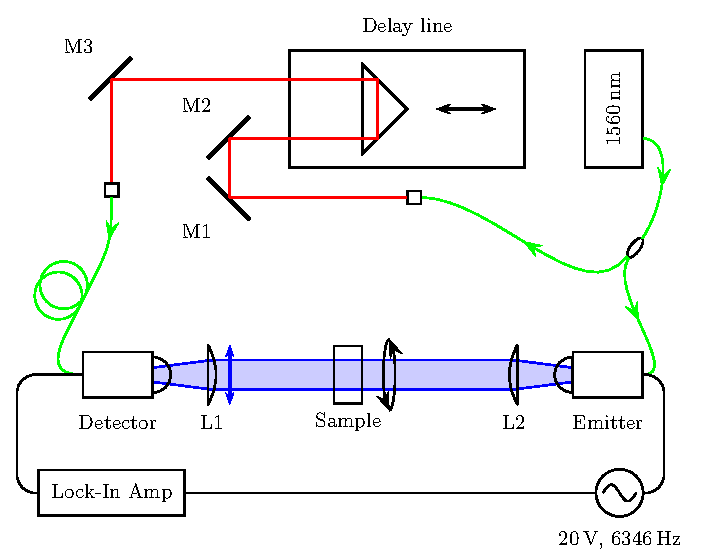
\includegraphics{images/setup/Setup-THz-TDS-Lab1.pdf}
    \caption{Schematic of the THz-TDS free-space setup. The \SI{1560}{\nano \meter} laser pulses are split into a detector branch and an emitter branch. Pulses in the detector branch are delayed by a mechanical delay line and serve as optical switches for the detector. The emitter is further modulated by a \SI{20}{\volt} \SI{6346}{\hertz} bias which is used as a reference by the lock-in amplifier to separate the detector signal from background noise. In this setup the THz beam is collimated and horizontally linearly polarized as indicated by the blue arrow.}
    \label{fig:THz_bowtie_setup}
\end{figure}

\begin{figure}[H]
    \begin{subfigure}[b]{.5\linewidth}
    \caption{}\label{}
    \centering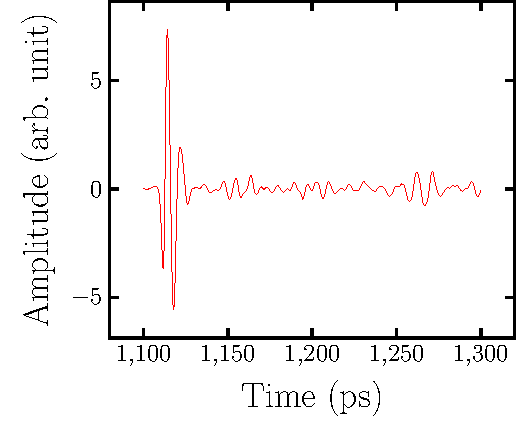
\includegraphics[scale=0.58]{images/setup/plots/pulse_example_bt_a.pdf}
    \end{subfigure}%
    \begin{subfigure}[b]{.5\linewidth}
    \caption{}\label{}
    \centering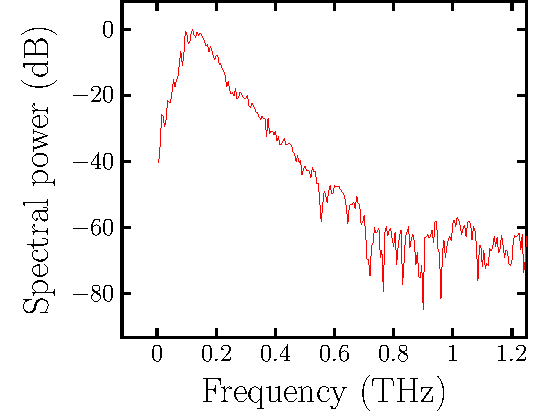
\includegraphics[scale=0.58]{images/setup/plots/pulse_example_bt_b.pdf}
    \end{subfigure}
    \caption{(a) Example of a THz pulse from a single \SI{200}{\pico \second} long reference measurement. (b) Spectrum of the pulse, which shows a bandwidth of around \SI{700}{\giga \hertz} with a signal peak around \SI{200}{\giga \hertz}}
    \label{fig:BT_pulse_example}
\end{figure}

\section{Quasi-optical GHz setup}
\label{sec:GHz_setup}
The rapid drop-off in spectral power at lower frequencies which we see for the two previously described setups show that especially at the lower end of the THz range high resolution measurements are difficult to perform with conventional THz-TDS setups. Additionally, for the characterization of form birefringent stratified structures with spatial periods in the lower millimeter range setups with higher resolution and SNR in the millimeter wavelength range are better suited. These samples were characterized by the High Frequency and Electromagnetic Fields group which is a department of the Physikalisch-Technische Bundesanstalt located near Braunschweig\footnote{\url{https://www.ptb.de/cms/en/ptb/fachabteilungen/abt2/fb-22.html}} since we do not have access to such setups; all measurements with the quasi-optical GHz setup (GHz setup) were therefore performed by this group.

For the characterization they used a free-space quasi-optical setup based on a vector network analyzer (VNA). A schematic of the setup is shown in figure \ref{fig:GHz_setup}, it mainly consists of a commercial VNA and different waveguide frequency extension unit sets. The frequency extension units allow the frequency range of the measurement to be converted into one of the following six ranges: \SIrange[range-phrase=--]{50}{75}{\giga \hertz}, \SIrange[range-phrase=--]{75}{110}{\giga \hertz}, \SIrange[range-phrase=--]{110}{170}{\giga \hertz}, \SIrange[range-phrase=--]{140}{220}{\giga \hertz}, \SIrange[range-phrase=--]{220}{325}{\giga \hertz} and from \SIrange{325}{500}{\giga \hertz}. We chose the range \SIrange{75}{110}{\giga \hertz} since it is wider than the range starting at \SI{50}{\giga \hertz} and the wavelength in this range is \SIrange{2.7}{4.0}{\milli \meter} which is still well into the \si{\milli \meter} range. 

\begin{figure}[H]
    \centering
    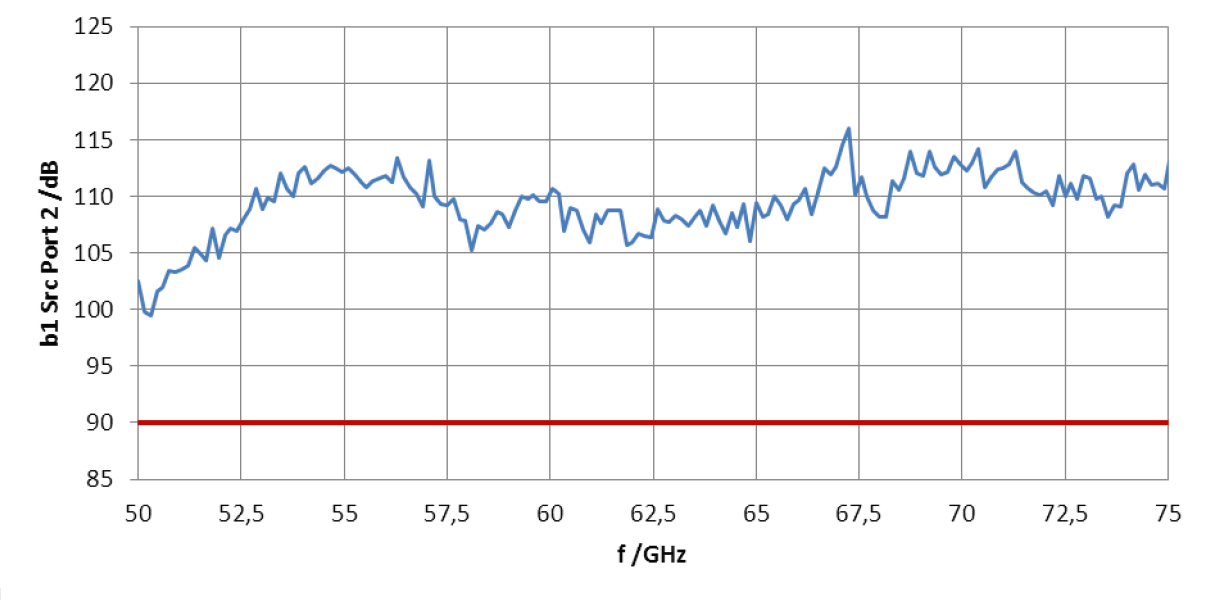
\includegraphics[scale=0.4]{images/setup/DNR.png}
    \caption{Dynamic range in dB versus frequency of the VNA combined with the \SIrange[range-phrase=--]{75}{110}{\giga \hertz} frequency extender. Source: \cite{VNADNR2013}}
    \label{fig:VNA_DNR}
\end{figure}

Furthermore, the waveguide ports of the frequency extenders are connected to two rectangular horn antennas and two OAPMs are used to reduce transmission losses. It is worth noting that similarly to the PCAs, conventional horn antennas also have a linear emission pattern \cite{ShiChen2013}. With this setup we get a frequency resolution of \SI{25}{\mega \hertz} while in case of the THz-TDS systems we get a resolution of \SI{5}{\giga \hertz} for a trace length of \SI{200}{\pico \second}. Figure \ref{fig:VNA_DNR} shows the dynamic range of the VNA and selected frequency converter system. We see that compared to the THz pulses the VNA has a fairly flat spectrum \cite{VNADNR2013, Kazemipour2015}.

\begin{figure}[H]
    \centering
    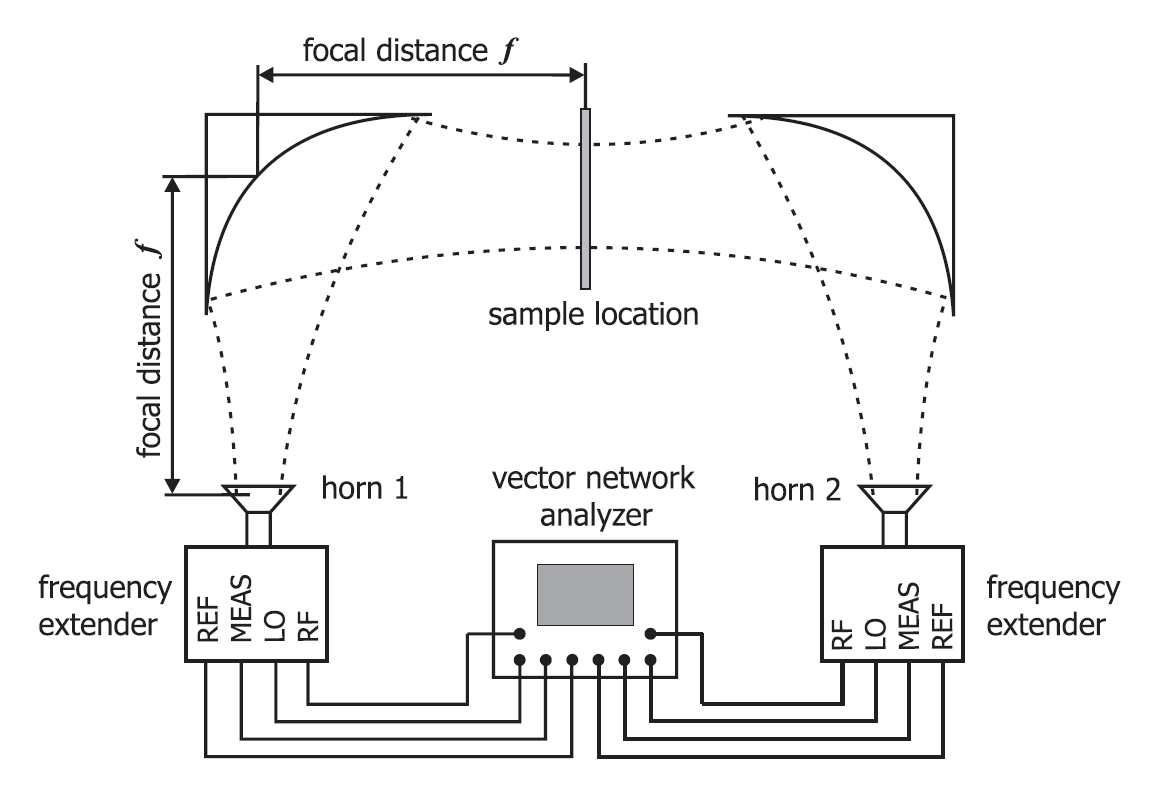
\includegraphics[scale=0.4]{images/setup/ghz.png}
    \caption{Schematic of the quasi-optical GHz setup. The vector network analyzer generates and measures the signal from which the S-parameters are obtained. A frequency extender enables the measurement to be performed from \SIrange{75}{110}{\giga \hertz}. Two OAPM reduce free-space transmission losses. Source: \cite{Kazemipour2015}}
    \label{fig:GHz_setup}
\end{figure}

The VNA measures the so called scattering parameters or S-parameters directly at each frequency. Simply put the S-parameters relate the EM-waves travelling towards and away from each antenna \cite{Caspers2012}. This means that if one considers the multiple reflections inside of the sample then they directly relate to the transmission and reflection coefficients of free space in combination with the sample. To extract the permittivity of the sample from the measured S-parameters, a reference measurement is therefore required. The reference measurement is performed without the sample in the beam path. The execution of the measurement and the extraction process is described in more detail in \cite{Kazemipour2015}. 


\chapter{Results}
Using the mathematical description and the optimization approach presented in chapter \ref{ch:wp_design} we present two different $\lambda/4$ AWP design types. The first design type aims at utilizing 3D printing of ceramic \ce{Al2O3} (alumina) for the fabrication of AWPs. The birefringence of 3D printed alumina is related to the printing process \cite{Ornik2021}. We rely on this reported birefringence and try to take advantage of this property to reduce the angular misalignment between individual plates forming the AWP. In the first section of this chapter results of two design optimizations for two different frequency ranges are presented. Furthermore, the two theoretical results are compared with the design reported by Masson et. al. \cite{Masson2006} and different parameters which can be used to describe the properties of the waveplates are discussed. Since the individual fabricated waveplates did not exhibit the expected birefringent values, the AWP was not assembled and experimentally characterized. The characterization of refractive index and absorption coefficient values of individual plates are shown in the Appendix section \ref{sec:ceramic_characterization}.

In the second section of this chapter the second design type is presented. This third result is based on form birefringence (see subsection \ref{sec:form_birefringence}). The goal of this part was to fabricate a stratified structure using a conventional low-cost polymer based 3D printer. Furthermore, an additional goal was to utilize 3D printing to avoid excessive angular misalignment of individual plates forming the AWP. However, the printing resolution of such low-cost 3D printers is limited and therefore this AWP was designed to work in the low THz or sub-THz range (\SIrange{75}{110}{\giga \hertz}). In this section first the design and expected AWP properties are presented. Then the experimental characterization of the AWP is shown and compared to the theoretical expectations. Finally the sources for the deviation between the theory and experiment are identified and discussed.

\section{Composite 3D printed ceramic AWP}
In a publication by Ornik et al. it was shown that \ce{Al2O3} as a 3D printed ceramic exhibited birefringent properties. A birefringence of approximately $0.05$ was reported for the range from \SIrange{0.25}{2.5}{\tera \hertz}. This value is fairly low compared to the birefringence of sapphire which is the crystalline form of \ce{Al2O3} with a birefringence of approximately $0.32$ \cite{Wu2020}. It was further shown that the direction of the slow axis was parallel to the printing direction. The sample is printed in two steps. In the first step, layer by layer is exposed to UV light which causes the polymerization in the slurry. This way the so-called green body is formed, which is then placed in an electric furnace exposed to \SI{1700}{\celsius} for the debinding and sintering processes. During these processes the sample shrinks for about \SI{21}{\volpercent} mainly due to the polymer burn-out. 

Two cylindric samples were printed and characterized and the corresponding data are shown in figure \ref{fig:ri_abs} \cite{Ornik2021}. (a) shows the measured refractive index along the slow and fast direction for the two samples and the birefringence as a function of the frequency, while (b) shows the measured absorption coefficient for the two samples and directions as a function of the frequency. We see that within the error range the birefringence of the two samples is equal. Therefore, either set of sample parameters works for setting up the objective function, we choose to use the measurement result of sample 1. 

\begin{figure}[ht]
    \begin{subfigure}[b]{.5\linewidth}
    \caption{}\label{}
    \centering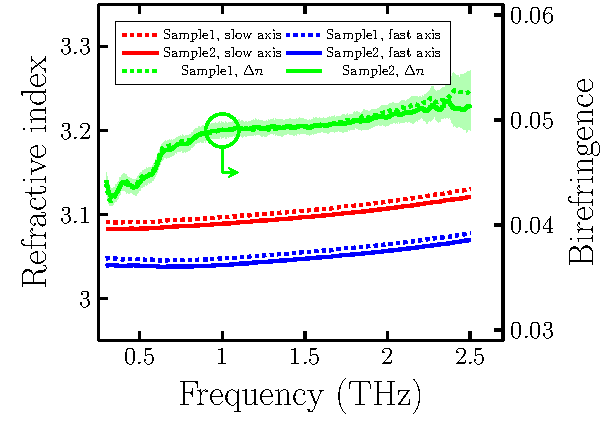
\includegraphics[scale=0.73]{images/results/plots/ceramic/ri_bf_a.pdf}
    \end{subfigure}%
    \hspace{3em}
    \begin{subfigure}[b]{.5\linewidth}
    \caption{}\label{}
    \centering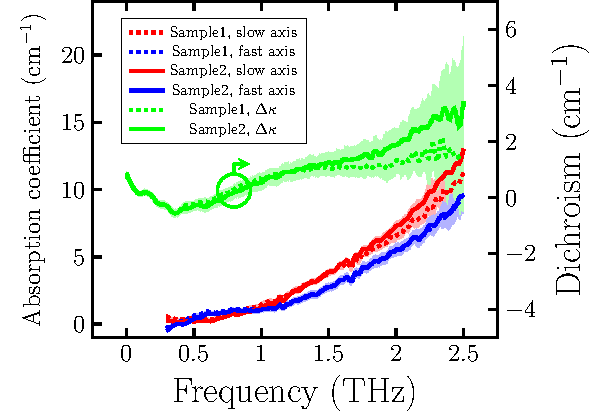
\includegraphics[scale=0.73]{images/results/plots/ceramic/ri_bf_b.pdf}
    \end{subfigure}
    \caption{(a) The refractive index and birefringence as a function of frequency for the two alumina samples; sample 1 and 2. For both samples the refractive index was measured for the perpendicular slow and fast axes. Considering the error margins both samples have an equal birefringence. (b) The absorption coefficient, again for the slow and fast axis of the samples. Data source: \cite{Ornik2021}}\label{fig:ri_abs}
\end{figure}

Stacking a number of these ceramic discs or plates we can in theory construct an AWP similar to the TAQ by Masson. This technique has the advantages that since the plates are 3D printed we can ideally control the thickness of the individual plates and also simplify the angular alignment. To do so, we considered printing cylindrical shaped samples with a flat side for easier orientation when stacking the individual plates. However, since the samples were printed standing directly on the platform without any support, the side of the sample in contact with the platform had to be also flat to ensure proper contact with the building platform. In figure \ref{fig:ceramic_stack} three plates of the described shape are shown and the idea of stacking the single plates at an orientation according to the optimized design.
%This ceramic AWP can then serve as a comparison to the TAQ and therefore also partly as a verification of the objective function at least for the $\lambda/4$ AWP type. In this case the objective functions $L_{\lambda/4}$ and $L_{\lambda/2}$ only depend on the set of angles and thicknesses. In other words the birefringence does not change at each iteration and is the same for each individual plate. A schematic of an AWP of this type consisting of three ceramic discs is shown in figure \ref{fig:ceramic_stack}. Each disc has two flat sides on the edge where one is used for alignment and the other is the printing base. The alignment flat is placed keeping in mind that the slow axis is along the printing direction. In reality the discs are stacked so that ideally there should be no air gaps in between each waveplate.

\begin{figure}[ht]
    \centering
    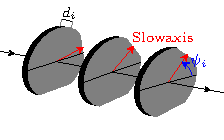
\includegraphics[scale=3.00]{images/results/tikz_wpstack_ceramic.pdf}
    \caption{Exploded view of a ceramic AWP with $n=3$. In general each waveplate has a thickness $d_i$ and an orientation angle or azimuth $\alpha_i$. The individual plates are printed with two flat sides; one is used to align the discs and the other serves as support during the printing process. The red arrow points to the supportive base which is therefore the printing direction and hence the slow direction.}
    \label{fig:ceramic_stack}
\end{figure}

%In order to reproduce the TAQ the birefringence is required which can obtained from the reported values in \cite{DGrischkowsky1990}, this is also the source used in \cite{Masson2006}. To this extend the Sellmeier equation allows us to interpolate the values in the reported data range which is from \SIrange{0.2}{2.0}{\tera \hertz}, details of the procedure can be found in the appendix section \ref{sec:sellmeier}. Using the thicknesses and angles of the TAQ given in table \ref{tab:masson_result} as well as the birefringence of quartz we can then calculate $L_{\lambda/4}(\nu)$ for the TAQ to use it for comparison. Furthermore, we optimized $L_{\lambda/4}$ for $n=6$ in the range from \SIrange{0.25}{1.50}{\tera \hertz}. The design parameters obtained from this optimization are shown in table \ref{tab:res_cl4} (Result 1). Additionally, the individual terms of $L_{\lambda/4}(\nu)$ of this result as well as those for the TAQ are plotted in figure \ref{fig:loss_function_cl4} as a function of frequency. We see that the magnitude of $L_{\lambda/4}$ for these two results is similar. Assuming that $L_{M}$ is a correct measure of the frequency dependent performance of the waveplate this means that $L_{\lambda/4}$ is also a suitable measure of the quality of the result. At around \SI{1.5}{\tera \hertz} there is a clear cut-off for Result 1 after which $L_{\lambda/4}$ increases steeply. This steep increase starts at around \SI{1.6}{\tera \hertz} for the TAQ. Defining the bandwidth as the ratio between the upper and lower frequency we get a value of  $\frac{\SI{1.5}{\tera \hertz}}{\SI{0.3}{\tera \hertz}}=5$. 

We optimized two designs which we call Result 1 and 2 for the frequency ranges \SIrange[range-phrase=-, range-units=single]{0.25}{1.50}{\tera \hertz} and \SIrange[range-phrase=-, range-units=single]{0.50}{2.25}{\tera \hertz}, respectively. In the work by Masson et al. the bandwidth of an AWP is defined as the ratio of the highest and lowest frequency in the range \cite{Masson2006}. Adopting this definition we have a bandwidth of around 5 and 6 for Result 1 and 2, respectively. The design parameters obtained from the optimization of the two results are listed in table \ref{tab:res_cl4}. 

\begin{table}[ht]
    \centering
    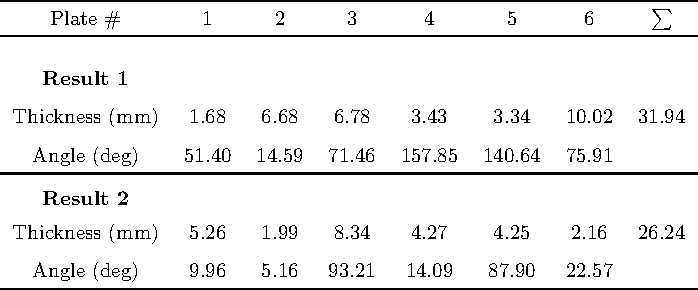
\includegraphics[scale=1.0]{images/results/ceramic_result_table.pdf}
    \caption{Design parameters for Result 1 and 2. Both results are obtained through the optimization of $L_{\lambda/4}$ for $n=6$. In the case of Result 1 the frequency range for the optimization was limited to \SIrange[range-phrase=-, range-units=single]{0.25}{1.50}{\tera \hertz} while for Result 2 the range was set to \SIrange[range-phrase=-, range-units=single]{0.50}{2.25}{\tera \hertz}.}
    \label{tab:res_cl4}
\end{table}

%\begin{figure}[H]
%    \centering
%    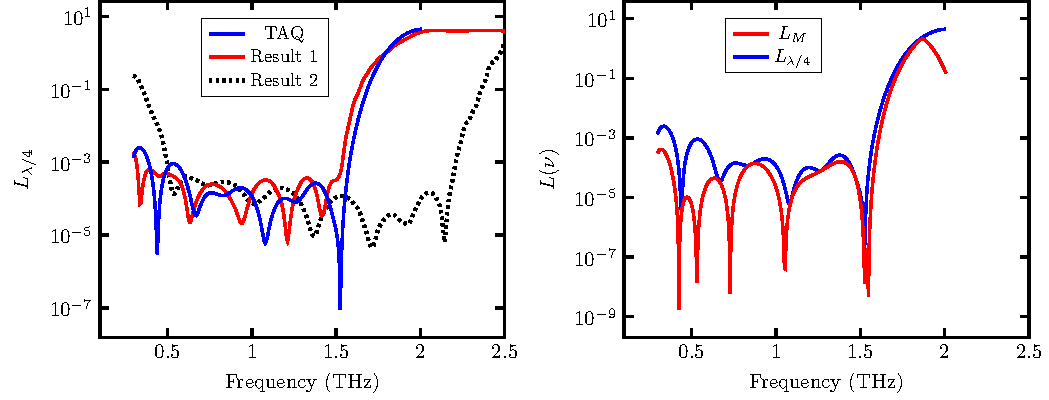
\includegraphics[scale=0.78]{images/results/plots/ceramic/loss_function.pdf}
%    \caption{The left subfigure shows the value of $L_{\lambda/4}$ as a function of frequency for the two results compared to the TAQ published in \cite{Masson2006}. We see that in the range in which the optimization took place the magnitude of $L_{\lambda/4}$ for the three results is fairly similar. The right subfigure shows the values of $L_M$ and $L_{\lambda/4}$ for the TAQ design with respect to the frequency. The largest difference between the two is around \SI{0.5}{\tera \hertz} and \SI{0.7}{\tera \hertz}, otherwise the trend of the two objective functions is relatively similar.}
%    \label{fig:loss_function_cl4}
%\end{figure}

The most notable difference we see between the two results is their total thickness. The total thickness of Result 1 is around \SI{32}{\milli \meter} while for Result 2 it is only around \SI{26}{\milli \meter}. However both results are fairly thick compared to the sapphire waveplate by Wu et al. \cite{Wu2020}. This is likely because similar to quartz, the birefringence of the ceramic plates is relatively low. This in turn means that for the waveplates to have an effect in the lower end of the spectrum the individual plates must be fairly thick, due to the proportionality between the phase shift and the frequency. Additionally, since the lower end of the optimized frequency range is slightly higher for Result 2 compared to Result 1 its total thickness is also slightly lower.
 
 We can calculate the thickness required to cause a quarter wave shift at the minimum of the frequency range for a linearly polarized input with an azimuth of \SI{45}{\degree}. In other words the thickness of a ceramic zero order quarter waveplate at the minimum frequency, this is given by equation $\ref{eq:thickness_quarter_waveplate}$. In this case the minimum frequency is \SI{0.25}{\tera \hertz}, at this frequency the birefringence is $\Delta n = 0.047$. The required thickness is therefore approximately $d_{\lambda/4}=\frac{\SI{1200}{\micro \meter}}{4\cdot0.047}=\SI{6.38}{\milli \meter}$. Comparing this value to the total thicknesses of the two results we see that it is several times smaller and almost \SI{4}{\milli \meter} thinner than the thickest plate. If we keep in mind that a probabilistic algorithm is part of the optimization method, then this could indicate that the obtained results are not the thinnest possible configurations for the given frequency ranges and material. On the other hand however, we have to keep in mind that $d_{\lambda/4}$ is for an angle of \SI{45}{\degree} while the six plates of the AWP are in general at different angles reducing the phase shift caused by each plate. It is therefore questionable whether we can actually directly compare $d_{\lambda/4}$ to the total thickness.

Furthermore, if we consider two results where the total thickness of the latter is larger, then the magnitude or intensity of the corresponding output state will in general be lower compared to the output of the first result. However, $L_{\lambda/4}(\nu)$ is insensitive to isotropic changes in the absorption. So if the ellipticity and orientation of the polarization ellipses corresponding to the two results are equal for all frequencies then $L_{\lambda/4}$ will attain the same value in both cases. In other words, $L_{\lambda/4}(\nu)$ is the same for two states $\bm{\mathcal{E}}$ and $p\bm{\mathcal{E}}$, $0<p<1$ for any frequency. The intensity coefficients $p_1^2$ and $p_2^2$ for the equivalent elliptic diattenuator Jones matrix describing the result with a larger total thickness will both be scaled by $p^2$. Since in the definition of $L_{\lambda/4}$ the elements of the Jones matrix enter as a ratio, the factor $p^2$ then subsequently cancels out and both results will attain the same value of $L_{\lambda/4}$. This in turn means that there is no direct penalty for increasing the thicknesses other than increasing the effect of dichroism.

To gain an estimate of the performance of the objective function and the optimization routine we compare the values of the objective function $L_{\lambda/4}$ with respect to frequency proposed in this work to the values of the one used by Masson et al.; $L_{M}$ given in equation \ref{eq:mass_loss} \cite{Masson2006}. We do this using the design parameters of the TAQ given in table \ref{tab:masson_result} as well as the optical parameters of quartz published in \cite{DGrischkowsky1990} which is also the source used by Masson et al. \cite{Masson2006}. However, since we do not have direct access to the measured data points we use the Sellmeier equation to interpolate the optical parameters of quartz in the reported data range which is from \SIrange{0.2}{2.0}{\tera \hertz}, details of the procedure can be found in the appendix section \ref{sec:sellmeier}. It is worth emphasizing that in contrast to $L_{\lambda/4}$ the dichroism is unaccounted for in the calculation of $L_{M}$. The comparison is shown in figure \ref{fig:loss_function_cl4_b}, i.e. the calculated values of the two objective functions $L_{\lambda/4}$ and $L_{M}$ for the design parameters of the TAQ given in table \ref{tab:masson_result}. We see that the shape of the two functions match fairly well except for some lower frequencies and especially at around \SI{0.55}{\tera \hertz} we see a larger deviation. 

\begin{figure}[H]
    \centering
    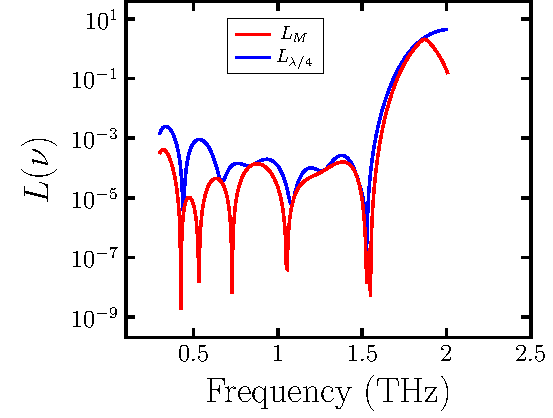
\includegraphics[scale=0.78]{images/results/plots/ceramic/loss_function_b.pdf}
    \caption{Values of $L_M$ and $L_{\lambda/4}$ for the TAQ design with respect to the frequency. The largest difference between the two is around \SI{0.5}{\tera \hertz} and \SI{0.7}{\tera \hertz}, otherwise the trend of the two objective functions is relatively similar.}
    \label{fig:loss_function_cl4_b}
\end{figure}

To address the question whether Result 1 is the global minimum or if there is a better suited one we plotted the minimum value of $\sum_{\nu}L_{\lambda/4}(\nu)$ as function of the current iteration step in figure  \ref{fig:cl4_convergence}. We see that the algorithm converges fairly fast and we only noticed major changes for approximately the first 25 iterations. This indicates that finding a solution with $n=6$ which performs significantly better in the range of \SIrange{0.25}{1.50}{\tera \hertz} is unlikely using the current algorithm and objective function.

\begin{figure}[H]
    \centering
    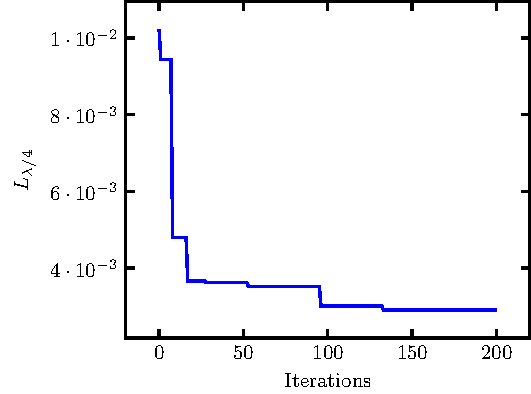
\includegraphics[scale=0.7]{images/results/plots/ceramic/convergence.pdf}
    \caption{Minimum value of $L_{\lambda/4}$ as a function of the total iteration count for the frequency range \SIrange{0.25}{1.5}{\tera \hertz} and a plate count of six. This shows that for the chosen settings the algorithm convergences rather fast.}
    \label{fig:cl4_convergence}
\end{figure}

This means that we can conclude $L_{\lambda/4}$ is a fairly good estimate of the performance of the AWP if we assume $L_{M}$ is as well. Additionally, the optimization routine converges to a local minimum of the objective function sufficiently fast. Therefore, the design procedure proposed in this work performs similarly to the one described in the work by Masson et al. with the addition that we consider dichroism as well. 

In the following we compare Result 1 and 2 based on the design parameters given in table \ref{tab:res_cl4} and 3D printed alumina to the quartz TAQ for which the parameters are listed in table \ref{tab:masson_result}. Both materials have a similar birefringence but the absorption and dichroism of alumina is significantly higher. We can therefore expect a similar performance in terms of polarization conversion between these two types but we also expect that the alumina AWPs cause higher losses. For this purpose the individual terms of $L_{\lambda/4}$ for the three designs are shown in figure \ref{fig:loss_function_cl4_a}, i.e. $L_{\lambda/4}(\nu)$ for each frequency, where the frequency range is bound by the available material data. We see that the magnitude of the values is similar in the optimized frequency range.

%The design parameters of Result 2 are given in the lower half of table \ref{tab:res_cl4} and the dotted line in the left subfigure of figure \ref{fig:loss_function_cl4} shows the individual terms of $L_{\lambda/4}$ for each frequency bound by the available material data range. The right subfigure shows a comparison between $L_M(\nu)$ and $L_{\lambda/4}(\nu)$ for the TAQ. We see that the shape of the two functions match fairly well except for the lower frequencies and especially at around \SI{0.55}{\tera \hertz} we see a larger deviation. 

\begin{figure}[H]
    \centering
    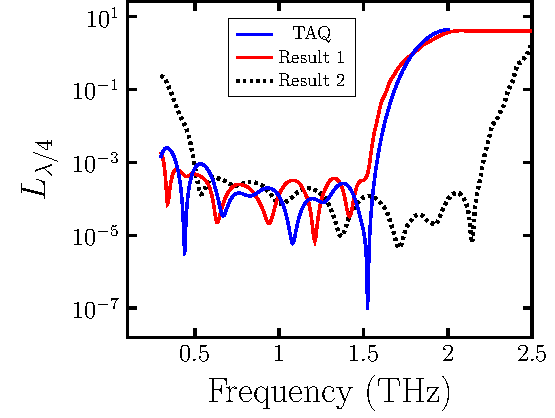
\includegraphics[scale=0.78]{images/results/plots/ceramic/loss_function_a.pdf}
    \caption{The value of $L_{\lambda/4}$ as a function of frequency for the two results compared to the TAQ published in \cite{Masson2006}. We see that in the range in which the optimization took place the magnitude of $L_{\lambda/4}$ for the three results is fairly similar.}
    \label{fig:loss_function_cl4_a}
\end{figure}

%Although, if we shift the frequency range of the optimization to \SIrange[range-phrase=-, range-units=single]{0.5}{2.25}{\tera \hertz} then we obtain a second result (Result 2) for which the bandwidth is almost five as well $\left(\frac{\SI{2.25}{\tera \hertz}}{\SI{0.5}{\tera \hertz}}=4.5\right)$. With that the total thickness of the AWP can be reduced to \SI{26}{\milli \meter} compared to the \SI{32}{\milli \meter} of Result 1. 

%The design parameters of Result 2 are given in the lower half of table \ref{tab:res_cl4} and the dotted line in the left subfigure of figure \ref{fig:loss_function_cl4} shows the individual terms of $L_{\lambda/4}$ for each frequency bound by the available material data range. The right subfigure shows a comparison between $L_M(\nu)$ and $L_{\lambda/4}(\nu)$ for the TAQ. We see that the shape of the two functions match fairly well except for the lower frequencies and especially at around \SI{0.55}{\tera \hertz} we see a larger deviation. 

In addition to considering the performance of the optimization procedure and objective function we can also compare the theoretical performance of the designs in terms of their polarization conversion effectiveness. For this purpose we discuss different properties of the final polarization state as a function of the frequency, where we assume initially HLP THz radiation if not stated otherwise.

Figure \ref{fig:cl4_alpha} shows $\alpha$ for the output state for Result 1 and the TAQ. Since $\alpha$ is a measure of the ellipticity of the output state it shows the difference between a circular shape and the shape of the output. For a circle $\alpha$ is $\arctan(1)=\SI{45}{\degree}$ which is therefore the target value. If we compare $\alpha$ for the TAQ and at the frequency \SI{0.55}{\tera \hertz} to $L_{\lambda/4}$ at the same frequency, we see that the large deviation from the optimum is correctly indicated by $L_{\lambda/4}$ while $L_M$ shows a minimum and thereby fails to recognize the deviation. We see the same situation at around \SI{0.75}{\tera \hertz}. 

\begin{figure}[H]
    \centering
    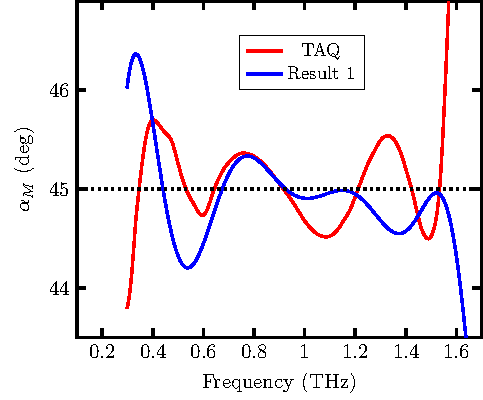
\includegraphics[scale=0.73]{images/results/plots/ceramic/alpha.pdf}
    \caption{$\alpha$ of the output state as a function of the frequency given a HLP input for the TAQ and Result 1. Ideally $\alpha$ should be equal to \SI{45}{\degree} independent of frequency. We see that the deviation of Result 1 from the optimum is distributed more evenly on the frequency range, while for the TAQ the deviation is higher at lower frequencies.}
    \label{fig:cl4_alpha}
\end{figure}

Comparing the values of $\alpha$ to figure \ref{fig:loss_function_cl4_b} and considering that the values of $L_M$ and $L_{\lambda/4}$ shown in figure \ref{fig:loss_function_cl4_b} are calculated from the same Jones matrix, we can also conclude that at least for some frequencies $L_{\lambda/4}$ is better at identifying deviations of the output from the optimal CP state. This could be due to the fact that the value of $L_{\lambda/4}$ is directly a measure of the difference between the state of the output and the RCP state.

%Considering that $L_M$ and $L_{\lambda/4}$ are calculated from the same Jones matrix, which is constructed from the parameters of the TAQ and crystalline quartz, figure \ref{fig:cl4_alpha} combined with figure \ref{fig:loss_function_cl4_b} shows that at least for some frequencies $L_{\lambda/4}$ is better at identifying deviations of the output from the optimal CP state. This could be due to the fact that the value of $L_{\lambda/4}$ is directly a measure of the difference between the state of the output and the RCP state.

\begin{figure}[H]
    \begin{subfigure}[b]{.5\linewidth}
    \caption{}\label{}
    \centering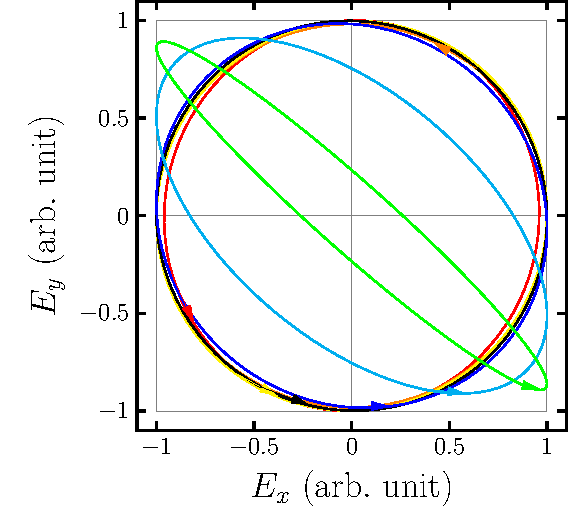
\includegraphics[scale=0.7]{images/results/plots/ceramic/pe_cl4_lp_a.pdf}
    \end{subfigure}%
    \begin{subfigure}[b]{.5\linewidth}
    \caption{}\label{}
    \centering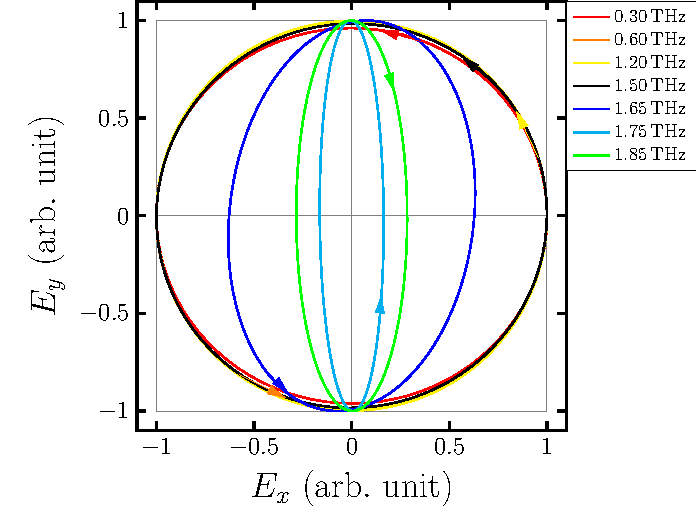
\includegraphics[scale=0.7]{images/results/plots/ceramic/pe_cl4_lp_b.pdf}
    \end{subfigure}
    \caption{Polarization ellipse representation of the output states for a HLP input at seven different frequencies. (a) The output of the TAQ. (b) The output of the ceramic AWP with the parameters from Result 1.}
    \label{fig:cl4_pe_lp}
\end{figure}

Figure \ref{fig:cl4_pe_lp} shows the polarization ellipses of the normalized states at seven different frequencies. The ellipses for the output of the TAQ is shown in (a) while (b) shows those for Result 1. The arrows indicate the handedness of the polarization. We see that as expected we get LCP states in the frequency range in which the optimization took place. Outside of that range the states are significantly more elliptical. We also see a slightly better result for the intermediate frequencies compared to the lowest at \SI{0.3}{\tera \hertz}. 

% TODO note starts to work as lambda half at higher freq. -> 90deg azimuth (nah)

\begin{figure}[H]
    \begin{subfigure}[b]{.5\linewidth}
    \caption{}\label{}
    \centering\includegraphics[scale=0.7]{images/results/plots/ceramic/pe_cl4_cp_a.pdf}
    \end{subfigure}%
    \begin{subfigure}[b]{.5\linewidth}
    \caption{}\label{}
    \centering\includegraphics[scale=0.7]{images/results/plots/ceramic/pe_cl4_cp_b.pdf}
    \end{subfigure}
    \caption{Polarization ellipse representation of the output states for a LCP input at seven different frequencies. (a) The output of the TAQ. (b) The ceramic AWP with the parameters from Result 1.}
    \label{fig:cl4_pe_cp}
\end{figure}

Figure \ref{fig:cl4_pe_cp} is similar to figure \ref{fig:cl4_pe_lp} except that the input in this case is LCP. In theory a quarter waveplate should produce a linearly polarized output for a circularly polarized input. We see that this is the case for the TAQ up to at least \SI{1.50}{\tera \hertz}, after which the state increasingly deviates from the linear ellipse shape. Interestingly the ellipses of Result 1 have a lower ellipticity compared to those of the TAQ, which indicates that the TAQ is better suited for turning a circularly polarized input into a linear polarized output. The reason for this could be that we only consider the circularity of the output state in the objective function used to obtain Result 1, while for the TAQ the resulting phase shift was directly optimized. This could therefore indicate that it is not sufficient to only consider the circularity of the output state in the objective function and a measure of the linearity or another appropriate property should be included as well. Although, on the other hand the relatively large deviation that can be seen at \SI{1.50}{\tera \hertz} can also be recognized in the plot of the objective function in figure \ref{fig:loss_function_cl4_a}. Which means that the deviation is recognized by the objective function but a minimum was not found that minimizes $L_{\lambda/4}$ at this frequency. This could therefore indicate that it is more difficult to minimize $L_{\lambda/4}$ compared to minimizing $L_M$.

The circular and linear polarization degrees $V_c$ and $V_l$ for a linearly polarized input state is shown in figure \ref{fig:cl4_pol_deg} as a function of frequency for Result 1 and the TAQ. Subfigures (a) and (c) show the full frequency range of $V_c$ and $V_l$, respectively, while subfigures (b) and (d) show the first \SI{1.6}{\tera \hertz}. For clarity $V_c$ is offset by one in (b) so that values of $V_c$ closer to zero are in fact closer to negative one. We see that as expected $V_c$ is around $-1$ in the optimization range for both the TAQ and Result 1 which indicates that the light is almost purely LCP. Interestingly, outside of the optimization frequency range the light switches to be primarily RCP. 

\begin{figure}[H]
\centering
\subcaptionbox{\label{fig:cl4_pol_deg_a}}
    {\hspace*{-2em}\includegraphics[width=0.41\linewidth]{images/results/plots/ceramic/polDeg/degCirc.pdf}}
\qquad
\subcaptionbox{\label{fig:cl4_pol_deg_b}}
    {\hspace*{-2em}\includegraphics[width=0.45\linewidth]{images/results/plots/ceramic/polDeg/degCircZoom.pdf}}
\subcaptionbox{\label{fig:cl4_pol_deg_c}}
    {\hspace*{-2em}\includegraphics[width=0.41\linewidth]{images/results/plots/ceramic/polDeg/degLin.pdf}}
\qquad
\subcaptionbox{\label{fig:cl4_pol_deg_d}}
    {\hspace*{-2em}\includegraphics[width=0.44\linewidth]{images/results/plots/ceramic/polDeg/degLinZoom.pdf}}
\caption{Subfigures (a) and (c) in the left column show the circular and linear polarization degrees, respectively, as a function of the frequency for Result 1 and the TAQ. Subfigures (b) and (d) in the right column also show the polarization degrees but for a smaller frequency range. The circular polarization degree in (b) is offset by one.}
\label{fig:cl4_pol_deg}
\end{figure}

Furthermore, subfigure (b) shows that $V_c$ for Result 1 varies less for frequencies below \SI{0.6}{\tera \hertz} and more for higher frequencies compared to the TAQ and varies less overall. This could be due to the difference between the refractive indices used for quartz during optimization and the values used for the calculation of $V_c$, since these deviations are fairly small. Subfigure (c) shows that the linear polarization degree increases to one and decreases again while the light switches to RCP. Subfigure (d) shows a similar trend as (b) in the sense that Result 1 is closer to zero at lower frequencies compared to the TAQ. We also see that $V_l$ is not zero, the light is therefore not perfectly CP but also partly LP, which is difficult to see in the polarization ellipse representation. 

Using the values for the absorption coefficient of quartz reported in \cite{DGrischkowsky1990} we can calculate the intensity of the light after passing through the \SI{31.45}{\milli \meter} thick TAQ. We can carry out the same calculation for the ceramic AWP designs; Result 1 and the slightly thinner Result 2 which have a total thickness of \SI{31.94}{\milli \meter} and \SI{26.24}{\milli \meter}, respectively. The transmission as a function of frequency for these three designs is shown in figure \ref{fig:cl4_intensity}. We clearly see that even though the three designs have an almost equal total thickness the insertion loss of the ceramic AWPs is several orders of magnitude higher compared to the quartz TAQ, which limits the practicality of ceramic AWPs.
A possibility to reduce the significance of this could be to decrease the bandwidth of the ceramic AWP and thereby also decrease the required total thickness. Another possibility to partly circumvent this problem could be to simply only use the lower frequency range where the absorption is lower. Additionally, the intensity of the lower frequency components is higher, at least in the case of the THz-TDS systems used in this work. Since apparently the birefringence of 3D printed alumina depends on the printing process it might be possible to enhance the birefringence by modifying the printing process, which in turn means that the total thickness can be reduced, this is still work in progress.

\begin{figure}[ht]
    \centering
    \includegraphics[scale=0.75]{images/results/plots/ceramic/intensity.pdf}
    \caption{Transmission as a function of frequency for Result 1 and 2 compared to the quartz TAQ. The insertion losses of Result 1 and 2 are significantly higher compared to the TAQ, which is due to the higher absorption of the ceramic plates compared to the quartz plates.}
    \label{fig:cl4_intensity}
\end{figure}

Figure \ref{fig:cl4_params} shows the two sets of parameterization angles ($\alpha$, $\delta$) and ($\psi$, $\chi$) for (a) the TAQ and (b) Result 1 as a function of frequency. We see that the values of $\alpha$ and $\delta$ are around \SI{45}{\degree} and \SI{270}{\degree}, respectively, for both Result 1 and the TAQ indicating LCP. Again, similar to what the polarization degree showed we see a transition to RCP outside of the optimized frequency range, where in the case of Result 1 the transition is sharper. For both the TAQ and Result 1 the transition happens via a decrease of $\delta$. Since the phase shift is proportional to the birefringence times the path length and increases for increasing frequency it could indicate that the birefringence is negative. Furthermore, since $\delta = \delta_y - \delta_x$ and $\delta$ decreases for frequencies above approximately \SI{1.6}{\tera \hertz}, it shows that the phase of the x-component advances faster which in turn could indicate that the fast axis is partly along the x-axis, where the x-axis is defined as the axis along which the incident light is polarized. Additionally, we see a bump in $\alpha$ around \SI{1.75}{\tera \hertz}. This is likely due to the same reason that causes the sharper decrease of $\delta$ for Result 1 compared to the TAQ, since $\delta$ and $\alpha$ are related via $\sin(2\chi)=\sin(2\alpha)\sin(\delta)$ and the trend of the ellipticity $\chi$ is similar in both cases. We further see that the azimuth $\psi$ changes rapidly with frequency. This means that if we were to use two identical AWPs of this type in series to create a $\lambda/2$ AWP it likely would not have the desired effect, since the output state is highly dependent on the azimuth of the input. As a reminder, the azimuth of the input state for all frequencies and in all cases shown so far is zero (HLP).

\begin{figure}[ht]
    \begin{subfigure}[b]{.5\linewidth}
    \caption{}\label{}
    \centering\includegraphics[scale=0.73]{images/results/plots/ceramic/params_dotted_a.pdf}
    \end{subfigure}%
    \begin{subfigure}[b]{.5\linewidth}
    \caption{}\label{}
    \centering\includegraphics[scale=0.73]{images/results/plots/ceramic/params_dotted_b.pdf}
    \end{subfigure}
    \caption{The two sets of parameterization angles ($\alpha$, $\delta$) and ($\psi$, $\chi$) as a function of frequency. Subfigures (a) and (b) show the angles for the TAQ and Result 1, respectively. The values of $\alpha$ and $\delta$ are as expected for LCP as well as after the transition to RCP for both designs. The variation of the azimuth $\psi$ makes it impossible to place two of these designs in series to form a $\lambda/2$ AWP. As expected, for LCP and RCP frequency components $\chi$ attains a value of plus or minus \SI{45}{\degree}, respectively.}
    \label{fig:cl4_params}
\end{figure}

Finally, to finish the theoretical predictions of the performance we will discuss the eigenstates and eigenvalues of Result 1 and use the TAQ for comparison. The calculated retardance as well as the diattenuation for both the TAQ and Result 1 is shown in subfigures \ref{fig:cl4_ret_diat} (a) and \ref{fig:cl4_ret_diat} (b), respectively. The retardance and the diattenuation of an optical element is obtained directly from the Jones matrix describing the element and is therefore independent of the input state. Additionally, as a reminder the retardance and diattenuation are, respectively, defined as the phase and relative intensity transmittance difference between the eigenpolarizations after passing the waveplate. It can be shown that this phase shift and transmittance difference are the maximum possible of all states \cite{Lu1994}. 

We see that the diattenuation is increasing with frequency and correlating with the dichroism. Since the dichroism of quartz is lower compared to alumina we also find that the diattenuation of the TAQ is smaller compared to the ceramic waveplate. Even though the diattenuation is several orders of magnitude higher for Result 1 we still theoretically see a similar performance compared to the TAQ. This means that either the influence of dichroism on the performance is less significant or the model accounts for it correctly. Additionally, the spikes around \SI{0.5}{\tera \hertz} and \SI{0.9}{\tera \hertz} are the frequencies where the absorption is direction independent, which we also recognize in figure \ref{fig:ri_abs}. 

Furthermore, any state that is not an eigenstate will experience a smaller phase shift and compared to the retardance at a given frequency. This means that the retardance is an indicator of the order of the waveplate since it shows the maximum possible number or fractions of shifted waves, both results can therefore be considered as zero order waveplates since the retardance is less than $2\pi$ \cite{Samoylov2004}. 

\begin{figure}[H]
    \begin{subfigure}[b]{.5\linewidth}
    \caption{}\label{}
    \centering\includegraphics[scale=0.59]{images/results/plots/ceramic/ret_and_diat_a.pdf}
    \end{subfigure}%
    \begin{subfigure}[b]{.5\linewidth}
    \caption{}\label{}
    \centering\includegraphics[scale=0.59]{images/results/plots/ceramic/ret_and_diat_b.pdf}
    \end{subfigure}
    \caption{(a) Calculated retardance and (b) diattenuation for the TAQ and Result 1. The retardance stays below $2\pi$ indicating that both the TAQ and the waveplate from Result 1 are zero order waveplates. The diattenuation is higher for Result 1 due to the higher dichroism of alumina compared to quartz.}
    \label{fig:cl4_ret_diat}
\end{figure}

Another interesting property are the principal axes of the waveplate. In case of a single birefringent linear retarder the principal axes are simply the fast and slow axis of the birefringent material; in other words linear polarization states for which the polarization planes align with the principal axes of the material. However in general these axes are not always linear since they can be regarded as the fastest and slowest propagating states of the optical element. For any given optical element the effective principal axes are therefore simply the eigenstates of the respective Jones matrix. As mentioned earlier these are also the states that are retarded the most or in other words most effectively phase shifted relative to each other. 

We calculated the eccentricity and azimuth of the eigenstates for the TAQ and Result 1 which is shown in figures \ref{fig:cl4_eigenstate_eccentricity} and \ref{fig:cl4_eigenstate_azimuths}, respectively. We expect that the eccentricity is one and zero for linearly and circularly polarized states, respectively. It shows that the principle axes are elliptically polarized in the optimization frequency range for both the TAQ and Result 1, which are therefore both elliptical waveplates. This also shows that these composite achromatic waveplates in general are not linear waveplates even though for an individual chromatic waveplate this is the case.

\begin{figure}[H]
    \begin{subfigure}[b]{.5\linewidth}
    \caption{}\label{}
    \centering\includegraphics[scale=0.75]{images/results/plots/ceramic/eigenstate_eccentricity_a.pdf}
    \end{subfigure}%
    \begin{subfigure}[b]{.5\linewidth}
    \caption{}\label{}
    \centering\includegraphics[scale=0.75]{images/results/plots/ceramic/eigenstate_eccentricity_b.pdf}
    \end{subfigure}
    \caption{Eccentricity of the two eigenstates for both (a) the TAQ and (b) Result 1. It shows that both AWPs are examples of elliptical waveplates since the eccentricities in both cases are below one but above zero in the range in which the optimization took place.}
    \label{fig:cl4_eigenstate_eccentricity}
\end{figure}

% TODO Fix phasewraps in plots (done)
% TODO Fix fig 5.5 (done)
We see that the azimuth shown in figure \ref{fig:cl4_eigenstate_azimuths} of the two eigenstates and thereby the angle of the effective principle axes for the TAQ and Result 1 is slightly dispersive. Furthermore, we see that the axes do not align with any of the axes of the individual plates. This behavior of the principle axes can be a problem for certain applications such as in the measurement of the polarization of the light from stars. Since then the axial dispersion results in changes in the orientation of the reference frame used to describe the determined Stokes parameters according to the frequency range \cite{Clarke2004, Bailey2019}. Although, since the plates in this work are supposed to be used for conversation of a certain state into another it is not as detrimental. Even though the axes are not independent of wavelength it is worth noting that the axes are at least pairwise orthogonal.

\begin{figure}[H]
    \begin{subfigure}[b]{.5\linewidth}
    \caption{}\label{}
    \centering\includegraphics[scale=0.75]{images/results/plots/ceramic/eigenstate_azimuths_a.pdf}
    \end{subfigure}%
    \begin{subfigure}[b]{.5\linewidth}
    \caption{}\label{}
    \centering\includegraphics[scale=0.75]{images/results/plots/ceramic/eigenstate_azimuths_b.pdf}
    \end{subfigure}
    \caption{Azimuthal angle of the eigenstates for (a) the TAQ and (b) Result 1, which shows the effective orientation of the principle axes. We see that the axes in both cases are slightly dispersive.}
    \label{fig:cl4_eigenstate_azimuths}
\end{figure}

Since the input in the context of this work is linearly polarized we would ideally want the eigenstates to be linear. Furthermore, we get an interesting result in case of negligible dichroism. The Jones matrix $\hat{T}$ representing the composite waveplate can then be written as given in equation \ref{eq:equiv_matrix} or specifically as follows:
\begin{equation}
    \hat{T} = 
    \begin{pmatrix} 
    A & B \\
    -B^* & A^*
    \end{pmatrix}.
\end{equation}
If we then calculate the eigenstates we get the condition that they are linear if $\operatorname{Re}A=0$. In this case the retardation dephasing $\Delta_M$ given by equation \ref{eq:retardation_dephasing} coincides with the retardation defined as the absolute phase or angle difference between the two complex eigenvalues. Furthermore, in case of a half waveplate $A$ is purely imaginary \cite{McIntyre1968}. This means that in order to obtain a design for a half waveplate it is sufficient to find design parameters which minimize $\operatorname{Re}A$.

To verify the design concept experimentally a set consisting of five ceramic discs similar to the three sketched in figure \ref{fig:ceramic_stack} as well as five additional test samples were produced by a third party group. We characterized the newly printed samples but unfortunately they showed almost no birefringence, which therefore made them useless as waveplates. This rather unexpected result at first can be attributed to the fact that these samples were printed with the same printer type as those reported by Ornik et al. \cite{Ornik2021}, however by a different group and operator and using different settings. It seems that the lower sintering temperature could be the reason for this unexpected outcome. However, this needs to be properly verified in the future. The description of the samples and the results of the measurement are shown in the appendix section \ref{sec:ceramic_characterization}. A design concept we could verify experimentally is the one based on form birefringent waveplates which will be discussed in the following section.

\section{3D-printed, form-birefringent composite AWP}
The concept of form birefringent polymer waveplates is almost identical to the form birefringent silica waveplates described at the end of chapter \ref{ch:theory}. Specifically, instead of using SLE to create the form birefringent stratified structures we used a commercial 3D printer, in this case the Prusa i3 MK3S+. A 3D printer simply liquifies a polymer filament which is then deposited layer by layer and line by line at certain positions to create the structure given by the compiled G-code file. 3D printing is therefore an additive process while SLE is subtractive.

As a first step in the design process we chose a polymer or rather a polymer filament which would be used for the printing of the structures. Based on the measurements published in \cite{Busch2014} of seven different 3D printed polymer samples possibly suited for THz optics we selected high impact polystyrene (HIPS) and polypropylene (PP) for further characterization. These two polymers were shown to have a relatively low absorption coefficient at \SI{500}{\giga \hertz} which is a common property of most non-polar polymers \cite{Jordens2010, Castro-Camus2020}, low absorption is important since the final composite waveplate is rather thick. A \SI{2}{\milli \meter} thick rectangular sample of each material were printed and subsequently characterized using the GHz setup described in \ref{sec:GHz_setup}. The refractive index and absorption coefficient obtained from the measurement is shown in subfigures \ref{fig:HIPS_PP_ri} (a) and (b), respectively.
 
We see that the refractive index does not change much over the frequency range for both materials. The absorption coefficient is slightly lower for PP compared to HIPS, which would make it better suited. Unfortunately, using PP we were only able to print simple squares due to its high flexibility and thermal expansion. All subsequent structures and samples were therefore printed using the HIPS filament.

\begin{figure}[H]
    \begin{subfigure}[b]{.5\linewidth}
    \caption{}\label{}
    \centering\includegraphics[scale=0.7]{images/results/plots/polymer/HIPS_PP_ri_a.pdf}
    \end{subfigure}%
    \begin{subfigure}[b]{.5\linewidth}
    \caption{}\label{}
    \centering\includegraphics[scale=0.7]{images/results/plots/polymer/HIPS_PP_ri_b.pdf}
    \end{subfigure}
    \caption{(a) Measured refractive index and (b) absorption coefficient of the \SI{2}{\milli \meter} HIPS and PP samples. The tails at the frequency boundaries are due to system artifacts.}
    \label{fig:HIPS_PP_ri}
\end{figure}

The optimization was performed similar to the ceramic design. Although, since the individual waveplates of this design are based on form birefringent waveplates we also optimized the stratification dimensions $a$ and $b$. To reduce the number of dimensions of the objective function we used the same values of $a$ and $b$ for all waveplates in the design; therefore all individual plates had the same birefringence. However, in the context of this work the main drawback of 3D printing is that the minimum feature size roughly depends on the nozzle diameter of the 3D printer. In our case we were working with a nozzle diameter of \SI{400}{\micro \meter}. However, we could only achieve a minimum feature size of around \SI{700}{\micro \meter} with a minimum air gap width of roughly \SI{300}{\micro \meter}. This means that effectively optimizing the stratification dimensions had no influence on the performance of the final design. Additionally, the variation between the stratification dimensions of the actual print and the design was found to be insignificant. 
Therefore, with a spatial period of around \SI{1}{\milli \meter} and a wavelength of \SI{2.725}{\milli \meter} at \SI{110}{\giga \hertz} we could still obtain almost a $1:3$ ratio considering the condition given in equation \ref{eq:rytov_cond1} that the wavelength should at least be larger than the stratification period for the approximation of the form birefringence to be reasonable. Interestingly, in another work it was shown by comparing the values of the form birefringence of a periodically stratified medium to the result of a more accurate numerical theory that the approximation of the birefringence used in this work is valid even up to a $3:4$ wavelength-periodicity ratio \cite{Busch2016}.

For this design we used the full frequency range since the bandwidth of the GHz setup was fairly narrow, specifically $\frac{\SI{110}{\giga \hertz}}{\SI{75}{\giga \hertz}} \approx 1.5$. Furthermore, to reduce the runtime of the optimization we reduced the frequency resolution to one tenth of the GHz setup resolution since the number of 2x2 matrix multiplications for each objective function evaluation is given by $\frac{B(n-1)}{\Delta \nu}$, where $B$, $n$ and $\Delta \nu$ is the bandwidth, number of individual waveplates and frequency resolution, respectively. The objective function itself was similar to $L_{\lambda/4}$, although in equation \ref{eq:l4_loss_function} we changed $r$ to $r^{-1}$. This modification was added in order to investigate if as expected the handedness of the output would then also be inverted compared to the output of the other results based on the original objective function. We subsequently optimized the modified objective function multiple times for $n=1, ..., 5$ and found a design consisting of four waveplates to be more than sufficient considering the reduced frequency range. 

\begin{table}[ht]
    \centering
    \includegraphics[scale=1.0]{images/results/polymer_result_table.pdf}
    \caption{Design parameters for Result 3 obtained through the optimization of $L_{\lambda/4}$ for $n=4$. We used the full bandwidth of the GHz setup for the optimization.}
    \label{tab:res_hips_l4}
\end{table}

The design with the lowest objective function value was chosen as the result of the optimization runs. The design parameters of this design are shown in table \ref{tab:res_hips_l4} and photos of the resulting printed structure are shown in figure \ref{fig:sent2david}.

\begin{figure}[H]
    \centering
    \subcaptionbox{\label{fig:sent2david_1}}
        {\includegraphics[width=0.35\linewidth]{images/results/polymer/sent2david_1.jpg}}
    \subcaptionbox{\label{fig:sent2david_2}}
        {\includegraphics[width=0.35\linewidth]{images/results/polymer/sent2david_2.jpg}}
    \caption{3D printed composite AWP according to the design dimensions given in table \ref{tab:res_hips_l4}. The waveplate is printed in one piece leaving no gaps between the individual waveplates. (a) shows the backside and (b) the front where "In" and "Out" marks the side of the input and output, respectively.}
    \label{fig:sent2david}
\end{figure}

Based on the result of the optimization we can again calculate a number of predicted properties of the output and the waveplate. First of all the expected effective refractive indices, the absorption coefficients parallel ($n_p$) and perpendicular ($n_s$) to the stratification and the birefringence are shown in figure \ref{fig:effective_ri_bf_hips}. The values are calculated using $a=\SI{630}{\micro \meter}$, $b=\SI{520}{\micro \meter}$ and the measured refractive index of HIPS. We see that the expected birefringence is around $0.086$ with a relatively low dispersion although with a slight increase at lower frequencies. Since the effective refractive index is approximately an average of the refractive indices of HIPS and air we see an even lower absorption coefficient compared to the sample consisting of HIPS only. Additionally, the calculated dichroism of the stratified structure is decreasing with increasing frequency. Again, data at the frequency boundaries is not reliable due to system artifacts.

\begin{figure}[H]
    \begin{subfigure}[b]{.5\linewidth}
    \caption{}\label{}
    \centering\includegraphics[scale=0.7]{images/results/plots/polymer/effective_ri_bf_a.pdf}
    \end{subfigure}%
    \hspace{2em}
    \begin{subfigure}[b]{.5\linewidth}
    \caption{}\label{}
    \centering\includegraphics[scale=0.7]{images/results/plots/polymer/effective_ri_bf_b.pdf}
    \end{subfigure}
    \caption{(a) Calculated effective refractive indices and (b) absorption coefficient of stratified HIPS parallel ($n_p$) and perpendicular ($n_s$) to the stratification given $a=\SI{630}{\micro \meter}$, $b=\SI{520}{\micro \meter}$.}
    \label{fig:effective_ri_bf_hips}
\end{figure}

Figure \ref{fig:polymer_pe_lp} shows the polarization ellipse representation of the normalized output for a (a) HLP and (b) LCP input. We see that the output should be almost perfectly RCP as expected in case of a linear input. In case of a LCP input the output is linearly polarized and again at different azimuths depending on the frequency, similarly to the ceramic designs. 

\begin{figure}[H]
    \begin{subfigure}[b]{.5\linewidth}
    \caption{}\label{}
    \centering\includegraphics[scale=0.7]{images/results/plots/polymer/pe_lp_a.pdf}
    \end{subfigure}%
    \begin{subfigure}[b]{.5\linewidth}
    \caption{}\label{}
    \centering\includegraphics[scale=0.7]{images/results/plots/polymer/pe_lp_b.pdf}
    \end{subfigure}
    \caption{Polarization ellipses of the normalized output at different frequencies for a (a) HLP and (b) LCP input, respectively.}
    \label{fig:polymer_pe_lp}
\end{figure}

HIPS is almost non-absorbing compared to alumina which further means that the transmission losses shown in figure \ref{fig:polymer_intensity} are relatively low considering the fairly thick device thickness of almost \SI{3}{\centi \meter}. The biggest losses are around \SI{80}{\giga \hertz} where the transmission is around \SI{1.8}{\decibel}.

\begin{figure}[H]
    \centering
    \includegraphics[scale=0.7]{images/results/plots/polymer/intensity.pdf}
    \caption{Transmitted intensity as a function of frequency calculated based on the design given in table \ref{tab:res_hips_l4} and the measured absorption coefficient of HIPS.}
    \label{fig:polymer_intensity}
\end{figure}

The circular and linear polarization degrees $1-V_c$ and $V_l$ are shown in subfigures \ref{fig:polymer_pol_deg} (a) and (b), respectively. $V_c$ is approximately one as expected for RCP light and $V_l$ is in the order of a few percent. We also see that at the edges of the frequency range the waveplate should perform slightly worse compared to other frequencies.

\begin{figure}[H]
    \begin{subfigure}[b]{.5\linewidth}
    \caption{}\label{}
    \centering\includegraphics[scale=0.6]{images/results/plots/polymer/polDeg_a.pdf}
    \end{subfigure}%
    \begin{subfigure}[b]{.5\linewidth}
    \caption{}\label{}
    \centering\includegraphics[scale=0.6]{images/results/plots/polymer/polDeg_b.pdf}
    \end{subfigure}
    \caption{Calculated (a) circular and (b) linear polarization degree $V_c$ and $V_l$ as a function of frequency. $V_c$ is almost one which indicates RCP light and $V_l$ is close to zero.}
    \label{fig:polymer_pol_deg}
\end{figure}

The calculated retardance and diattenuation of the waveplate from Result 3 is shown in subfigures \ref{fig:polymer_ret_and_diat} (a) and (b), respectively. We again see that the waveplate can be considered to be zero order since the retardance is below $2\pi$. Additionally, we also see that the diattenuation again correlates with the dichroism. Furthermore, considering the inhomogeneity of the Jones matrix and the deviation of the two eigenstates from being mutually orthogonal which is shown in the two subfigures in figure \ref{fig:inhomogeneity_orthogonality} (a) and (b), respectively. We see that there is a direct correlation between all three properties; the dichroism, inhomogeneity and the deviation from orthogonality. The eigenstates are therefore orthogonal and the Jones matrix is homogeneous when the dichroism is zero otherwise there is a slight deviation of up to \SI{1.6}{\degree}. 

\begin{figure}[H]
    \begin{subfigure}[b]{.5\linewidth}
    \caption{}\label{}
    \centering\includegraphics[scale=0.55]{images/results/plots/polymer/ret_and_diat_a.pdf}
    \end{subfigure}%
    \begin{subfigure}[b]{.5\linewidth}
    \caption{}\label{}
    \centering\includegraphics[scale=0.55]{images/results/plots/polymer/ret_and_diat_b.pdf}
    \end{subfigure}
    \caption{(a) Calculated retardance and (b) diattenuation as a function of frequency based on the design dimensions from Result 3. Result 3 represents a zero order waveplate since the retardance is lower than $2\pi$ for all frequencies. Again we see a correlation between the diattenuation and the dichroism of the structure.}
    \label{fig:polymer_ret_and_diat}
\end{figure}

\begin{figure}[H]
    \begin{subfigure}[b]{.5\linewidth}
    \caption{}\label{}
    \centering\includegraphics[scale=0.7]{images/results/plots/polymer/inhomogeneity_orthogonality_a.pdf}
    \end{subfigure}%
    \begin{subfigure}[b]{.5\linewidth}
    \caption{}\label{}
    \centering\includegraphics[scale=0.7]{images/results/plots/polymer/inhomogeneity_orthogonality_b.pdf}
    \end{subfigure}
    \caption{(a) Calculated inhomogeneity $\mu$ of the Jones matrix representing the AWP of Result 3. (b) The deviation from mutual orthogonality of its eigenstates as a function of frequency.}
    \label{fig:inhomogeneity_orthogonality}
\end{figure}

Figure \ref{fig:polymer_eigenstate_params} shows the (a) azimuth and (b) eccentricity of the eigenstates based on Result 3. Similar to the ceramic design and the TAQ we see that the eigenstates are again slightly elliptical and their azimuths show a small frequency dependency.

\begin{figure}[H]
    \begin{subfigure}[b]{.5\linewidth}
    \caption{}\label{}
    \centering\includegraphics[scale=0.6]{images/results/plots/polymer/eigenstate_params_a.pdf}
    \end{subfigure}%
    \begin{subfigure}[b]{.5\linewidth}
    \caption{}\label{}
    \centering\includegraphics[scale=0.6]{images/results/plots/polymer/eigenstate_params_b.pdf}
    \end{subfigure}
    \caption{(a) Calculated azimuths of the eigenstates as well as their eccentricity where the latter is shown in (b)}
    \label{fig:polymer_eigenstate_params}
\end{figure}

We calculated the $(\alpha, \delta)$ and $(\psi, \chi)$ parameterizations of the polarization ellipses representing the output of Result 3 given a HLP input, the individual parameters are shown figure in \ref{fig:polymer_params_dotted}. $\alpha$ and $\delta$ are almost frequency independent as expected for an AWP since $\alpha$ is a measure of how much the ellipse resembles a perfect circle and $\delta$ is the phase shift between the field components which is expected to be equal to $\frac{\pi}{2}$ for RCP. We see that the ellipticity angle $\chi$ is almost constant as well and is approximately equal to the expected $\frac{\pi}{4}$. As mentioned earlier, in theory the azimuth is undefined for a perfectly circularly polarized state since it determines the orientation of the polarization ellipse. It should therefore not be relevant for the performance.

\begin{figure}[H]
    \centering
    \includegraphics[scale=0.65]{images/results/plots/polymer/params_dotted.pdf}
    \caption{Two parameterizations $(\alpha, \delta)$ and $(\psi, \chi)$ of the output polarization ellipse for a linearly horizontally polarized input. $\alpha$ and $\delta$ are around $\frac{\pi}{4}$ and $\frac{\pi}{2}$ independent of frequency as expected for RCP. The azimuth $\psi$ shows a frequency dependency while the ellipticity angle $\chi$ is frequency independent with a value of approximately $\frac{\pi}{4}$.}
    \label{fig:polymer_params_dotted}
\end{figure}

Before we discuss the characterization of the waveplate it is worth considering the Poincaré representation of the output of each individual waveplate. The two Poincaré spheres for the frequencies \SI{90}{\giga \hertz} and \SI{105}{\giga \hertz} given an initial HLP input are shown in subfigures \ref{fig:res3_poincare} (a) and \ref{fig:res3_poincare} (b), respectively. The lines connecting each state via the shortest path are supposed to represent the transformation of the state caused by the respective individual waveplate. We see that the incident linearly polarized state is gradually transformed into the RCP state. Interestingly, in \cite{Masson2006} they note that due to the retardance varying with frequency the path along the sphere changes but as expected for an AWP the end state remains the same. Although, in the present case we do not see this happening; the path varies little with frequency. 

\begin{figure}[H]
    \centering
    \subcaptionbox{\label{fig:res3_poincare_90ghz}}
        {\includegraphics[width=0.49\linewidth]{images/results/plots/polymer/poincare/Poincare_Res3_90GHz.png}}
    \subcaptionbox{\label{fig:res3_poincare_105ghz}}
        {\includegraphics[width=0.49\linewidth]{images/results/plots/polymer/poincare/Poincare_Res3_105GHz.png}}
    \caption{Poincaré sphere representation of the normalized input and output state of each individual waveplate of Result 3. at (a) \SI{90}{\giga \hertz} and (b) \SI{105}{\giga \hertz}. We see that the initial linear input $(1,1,0,0)$ is gradually transformed to the final circular output $(1,0,0,1)$ for both frequencies shown here.}
    \label{fig:res3_poincare}
\end{figure}

%\begin{itemize}
%    \item 1:3 ratio seems to be enough in other works too (done)
%    \item Add calculated eff. ref. ind. + abs. coeff. -> bf (done)
%    \item retardance to show zero order (done)
%    \item ellipse of output (done)
%    \item eigenstate azimuth + eccentricity (done)
%    \item pol degrees (done)
%    \item transmitted intensity (done)
%    \item parameters (done)
%    \item inhomogenity correlates with dichroism/diattenuation since it removes reversal property. Also correlates with deviation from orthogonality of eigenstates. (done)
%\end{itemize}

\subsection{Characterization of the fabricated AWP}

To characterize the waveplate the measurement technique described in \cite{Masson2006} was applied to the GHz setup. The measurement was performed using a single polarizer which was inserted into the beam path between the waveplate and detector. Originally in \cite{Masson2006} two polarizers were inserted although due to the strongly linearly polarized antennas one polarizer was considered to be sufficient for this setup. The measurement itself is performed by measuring the amplitude $S(\phi)$ of the transmitted signal at different angles $\phi$ of the inserted polarizer with respect to the reference frame. It is worth noting that for this measurement the phase of the signal is in fact not required. In general the Jones vector representing the state after the waveplate can be written as follows:
\begin{equation}
    \bm{\mathcal{E}}_{wp}= 
    \begin{pmatrix}
    a \\
    be^{i\delta}
    \end{pmatrix},
\end{equation}
where $a,b$ are the major and minor ellipse axes and $\delta$ is the phase difference between the field components. The final state $\bm{\mathcal{E}}_{f}$ representing the measured signal is then given by $\bm{\mathcal{E}}_{wp}$ followed by the Jones matrices representing the rotated and fixed polarizer. This means that we can calculate $\bm{\mathcal{E}}_{f}$ as follows:
\begin{equation}
    \bm{\mathcal{E}}_{f}= 
    \begin{pmatrix}
        1 & 0\\
        0 & 0
    \end{pmatrix}
    \begin{pmatrix}
        c_{\phi} & -s_{\phi}\\
        s_{\phi} & c_{\phi}
    \end{pmatrix}
    \begin{pmatrix}
        1 & 0\\
        0 & 0
    \end{pmatrix}
    \begin{pmatrix}
        c_{\phi} & s_{\phi}\\
        -s_{\phi} & c_{\phi}
    \end{pmatrix}
    \bm{\mathcal{E}}_{wp}.
\end{equation}
The measured amplitude or the square root of the measured intensity is then given by the following expression:
\begin{equation}
    S(\phi)=\sqrt{I} = \sqrt{\bm{\mathcal{E}}_{f} \bm{\mathcal{E}}_{f}^{\dagger}} = |c_{\phi}|\left[(ac_{\phi}+bs_{\phi}c_{\delta})^2 + (bs_{\phi}s_{\delta})^2\right]^{1/2}.
    \label{eq:ampl_fit_func}
\end{equation}
The measurement is performed in steps of \SI{10}{\degree} of $\phi$. This leads to 36 individual measurements which are subsequently normalized with respect to the measurement where the polarizer and polarization plane of the detector are parallel. For a given frequency we fit equation \ref{eq:ampl_fit_func} or specifically the three parameters $a,b$ and $\delta$ to the measured amplitude as a function of $\phi$. The result of the evaluation is shown in figure \ref{fig:meas_result}, where subfigure (a) shows the expected phase shift calculated based on the measured optical parameters of HIPS and the design dimensions given in table \ref{tab:res_hips_l4} compared to the phase shift evaluated from the obtained data. 

\begin{figure}[H]
    \begin{subfigure}[b]{.5\linewidth}
    \caption{}\label{}
    \centering\includegraphics[scale=0.65]{images/results/plots/polymer/measurement_result_a.pdf}
    \end{subfigure}%
    \begin{subfigure}[b]{.5\linewidth}
    \caption{}\label{}
    \centering\includegraphics[scale=0.65]{images/results/plots/polymer/measurement_result_b.pdf}
    \end{subfigure}
    \caption{(a) Expected and measured phase shift $\delta$. (b) Ratio of the major and minor axes $a$ and $b$, respectively. For an achromatic $\lambda/4$ waveplate we expect a phase shift of $\frac{\pi}{2}$ and a ratio of 1 of the ellipse axes independent of frequency. The ideal values are in both plots shown as a black dotted horizontal line and the dashed line represents a monochromatic waveplate with a birefringence of $0.08$ and a \SI{92.5}{\giga \hertz} design frequency.}
    \label{fig:meas_result}
\end{figure}

The subfigure (b) of figure \ref{fig:meas_result} shows the measured ratio of the major and minor axes $a$ and $b$, respectively, which again are compared to the expected theoretical ratio. Considering the results shown in figure \ref{fig:meas_result} we see large deviations between the expected and measured values. A major part of the subsequent work therefore consists of finding the cause of this deviation. We first consider that there could be an error in the evaluation of fitting equation \ref{eq:ampl_fit_func} to the measured amplitudes. Therefore, we first directly plot the measured signals at several different positions $\phi$ of the polarizer which is shown in figure \ref{fig:measured_amplitude}. We see a similar slope of the curves compared to the measured phase shift shown in \ref{fig:meas_result} (a), where the slope is highest for angles around $\SI{45}{\degree}+m\SI{90}{\degree}$ with integer $m$. Therefore, since already the measured signal shows a similar trend without performing any post-processing it is unlikely that the deviation is due to an error in the evaluation.

\begin{figure}[H]
    \centering
    \includegraphics[scale=0.63]{images/results/plots/polymer/measured_amplitude.pdf}
    \caption{Normalized measured amplitude for 10 different angles of the polarizer.}
    \label{fig:measured_amplitude}
\end{figure}

We further considered the impact of differences between the dimensions of the actual printed waveplate and the design by theoretically evaluating the effect of random variation of waveplate thickness on the phase shift. The total thickness of the waveplate was measured to be \SI{27}{\milli \meter}, which is less than \SI{1}{\percent} deviation from the designed thickness. To be on the safe side, we decided to add a $\pm \SI{5}{\percent}$ random error to the thickness of each individual waveplate. Then we repeated this random thickness procedure 50 times and for each repetition evaluated the phase difference. Performing this procedure we produced 50 designs with random thickness variations. The result of this is shown in figure \ref{fig:delta_width_err} where the blue curve shows the phase shift of one of the randomly picked designs and the red curve shows the phase shift obtained from the measurement. The green and blue dashed curves show the phase shift of the designs with the minimum and maximum phase shift for all frequencies, respectively, i.e. the outliers. The horizontal dashed lines represent a $\pm \SI{3}{\percent}$ deviation from $\frac{\pi}{2}$. We see that thickness variations are unlikely to have caused the large deviation between the expected and measured result.

\begin{figure}[H]
    \centering
    \includegraphics[scale=0.63]{images/results/plots/polymer/dimension_errors/delta_width_error_a.pdf}
    \caption{Random thickness error of maximum \SI{\pm 5}{\percent} added to each individual waveplate. Green and blue dashed curves show the designs with the minimum and maximum phase shift of all designs, respectively. A lower resolution is used to speed up the calculation. The dashed lines show a $\pm \SI{3}{\percent}$ deviation from $\frac{\pi}{2}$ of the phase shift.}
    \label{fig:delta_width_err}
\end{figure}

%\begin{figure}[H]
%    \begin{subfigure}[b]{.5\linewidth}
%    \centering\includegraphics[scale=0.63]{images/results/plots/polymer/dimension_errors/delta_width_error_a.pdf}
%    \caption{}\label{}
%    \end{subfigure}%
%    \begin{subfigure}[b]{.5\linewidth}
%    \centering\includegraphics[scale=0.63]{images/results/plots/polymer/dimension_errors/delta_width_error_b.pdf}
%    \caption{}\label{}
%    \end{subfigure}
%    \caption{Random thickness error of maximum \SI{\pm 5}{\percent} added to each individual waveplate. (b) \SI{5}{\percent} reduction of the thickness of each waveplate. A lower resolution is used to speed up the calculation.}
%    \label{fig:delta_width_err}
%\end{figure}

Another possibility we considered could be that the deviation is caused by angle variations between the design and the produced waveplate. Again, to examine this hypothesis we produced 50 designs with angle variations in a similar fashion as it was done for the designs with thickness errors. The result is shown in figure \ref{fig:delta_angle_err} where subfigure (a) shows the phase shift for the designs with a maximum of \SI{\pm2}{\degree} angle deviation added to each waveplate. Subfigure (b) shows a maximum \SI{\pm5}{\degree} misalignment error, in other words the same angle was added to all four waveplates. 

\begin{figure}[H]
    \begin{subfigure}[b]{.5\linewidth}
    \caption{}\label{}
    \centering\includegraphics[scale=0.65]{images/results/plots/polymer/dimension_errors/delta_angle_error_a.pdf}
    \end{subfigure}%
    \begin{subfigure}[b]{.5\linewidth}
    \caption{}\label{}
    \centering\includegraphics[scale=0.65]{images/results/plots/polymer/dimension_errors/delta_angle_error_b.pdf}
    \end{subfigure}
    \caption{(a) Random angle deviation of maximum \SI{\pm2}{\degree} added to each waveplate. (b) 50 different designs where we added the same but maximum of \SI{5}{\degree} deviation to every waveplate. Green and blue dashed curves show the designs with the minimum and maximum value, respectively. The horizontal dashed lines represent a $\pm \SI{3}{\percent}$ deviation from $\frac{\pi}{2}$.}
    \label{fig:delta_angle_err}
\end{figure}

We see that with an increased random angular deviation, the phase shift deviation becomes greater, however in a random fashion without following a particular trend, except for greater deviation for higher frequencies. Therefore it is unlikely to have caused the deviation. Additionally, angle errors are unlikely in the first place since the waveplate is printed in one piece. Furthermore, comparing to the errors caused by thickness variations we see that it is important to ensure a correct alignment in case of individually stacked waveplates. 

The last structural parameter is the periodicity of the stratification. We took 10 photos using a microscope of the waveplate from the top and bottom at different positions and measured $a$ and $b$. Two of the photos are shown in figure \ref{fig:hips_wp_photos}; photo (a) is taken from the bottom side and photo (b) is taken from the top side.

\begin{figure}[H]
\centering
    \subcaptionbox{\label{fig:p2bot4}}
        {\hspace*{-2em}\includegraphics[width=0.4\linewidth]{images/results/plots/polymer/dimension_errors/p2_bot_4.png}}
    \qquad
    \subcaptionbox{\label{fig:p2top2}}
        {\hspace*{-2em}\includegraphics[width=0.4\linewidth]{images/results/plots/polymer/dimension_errors/p2_top_2.png}}
    \caption{Microscope image of the 3D printed waveplate. (a) Bottom surface, (b) Top surface.}
\label{fig:hips_wp_photos}
\end{figure}

We calculated the average values of $a$ and $b$ for the 10 different positions and obtained the following: $a=\SI[separate-uncertainty = true]{734.55(4560)}{\micro \meter}$, $b=\SI[separate-uncertainty = true]{392.95(3820)}{\micro \meter}$ and $d=\SI[separate-uncertainty = true]{1139.00(3360)}{\micro \meter}$ while the expected values were $a=\SI{600}{\micro \meter}$, $b=\SI{500}{\micro \meter}$ and $d=\SI{1100}{\micro \meter}$. Using the measured values of $a$ and $b$ together with the measured optical parameters of HIPS we calculated the new adjusted form birefringence based on the average stratification dimensions. For the design and measured values of $a$ and $b$ the calculated refractive indices parallel ($n_p$) and perpendicular ($n_s$) to the stratification as well as the birefringence is shown in figure \ref{fig:ri_stripe_err}. We see that the refractive indices in both directions are approximately $0.05$ smaller for the design values of $a$ and $b$ compared to the measured values. However, the birefringence differs by less than $0.01$.

\begin{figure}[H]
    \begin{subfigure}[b]{.5\linewidth}
    \caption{}\label{}
    \centering\includegraphics[scale=0.65]{images/results/plots/polymer/dimension_errors/ri_stripe_error_a.pdf}
    \end{subfigure}%
    \begin{subfigure}[b]{.5\linewidth}
    \caption{}\label{}
    \centering\includegraphics[scale=0.65]{images/results/plots/polymer/dimension_errors/ri_stripe_error_b.pdf}
    \end{subfigure}
    \caption{(a) Calculated refractive indices $n_p$ and $n_s$ using the measured material parameters, once for the average of the measured values ($a$, $b$) and once for the design values given in table \ref{tab:res_hips_l4}. (b) The calculated birefringence for the measured and the design values ($a$, $b$).}
    \label{fig:ri_stripe_err}
\end{figure}

With these values of the birefringence for the measured values of $a$ and $b$ we again calculated the phase shift which is shown in figure \ref{fig:delta_stripe_err}. Even though the difference between the values of the actual printed structure and the design values are quite large we see that it has little impact on the expected phase difference. We can therefore with fairly high certainty rule out that the deviation of the stratification dimensions is the cause of the measured phase shift deviation.

\begin{figure}[H]
    \centering
    \includegraphics[scale=.7]{images/results/plots/polymer/dimension_errors/delta_stripe_error.pdf}
    \caption{The resulting phase shift using the calculated birefringence for the design values of $a$ and $b$ as well as the measured values of $a$ and $b$.}
    \label{fig:delta_stripe_err}
\end{figure}

It is worth mentioning that we also considered an error in the characterization of the optical parameters of the \SI{2}{\milli \meter} HIPS sample which are used to calculate the form birefringence. However, we can give an estimate of how large this deviation would have to be to obtain the measured phase shift. This can be accomplished by gradually increasing the refractive index of HIPS at each frequency and calculating the expected phase shift until we obtain the measured value. Assuming that the absorption is negligible we found that we would have to add at least $0.15$ to the originally measured refractive index of HIPS in order to obtain the measurement result. Additionally, a subsequent characterization of the original \SI{2}{\milli \meter} HIPS sample using the two THz-TDS setups showed a deviation smaller than $0.01$ compared to the refractive index measurement performed using the GHz setup.

Considering the different parameters used in the calculation of the phase shift this left us only with a problem determining the birefringence as being the cause of the deviation. We therefore compared the calculated birefringence to a CST simulation\footnote{CST Studio Suite is a commercial software for analyzing electromagnetic components. A few additional remarks about the simulation are given in the appendix section \ref{sec:CST simulation}}. Figure \ref{fig:CSTvsFormBF} shows the birefringence calculated using the Rytov approximation which is the model described in section \ref{sec:form_birefringence} about form birefringence shown as the red curve in the plot and the blue curve represents the birefringence obtained via a CST simulation. In both cases the calculations are based on the measured optical parameters of HIPS as well as the stratification dimensions $a=\SI[separate-uncertainty = true]{734.55(4560)}{\micro \meter}$ and $b=\SI[separate-uncertainty = true]{392.95(3820)}{\micro \meter}$ obtained from the microscope measurement.

\begin{figure}[H]
    \centering
    \includegraphics[scale=.7]{images/results/plots/polymer/CSTvsFormBF.pdf}
    \caption{The birefringence of a single waveplate with the measured values of $a$ and $b$ calculated using the Rytov approximation and compared to a CST simulation.}
    \label{fig:CSTvsFormBF}
\end{figure}

If we assume the simulated form birefringence is correct and consider that the deviation between the calculated and simulated form birefringence is smaller than what we saw for the birefringence difference between the measured and expected stratification dimensions $a$ and $b$ which were shown to be insignificant, then this comparison is a strong indication that the difference between simulated and calculated form birefringence is insignificant. A simple explanation is that there is an additional effect which changes the total or actual birefringence of the waveplate, in other words a hypothesized additional intrinsic birefringence besides the expected form birefringence. 

To test this we printed a single \SI{4}{\milli \meter} thick grating (i.e., a plate with the corresponding stratified structure) for which we again measured the average width of the material bars and air gaps using a camera mounted to a microscope and found that $a=\SI[separate-uncertainty = true]{631.37(2970)}{\micro \meter}$ and $b=\SI[separate-uncertainty = true]{460.25(4231)}{\micro \meter}$. We then proceeded to measure the birefringence using the bow-tie setup (section \ref{sec:bow_tie_setup}). Again, similar to previous measurements of the birefringence we simply measured the refractive index for two perpendicular directions; in this case parallel and perpendicular to the stratification of the sample. The result of the measurement is shown in figure \ref{fig:ri_slim_grating} and is compared to the expected form birefringence which is calculated using $a=\SI{631.37}{\micro \meter}$, $b=\SI{460.25}{\micro \meter}$ as well as the refractive index of HIPS based on the characterization of the \SI{2}{\milli \meter} thick square sample (figure \ref{fig:HIPS_PP_ri}). 

We see that the measured refractive indices both parallel and perpendicular to the stratification are larger than expected, the same is true for the birefringence which is around $0.02$ larger than expected. Therefore, the result of this measurement indeed confirms that the birefringence is significantly deviating from the expectation and that there is an additional effect which changes the measured birefringence besides the form birefringence. 

%\subcaptionbox{A cat\label{cat}}
%[.4\linewidth]{\includegraphics{cat}}%
%\subcaptionbox{An elephant\label{elephant}}
%[.4\linewidth]{\includegraphics{elephant}}

\begin{figure}[H]
    \begin{subfigure}[b]{.5\linewidth}
    \caption{}
    \centering\includegraphics[scale=0.6]{images/results/plots/polymer/ri_slim_grating_a.pdf}
    \end{subfigure}%
    \begin{subfigure}[b]{.5\linewidth}
    \caption{}
    \centering\includegraphics[scale=0.6]{images/results/plots/polymer/ri_slim_grating_b.pdf}
    \end{subfigure}
    \caption{(a) Measurement of the refractive index of the \SI{4}{\milli \meter} thick grating at \SI{0}{\degree} and \SI{90}{\degree} as well as the calculated refractive indices using $a=\SI{631.37}{\micro \meter}$, $b=\SI{460.25}{\micro\meter}$. At \SI{0}{\degree} the bars of the grating are aligned horizontally ($n_p$). (b) The birefringence of the calculation and measurement.}
    \label{fig:ri_slim_grating}
\end{figure}

\newpage

Since there apparently is an additional effect which increases the birefringence we decide to calculate the expected phase shift considering the measured birefringence shown in figure \ref{fig:ri_slim_grating} instead of the theoretical form birefringence. The result of this is shown in figure \ref{fig:delta_gratings_bf}. Even though this does not quite reproduce the measured result it is still the most plausible explanation for the deviation seen in the result, if we consider that this additional birefringence might vary between structures then it could fully explain the deviation seen in the result of the measurement.

\begin{figure}[H]
    \centering
    \includegraphics[scale=.55]{images/results/plots/polymer/delta_gratings_bf.pdf}
    \caption{The red curve shows the phase shift determined from the measurement of the waveplate while the blue curve shows the calculated phase shift of the output for the design values using the birefringence determined from the \SI{4}{\milli \meter} thick stratified sample which was measured using the bow-tie setup (section \ref{sec:bow_tie_setup}).}
    \label{fig:delta_gratings_bf}
\end{figure}

We assume that the additional intrinsic birefringence stems from the printing procedure.
Specifically, the structure is printed layer by layer and each layer consists of individually extruded polymer lines. Additionally, it has been shown that heating and subsequent extruding or pulling of a polymer can lead to alignment or reduction of the random orientation of the molecules in the polymer, i.e. a permanent birefringence is induced by the printing process \cite{Solr-urn:nbn:de:hebis:04-z2017-0786}. However, for the \SI{2}{\milli \meter} thick square test sample this effect would not have shown in the characterization with the GHz system when extracting the material refractive index and the absorption coefficient. This was the case, since by default in case of the square samples the 3D printer prints them so that the lines of each layer cross the lines of the previous layer creating a crossed pattern. Therefore due to this pattern a mesoscopic intrinsic birefringence cancels out on a macroscopic scale. On the contrary, in case of the gratings the printer by default traces out the lines of the functional area or the center lattice of the grating in the same direction due to the stratification. However if the lines of the square samples were traced out in the same direction then we should in theory be able to measure this intrinsic birefringence. We therefore printed two additional square samples where each line in each layer were drawn parallel to each other by the printer and characterized them using the bow-tie setup (section \ref{sec:bow_tie_setup}). One sample had a thickness of \SI{8}{\milli \meter} and the other a thickness of \SI{2}{\milli \meter}. The measured refractive indices along and perpendicular to the printing direction of these two samples are shown in figure \ref{fig:ri_fullplates} as well as those of the original \SI{2}{\milli \meter} thick sample with crossing lines which is included for comparison.
%However, since the lines in each layer are crossed or perpendicular relative to the lines in the following layer we do not see this additional birefringence in the original \SI{2}{\milli \meter} thick test sample which was characterized using the GHz setup. Although, if the lines of each layer are all printed in the same direction this effect becomes measurable on a macroscopic scale. Therefore, in order to investigate this assumption we printed two additional square samples where each line in each layer were drawn parallel to each other by the printer. One sample had a thickness of \SI{8}{\milli \meter} and the other a thickness of \SI{2}{\milli \meter}. 

\begin{figure}[H]
    \begin{subfigure}[b]{.33\linewidth}
    \caption{}\label{}
    \centering\includegraphics[scale=0.6]{images/results/plots/polymer/IntrinsicBF/ri_fullplates_b.pdf}
    \end{subfigure}%
    \begin{subfigure}[b]{.33\linewidth}
    \caption{}\label{}
    \centering\includegraphics[scale=0.6]{images/results/plots/polymer/IntrinsicBF/ri_fullplates_c.pdf}
    \end{subfigure}
    \begin{subfigure}[b]{.33\linewidth}
    \caption{}\label{}
    \centering\includegraphics[scale=0.6]{images/results/plots/polymer/IntrinsicBF/ri_fullplates_a.pdf}
    \end{subfigure}
    \caption{Refractive indices measured along two perpendicular directions of the sample using the bow-tie setup (section \ref{sec:bow_tie_setup}). Two of the samples (a) and (b) are printed so that the lines are all traced out in the same direction, while the third sample (c) is the original \SI{2}{\milli \meter} thick sample.}
    \label{fig:ri_fullplates}
\end{figure}

Figure \ref{fig:FullPlates_bf} shows the birefringence of the two samples printed in the same direction (a) and (b) as well as the sample with the default crossed printing pattern (c), the birefringence is calculated based on the measured refractive indices of the samples shown in figure \ref{fig:ri_fullplates}. As expected we see that the plates where the lines are all printed in one direction are indeed birefringent and the original \SI{2}{\milli \meter} thick sample does not appear to be birefringent. Additionally, the birefringence seems to be decreasing with increasing thickness of the sample, a similar trend is described in \cite{Solr-urn:nbn:de:hebis:04-z2017-0786}. It is worth mentioning that besides the thickness this type of birefringence also depends on the cooling temperature and speed of the extruded material \cite{Solr-urn:nbn:de:hebis:04-z2017-0786}.

Moreover, we see that the refractive indices of the two samples printed in the same direction are slightly higher compared to the original $\SI{2}{\milli \meter}$ sample with the crossed pattern. This means that in case of the gratings we can also expect the contribution from the form birefringence to be slightly higher since the form birefringence increases if we increase the difference of the refractive indices of the two materials (HIPS and air)\footnote{This can be seen by increasing $\epsilon$ in for example equation \ref{eq:inequality_proof} (Appendix section \ref{sec:bf_proof}) while keeping the other variables constant.}.

\begin{figure}[H]
    \centering
    \includegraphics[scale=.56]{images/results/plots/polymer/IntrinsicBF/FullPlates.pdf}
    \caption{Birefringence based on the result of the refractive index measurement shown in figure \ref{fig:ri_fullplates}.}
    \label{fig:FullPlates_bf}
\end{figure}

We can calculate the additional amount of birefringence necessary to have caused the phase shift seen in the original measurement (\ref{fig:meas_result}), the result of this calculation is shown in figure \ref{fig:FullPlatesWcalc} as the dashed black line. 

The calculation of the form birefringence is based on the measured values of $a$ and $b$ for the waveplate as well as the refractive index of the birefringent \SI{2}{\milli \meter} thick sample printed in the same direction and measured at \SI{0}{\degree}. We see that the birefringence difference which we attribute to the intrinsic birefringence is of the same order as the birefringence of the two birefringent samples (figure \ref{fig:FullPlates_bf}). 

\begin{figure}[H]
    \centering
    \includegraphics[scale=0.7]{images/results/plots/polymer/IntrinsicBF/FullPlatesWcalc_a.pdf}
    \caption{Measured birefringence of the three square samples compared to the calculated intrinsic birefringence based on the characterization of the waveplate. }
    \label{fig:FullPlatesWcalc}
\end{figure}
%\begin{figure}[H]
    %\begin{subfigure}[b]{.5\linewidth}
    %\centering\includegraphics[scale=0.7]{images/results/plots/polymer/IntrinsicBF/FullPlatesWcalc_a.pdf}
    %\caption{}\label{}
    %\end{subfigure}%
    %\begin{subfigure}[b]{.5\linewidth}
    %\centering\includegraphics[scale=0.7]{images/results/plots/polymer/IntrinsicBF/FullPlatesWcalc_b.pdf}
    %\caption{}\label{}
    %\end{subfigure}
    %\caption{(a) Measured birefringence of the three square samples compared to the calculated intrinsic birefringence based on the characterization of the waveplate. (b) Measured phase shift from the characterization of the waveplate and calculated phase shift based on the combination of form birefringence and the calculated intrinsic birefringence.}
%    \label{fig:FullPlatesWcalc}
%\end{figure}

We can therefore conclude that the waveplates in addition to the form birefringence obtain an additional intrinsic birefringence from the printing process since the material bars or elongated elements making up the grating are all printed in the same direction. The added birefringence was unaccounted for during the designing process of the waveplate and therefore results in a deviation of the phase shift from the expectation. Additionally, we know from the calculations that the intrinsic birefringence is strong enough to be able to cause the deviation. The other effects mentioned earlier can of course also be present but are causing smaller deviations which therefore makes them difficult to distinguish in the measurement. The additional birefringence is not necessarily a disadvantage if it is predictable and can be accounted for correctly, since then the total thickness of the waveplate can possibly be reduced. Assuming the intrinsic birefringence, which explains the measurement result, is the only effect which is unaccounted for in the model and the design then we with a fairly high certainty conclude that the concept of a form birefringence-based composite AWP does indeed work. 


\chapter{Conclusion and outlook}
\label{ch:conclusion}

The objective of this work was to investigate if a composite 3D printed AWP based on form birefringence can be realized. For this purpose we designed, produced and characterized a 3D printed form birefringent AWP prototype specialized to operate in the frequency range from \SIrange{75}{110}{\giga \hertz}. Specifically, the design of the AWP we proposed in this work describes a single structure, however it can be understood as individual form birefringent monochromatic waveplates which are combined in series at different angles to form the AWP. To obtain the specific design parameters, given the frequency range and optical material parameters, we modeled the structure mathematically using the Jones calculus. Each constituent waveplate can then be described by a Jones matrix and the matrix product describes the full structure. Further, we proposed an objective function based on the Jones matrix describing the structure which we optimized to obtain the design parameters. 

To test the performance of the objective function we considered a second similar composite AWP based on 3D printed \ce{Al2O3} ceramic which in another work was shown to be intrinsically birefringent. In other words, this ceramic AWP relies on intrinsic birefringence and not form birefringence to produce the polarization change. Further, we were able to confirm that the design produced by optimizing the objective function proposed in this work performed similar to another composite AWP presented in a previous publication. Unfortunately, we were unable to verify this experimentally since individual waveplates produced according to the design parameters showed no birefringence. This was likely due to slightly modified print settings compared to the ones used in the original publication. Therefore, how the print process and settings affect the intrinsic birefringence of the printed ceramic plates is still work in progress.

Regarding the main question of this work we produced an instance of the initially described form birefringent composite AWP design by optimizing the objective function. Subsequently, we printed the AWP according to the obtained design dimensions using a commercial 3D printer. The following characterization showed a broadband response compared to what would be expected from a single birefringent waveplate. However, the measured values of the phase shift showed a significant deviation compared to the expectation. We therefore considered different error sources which could influence the observed phase shift and found the most likely explanation of the deviation to be an error in the estimation of the birefringence. Subsequent followup measurements of test samples showed that the printing process induced a mesoscopic birefringence in addition to the expected form birefringence in the printed structure. We therefore attribute the deviation to this effect which was unaccounted for in the calculation. 

A more thorough characterization of the birefringence would therefore be required to produce a better performing composite form birefringent AWP. Although, even a rough correction to the birefringence used in the design process could potentially lead to a significant improvement due to the non-linear relationship between the phase shift and the birefringence. Specifically, since the measured birefringence of the test samples also seemed to depend on the thickness of the sample this would need to be investigated in the followup characterization. Another possible workaround would be to search for other 3D printable materials with a lower mesoscopic birefringence or consider other manufacturing techniques. 

%- We can not at this point answer whether it works or not and a more thorough characterization is required to 
%We produced two AWP designs based on a \ce{Al2O3} ceramic and a HIPS polymer, respectively. 

%- Add mention of goal: We want to test whether a composite AWP consisting of form birefringent waveplates can be used to cause a certain polarization change over a frequency range.

%- Summary: We proposed a new loss function based on the Jones calculus which was then used in the design process. 
%\newline
    %- Add about form birefringence
    %\newline
    %- Also compared the optimization result to another result obtained with a different objective function. (Ceramic)
%\newline
%We tested the design obtained from optimizing the loss function by 3D printing and subsequently characterizing the waveplate/structure. It was not done by us, not sure if needs to be mentioned again. 
%\newline
%- Large deviation but we could identify a likely cause. We did see a broadband response compared to a single waveplate.
%\newline
%- Outlook: What more can be done? What I'm doing now. We should be able to obtain better results fairly easily...


\appendix
\chapter{Appendix}
\section{Polarization ellipse derivation}
\label{sec:deriv_pol_ellipse}
Setting $kz-\omega t=\tau$ in the plane wave equations:
\begin{equation}
\begin{aligned}
    E_x(z, t) = E_{0x}\cos(\tau + \delta_x) \\
    E_y(z, t) = E_{0y}\cos(\tau + \delta_y).
\end{aligned}
\end{equation}
In order to eliminate $\tau$ we write the previous equations as:
\begin{equation}
\begin{aligned}
    \frac{E_x}{E_{0x}} = \cos(\tau)\cos(\delta_x) - \sin(\tau)\sin(\delta_x)\\
    \frac{E_y}{E_{0y}} = \cos(\tau)\cos(\delta_y) - \sin(\tau)\sin(\delta_y).
\end{aligned}
\end{equation}
Multiplying by $\cos(\delta_{x,y})$, $\sin(\delta_{x,y})$ subtracting and using trig. angle difference formulas we get:
\begin{equation}
\begin{aligned}
    \frac{E_x}{E_{0x}}\sin(\delta_y) - \frac{E_y}{E_{0y}}\sin(\delta_x) = \cos(\tau)\sin(\delta_y-\delta_x)\\
    \frac{E_x}{E_{0x}}\cos(\delta_y) - \frac{E_y}{E_{0y}}\cos(\delta_x) = \sin(\tau)\sin(\delta_y-\delta_x).
\end{aligned}
\end{equation}
Squaring and adding these two equations gives:
\begin{equation}
    \left(\frac{E_x}{E_{0x}}\right)^2+\left(\frac{E_y}{E_{0y}}\right)^2-2\frac{E_x E_y}{E_{0x} E_{0y}}\cos \delta =\sin^2 \delta,
\end{equation}
with $\delta=\delta_y-\delta_x$.

%\section{Index ellipsoid procedure}
%\label{sec:index_ellipse_proof}
% TODO remove? yes. (done)
% laser book

\section{Effective permittivity inequality}
\label{sec:bf_proof}
We want to show that $\epsilon_{s}<\epsilon_{p}$, where $\epsilon_{s}$ and $\epsilon_{p}$ are given in equation \ref{eq:rytov_2nd_order_final}. We assume that $1\leq\epsilon\leq4$ and that the ratio $r=\frac{d}{\lambda}$ is less than $0.6$ which is reasonable considering the condition stated in equation \ref{eq:rytov_cond1}. In order to slightly simplify the equations we can measure lengths in units of $d$ this means that $a+b=1$ or setting $a=f$ we end up with the following inequality we want to show:
\begin{equation}
    \label{eq:inequality_proof}
    0<1+\frac{\tilde{\epsilon}_{p}-\tilde{\epsilon}_{s}}{f^2(1-f)^2(\epsilon-1)^2c}-\frac{\tilde{\epsilon}_{p}\tilde{\epsilon}_{s}^3}{\epsilon^2},\quad c=\frac{1}{3}r^2\pi^2.
\end{equation}

Although, showing that this is true is fairly lengthy, we therefore only briefly describe the underlying idea. Since $\epsilon$ is bounded by $1$ and $4$ we can show that the right side of equation \ref{eq:inequality_proof}, which is a function of $\epsilon$ and $f$, is decreasing or increasing on some subset of the interval or the full interval if possible. If the right side is found to be increasing(decreasing) then we can simply show that the inequality is true at the lower(upper) bound of the interval. To show that the function is increasing(decreasing) we calculate the derivative with right to $\epsilon$ and show that it is strictly positive(negative), this gives us a new reduced inequality. Since equation \ref{eq:inequality_proof} is a polynomial the process will eventually terminate and we obtain simple inequalities for different subsections of the interval $[1,4]$. Doing this we were able to show that the inequality given in \ref{eq:inequality_proof} is true on the given interval and for all $f$ in $[0,1]$.

% Jan measurement setup (done)
\section{Transmission minimum of diattenuating linear retarder} 
\label{sec:transmission_min}
The setup consists of a linear horizontal polarizer $\hat{T}_{DL}(\psi=0, p_1=1, 0)$, linear diattenuating retarder (waveplate) $\hat{T}_{RDL}(\psi, \Delta, p_1, p_2)$ and another linear horizontal polarizer $\hat{T}_{DL}(\psi=0, p_1=1, 0)$ in the given order. The input is a normalized horizontal linear state $\bm{\mathcal{E}}_{\SI{0}{\degree}}$. The intensity of the output is then simply $I_o=T_{1,1}(T_{1,1})^*$, requiring $I_o\overset{!}{=}0$ we get the following:
\begin{equation}
    0=(p_1c_\psi^2e^{i\Delta/2}+p_2s_\psi^2e^{-i\Delta/2})(p_1c_\psi^2e^{-i\Delta/2}+p_2s_\psi^2e^{i\Delta/2}).
\end{equation}
Simplifying:
\begin{equation}
    \label{eq:trans_min_app}
    -2p_1p_2c_\Delta = p_1^2\left(\frac{c_\psi}{s_\psi}\right)^2 + p_2^2\left(\frac{s_\psi}{c_\psi}\right)^2
\end{equation}
The image of LHS is the interval $\left[-2p_1p_2, 2p_1p_2\right]$ while the image of the RHS is $\left[2p_1p_2, \infty\right)$. This means that equation \ref{eq:trans_min_app} only has a solution when
\begin{equation}
    c_\Delta=-1
\end{equation}
and
\begin{equation}
    2p_1p_2 = p_1^2\left(\frac{c_\psi}{s_\psi}\right)^2 + p_2^2\left(\frac{s_\psi}{c_\psi}\right)^2.
\end{equation}
From the first equation it follows that $\Delta=\pi$, $(\Delta \in [0,\pi])$ and the second equation is solved by:
\begin{equation}
    \label{eq:psi_min}
    \psi = \arctan \sqrt{\frac{p_2}{p_1}},
\end{equation}
that is, the intensity is zero for this $\psi=\psi_{min}$ given by equation \ref{eq:psi_min}.

\section{Basin-hopping algorithm}
\label{sec:basin_hopping_algo}

Basin-hopping is a stochastic algorithm which is used in global optimization problems and was first developed to solve problems in chemical physics \cite{Wales1997}. It is well suited for the optimization problems presented in this work, since it is an effective algorithm in the case of high dimensional smooth nonlinear loss functions $L(x)$ with multiple optima separated by large barriers \cite{Olson2012, Wu2020}. The algorithm mainly consists of cycling through three steps until some stop criterion is fulfilled. First a perturbation of a candidate solution is performed, then a local search is applied to the perturbed solution and then finally the coordinates are accepted or rejected based on the minimized function value. The associated pseudocode is shown in algorithm \ref{algo_bh}. 

\begin{algorithm}[H]
    \SetAlgoLined
    \SetKwFunction{LOCALSEARCH}{LOCALSEARCH}\SetKwFunction{STOP}{STOP}\SetKwFunction{PERTURB}{PERTURB}
    \SetKwFunction{METROPOLIS}{METROPOLIS}
    \SetKw{KwOr}{or}
    \SetKwData{NS}{not satisfied} \SetKwData{RP}{random initial point in variable space}
    
    $i \leftarrow 0$\;
    $x_i \leftarrow $ \RP\;
    $y_i \leftarrow $ \LOCALSEARCH{$x_i$}\;
    \While{\STOP \NS}{
        $x_{i+1} \leftarrow $ \PERTURB{$y_i$}\;
        $y_{i+1} \leftarrow $ \LOCALSEARCH{$x_i$}\;
        \If{$L(y_{i+1})<L(y_i)$ \KwOr{} \METROPOLIS{$y_{i+1}, y_i$}}{
            $i \leftarrow i+1$\;
        }
    }


\caption{Basin-hopping pseudocode}\label{algo_bh}
\end{algorithm}

Since we can not determine if the global minimum has actually been found for stochastic global optimization problems the \texttt{STOP} criterion is simply a number of iterations. The result is then the lowest minimum found. The additional acceptance criterion \texttt{METROPOLIS} is true with a probability $P(y_{i+1}, y_i)$ given by the following:
\begin{equation}
    P(y_{i+1}, y_i) = \exp\left(\frac{L(y_{i})-L(y_{i+1})}{T} \right),
\end{equation}
where $T$ is known as the temperature and is a user defined parameter which should be set similar to the average function value difference between local minima \cite{2020SciPy-NMeth}. The \texttt{LOCALSEARCH} step is in our case perfomed by the L-BFGS-B local optimization routine which is a quasi-Newton algorithm and allows the specification of bounds \cite{Byrd1995}. \texttt{PERTURB} is responsible for taking a step in variable space with a stepsize $\tau$ which is another user defined parameter. $\tau$ is an important parameter in Basin-hopping and depends on the optimization problem. The step is chosen uniformly in the region from $x-\tau$ to $x+\tau$, in each dimension. The Python implementation of the algorithm as we use it automatically adjusts the stepsize. Nevertheless, to achieve faster convergence the initial value should be similar to the average separation between local minima in variable space \cite{ScipyBH}. 

% TODO rewrite caption below (done)
\begin{figure}[h]
    \centering
    \includegraphics[scale=0.3]{images/appendix/bh.png}
    \caption{The Basin-hopping algorithm can be visualized as a transformation of the loss function (black line) into single steps(dotted line). 
    The local optimization routine is illustrated by purple arrows while the random perturbation is represented by yellow arrows. At $C_3$ the perturbation move fails the Metropolis acceptance criterion since the barrier is too high, a new perturbation move to a more favorable position is therefore made. Source: \cite{Olson2012}.}
    \label{fig:Basin-hopping}
\end{figure}

\section{Quartz Sellmeier approximation}
\label{sec:sellmeier}
In \cite{DGrischkowsky1990} the optical parameters along the fast and slow direction of crystalline quartz in the frequency range \SIrange{0.2}{2.0}{\tera\hertz} were published. The result was obtained through a measurement similar to the THz-TDS measurements performed in this work. In order to obtain an interpolation of the refractive indices with a sufficiently high accuracy from the publication we fitted the 3rd order Sellmeier relation which is given by the following expression:

\begin{equation}
    \label{eq:sellmeier}
    n^2(\lambda) - 1 = \frac{A_1\lambda^2}{\lambda^2-B_1}+\frac{A_2\lambda^2}{\lambda^2-B_2}+\frac{A_3\lambda^2}{\lambda^2-B_3},
\end{equation}

where the $A_j$, $B_j$ are fit parameters determined empirically and $\lambda$ is the wavelength in micrometres \cite{Sellmeier1872}. It is worth noting that the same method is used in \cite{Vilas2013} to obtain the wavelength dependency of the refractive indices along the two axes of \ce{MgF2} which are also used for the design development of an AWP. Furthermore, we fitted a polynomial to interpolate the absorption coefficients. The data points obtained from \cite{DGrischkowsky1990} as well as the corresponding fits for the refractive indices and absorption coefficients are shown in figures \ref{fig:ri_quartz} and \ref{fig:abs_quartz} respectively. The fitted Sellemeier coefficients are shown in table \ref{tab:sellmeier_parameters_table}. Since the refractive indices and absorption coefficients of the fast and slow axes are fairly smooth the fits are quite close to the data points. We use these fitted values for the calculations based on the optical parameters of crystalline quartz to reproduce the TAQ design.

\begin{figure}[H]
    \centering
    \includegraphics[scale=0.7]{images/appendix/plots/quartz_fits/ri_quartz.pdf}
    \caption{Refractive index of crystalline quartz along the fast (left subfigure) and slow (right subfigure) direction. Data points are obtained from \cite{DGrischkowsky1990} and subsequently used to fit the parameters of equation \ref{eq:sellmeier}.}
    \label{fig:ri_quartz}
\end{figure}

\begin{figure}[H]
    \centering
    \includegraphics[scale=0.7]{images/appendix/plots/quartz_fits/abs_quartz.pdf}
    \caption{Absorption coefficient of crystalline quartz along the fast (left subfigure) and slow (right subfigure) direction. Data points are obtained from \cite{DGrischkowsky1990} which are used to determine the coefficients of a polynomial fit.}
    \label{fig:abs_quartz}
\end{figure}

\begin{table}[H]
    \centering
    \includegraphics[scale=0.9]{images/appendix/sellmeier_parameters_table.pdf}
    \caption{Sellmeier parameters of crystalline quartz obtained from the fit of equation \ref{eq:sellmeier} to the measurement result published in \cite{DGrischkowsky1990}.}
    \label{tab:sellmeier_parameters_table}
\end{table}

\section{Stratified structure CST simulation}
\label{sec:CST simulation}
In order to obtain the form birefringence of a single stratified structure numerically we performed a unit cell simulation in the frequency domain of the structure shown in figure \ref{fig:CST_model}. For this type of simulation the unit cell is assumed to be repeating itself infinitely in the x- and y-direction according to the coordinate system shown in the figure, this saves a lot of memory and computing time and is nevertheless a good model of the real structure. The lower part of the unit cell (light blue) represents the material which in this case is modeled using the measured optical parameters of HIPS and the upper part represents the air gap ($n=1$, dark blue). To model the grating the height (y-direction) of the HIPS and air layer is therefore $a=\SI{735}{\micro \meter}$ and $b=\SI{393}{\micro \meter}$ respectively. The thickness of the grating $d$ is measured by the z-coordinate and is variable. 

\begin{figure}[H]
    \centering
    \includegraphics[scale=0.3]{images/appendix/CST.PNG}
    \caption{Unit cell of the structure representing a stratified medium with $a=\SI{735}{\micro \meter}$ and $b=\SI{393}{\micro \meter}$.}
    \label{fig:CST_model}
\end{figure}

This means that if we assume that the structure is birefringent and the incoming radiation is linearly polarized at \SI{45}{\degree} then for some frequency we expect that the magnitude of the field perpendicular to the input given by $|S_{21}|$ attains a minimum. In other words the effect of a half waveplate which means that equation \ref{eq:thickness_half_waveplate} is satisfied and we can rewrite it as follows:
\begin{equation}
    \frac{2d}{\lambda_0}=|n_o-n_e|=\Delta n,
\end{equation}
where we assume that the order is zero. Therefore, varying $d$ in small steps and determining $\lambda_0=\argmin|S_{21}(\lambda)|$ we can obtain the birefringence at $\lambda_0$. Figure \ref{fig:bf_sim} shows $|S_{21}|$ as a function of the frequency for the integer values of $d$.

\begin{figure}[H]
    \centering
    \includegraphics[scale=1]{images/appendix/plots/cst_sim/bf_sim.pdf}
    \caption{$|S_{21}|$ as a function of frequency obtained through the simulation of the unit cell shown in figure \ref{fig:CST_model} for different thicknesses of the structure.}
    \label{fig:bf_sim}
\end{figure}

\chapter{Characterization of ceramic material samples}
%\setcounter{page}{1} % remove in thesis version
\label{sec:ceramic_characterization}
\section{Description}
The 10 different material samples shown in figure \ref{fig:ceramic_samples} were characterized regarding their birefringence. To that extend each sample was placed in the focus of the two leftmost off axis parabolic mirrors as shown in figure \ref{fig:THz-TDS-HHI} (a). The sample holder is shown in figure \ref{fig:THz-TDS-HHI} (b) which enables a \SI{360}{\degree} manual rotation of the sample in the direction of the red arrow. The blue arrow in (a) and (b) indicates the polarization plane of the incident THz pulse. Each sample was placed in the holder so that the printing direction was approximately aligned with the \SI{0}{\degree} and \SI{180}{\degree} direction. Some samples were without a flat side but instead had an arrow drawn on them. In those cases we aligned the arrow so that it was parallel to the polarization of the THz radiation. At \SI{0}{\degree} the polarization plane and the printing direction of the 10 samples therefore align and at \SI{90}{\degree} they are orthogonal as shown in (b). 

\begin{figure}
    \centering
    \includegraphics[scale=0.1,angle=180,origin=c]{images/appendix/ceramic_samples.jpg}
    \caption{Photo of the 10 characterized samples}
    \label{fig:ceramic_samples}
\end{figure}

\begin{figure}[H]
    \centering
    \subcaptionbox{\label{fig:setup_1}}
        {\hspace*{-2em}\includegraphics[width=0.45\linewidth]{images/appendix/Setup-THz-TDS-HHI.pdf}}
    \qquad
    \subcaptionbox{\label{fig:setup_2}}
        {\hspace*{-2em}\includegraphics[width=0.45\linewidth]{images/appendix/sample_mount.pdf}}
    
    \caption{Subfigure (a): Main components of the measurement setup which consists of four off axis parabolic mirros, the sample mounted on a translation stage(manipulator) as well as the emitter and detector. Subfigure (b): Sample placed on a rotational mount. The blue arrow indicates the horizontal direction which is also the polarization plane of the incident radiation. The red arrow indicates the turn direction and the green arrow the direction in which the sample was printed.}
    \label{fig:THz-TDS-HHI}
\end{figure}

Each measurement was taken with a relative humidity of less than \SI{1}{\percent} and a mechanical stage was used to move the sample out of the beam path for a reference measurement. Due to the relative long nitrogen purge time and the manual sample rotator we measured each sample at three angles; \SI{0}{\degree}, \SI{90}{\degree} and \SI{180}{\degree}.
Table \ref{tab:ceramic_samples_table} lists the 10 samples, their respective handles which is used later and their respective measured thickness. The thickness was determined approximately at the center of each sample using a micrometer screw gauge. This thickness was then used for extraction of the refractive index for all three sample orientations. 

\begin{table}[h]
    \centering
    \includegraphics[scale=1.0]{images/appendix/ceramic_samples_table.pdf}
    \caption{The 10 characterized samples. The first five are the samples requested for the achromatic waveplate while the five in the lower half are the additionally characterized samples. The thickness is measured once at the center of the each sample using a micrometer.}
    \label{tab:ceramic_samples_table}
\end{table}

\newpage

\section{Results}
The data collected from the measurements was evaluated using the commercial software Teralyzer. We used the same thickness for all three angles for a given sample to be able to compare the refractive index at the three different rotational angles. The thicknesses used for the evaluation of each sample is given in \ref{tab:ceramic_samples_table}. 
It is possible to leave the thickness as a free parameter which can then be fitted and thereby slightly adjusted for each measurement to remove or reduce the oscillations seen in for example WP2 at \SI{0}{\degree}. Although, this introduces a slight frequency independent offset in the refractive index which depends on the fitted thickness and thereby changes the measured birefringence. We therefore chose to use one thickness for all three angles. 

Figure \ref{fig:ceramic_WPs} shows the evaluated refractive index at the three angles for the requested waveplates 1-5 and figure \ref{fig:ceramic_MUTs} shows the results of the evaluation for the additional five samples. The strong attenuation of MUT1 limited the usable frequency range to \SI{0.8}{\tera \hertz}. 

\begin{figure}[H]
\centering
\subcaptionbox{\label{fig:ceramic_WP1}}
    {\hspace*{-2em}\includegraphics[width=0.45\linewidth]{images/appendix/plots/real/WP1.pdf}}
\qquad
\subcaptionbox{\label{fig:ceramic_WP2}}
    {\hspace*{-2em}\includegraphics[width=0.45\linewidth]{images/appendix/plots/real/WP2.pdf}}
\subcaptionbox{\label{fig:ceramic_WP3}}
    {\hspace*{-2em}\includegraphics[width=0.45\linewidth]{images/appendix/plots/real/WP3.pdf}}
\qquad
\subcaptionbox{\label{fig:ceramic_WP4}}
    {\hspace*{-2em}\includegraphics[width=0.45\linewidth]{images/appendix/plots/real/WP4.pdf}}
\subcaptionbox{\label{fig:ceramic_WP5}}
    {\includegraphics[width=0.45\linewidth]{images/appendix/plots/real/WP5.pdf}}
\caption{Evaluated refractive index for the five requested waveplates at three different rotational angles.}
\label{fig:ceramic_WPs}
\end{figure}

\begin{figure}[H]
\centering
\subcaptionbox{\label{fig:ceramic_MUT1}}
    {\hspace*{-2em}\includegraphics[width=0.45\linewidth]{images/appendix/plots/real/MUT1.pdf}}
\qquad
\subcaptionbox{\label{fig:ceramic_MUT2}}
    {\hspace*{-2em}\includegraphics[width=0.45\linewidth]{images/appendix/plots/real/MUT2.pdf}}
\subcaptionbox{\label{fig:ceramic_MUT3}}
    {\hspace*{-2em}\includegraphics[width=0.45\linewidth]{images/appendix/plots/real/MUT3.pdf}}
\qquad
\subcaptionbox{\label{fig:ceramic_MUT4}}
    {\hspace*{-2em}\includegraphics[width=0.45\linewidth]{images/appendix/plots/real/MUT4.pdf}}
\subcaptionbox{\label{fig:ceramic_MUT5}}
    {\includegraphics[width=0.45\linewidth]{images/appendix/plots/real/MUT5.pdf}}
\caption{Evaluated refractive index for the five additional samples at three different rotational angles.}
\label{fig:ceramic_MUTs}
\end{figure}

\begin{figure}[H]
\centering
\subcaptionbox{\label{fig:ceramic_WP1_abs}}
    {\hspace*{-2em}\includegraphics[width=0.45\linewidth]{images/appendix/plots/real_abs/WP1.pdf}}
\qquad
\subcaptionbox{\label{fig:ceramic_WP2_abs}}
    {\hspace*{-2em}\includegraphics[width=0.45\linewidth]{images/appendix/plots/real_abs/WP2.pdf}}
\subcaptionbox{\label{fig:ceramic_WP3_abs}}
    {\hspace*{-2em}\includegraphics[width=0.45\linewidth]{images/appendix/plots/real_abs/WP3.pdf}}
\qquad
\subcaptionbox{\label{fig:ceramic_WP4_abs}}
    {\hspace*{-2em}\includegraphics[width=0.45\linewidth]{images/appendix/plots/real_abs/WP4.pdf}}
\subcaptionbox{\label{fig:ceramic_WP5_abs}}
    {\includegraphics[width=0.45\linewidth]{images/appendix/plots/real_abs/WP5.pdf}}
\caption{Evaluated absorption coefficient for the five requested waveplates at three different rotational angles.}
\label{fig:ceramic_WPs_abs}
\end{figure}

\begin{figure}[H]
\centering
\subcaptionbox{\label{fig:ceramic_MUT1_abs}}
    {\hspace*{-2em}\includegraphics[width=0.45\linewidth]{images/appendix/plots/real_abs/MUT1.pdf}}
\qquad
\subcaptionbox{\label{fig:ceramic_MUT2_abs}}
    {\hspace*{-2em}\includegraphics[width=0.45\linewidth]{images/appendix/plots/real_abs/MUT2.pdf}}
\subcaptionbox{\label{fig:ceramic_MUT3_abs}}
    {\hspace*{-2em}\includegraphics[width=0.45\linewidth]{images/appendix/plots/real_abs/MUT3.pdf}}
\qquad
\subcaptionbox{\label{fig:ceramic_MUT4_abs}}
    {\hspace*{-2em}\includegraphics[width=0.45\linewidth]{images/appendix/plots/real_abs/MUT4.pdf}}
\subcaptionbox{\label{fig:ceramic_MUT5_abs}}
    {\includegraphics[width=0.45\linewidth]{images/appendix/plots/real_abs/MUT5.pdf}}
\caption{Evaluated absorption coefficient for the five additional samples at three different rotational angles.}
\label{fig:ceramic_MUTs_abs}
\end{figure}

If we compare the measured refractive index and the absorption coefficient of these \ce{Al2O3} samples to the result from the measurement published in \cite{Ornik2018} of two similar \ce{Al2O3} samples, we see that the refractive index and absorption coefficient for WP1-WP5 and MUT3-MUT5 is approximately the same. Furthermore, we see that the refractive index and absorption coefficient of MUT1 is higher than the other samples since this sample consists of \ce{ZrO2}. The material of MUT2 was either \ce{ZrO2} or \ce{Al2O3}, based on the value of the refractive index we can conclude that MUT2 consists of \ce{Al2O3}. Finally, it seems that none of the samples have a measurable birefringence except MUT2 which has a birefringence of around $0.05$. The missing birefringence could be due to a different printing process and or different printing settings.


\sloppy
\printbibliography

% phew
\end{document}
